\documentclass{book}
\usepackage[a4paper,top=2.5cm,bottom=2.5cm,left=2.5cm,right=2.5cm]{geometry}
\usepackage{makeidx}
\usepackage{natbib}
\usepackage{graphicx}
\usepackage{multicol}
\usepackage{float}
\usepackage{listings}
\usepackage{color}
\usepackage{ifthen}
\usepackage[table]{xcolor}
\usepackage{textcomp}
\usepackage{alltt}
\usepackage{ifpdf}
\ifpdf
\usepackage[pdftex,
            pagebackref=true,
            colorlinks=true,
            linkcolor=blue,
            unicode
           ]{hyperref}
\else
\usepackage[ps2pdf,
            pagebackref=true,
            colorlinks=true,
            linkcolor=blue,
            unicode
           ]{hyperref}
\usepackage{pspicture}
\fi
\usepackage[utf8]{inputenc}
\usepackage{mathptmx}
\usepackage[scaled=.90]{helvet}
\usepackage{courier}
\usepackage{sectsty}
\usepackage[titles]{tocloft}
\usepackage{doxygen}
\lstset{language=C++,inputencoding=utf8,basicstyle=\footnotesize,breaklines=true,breakatwhitespace=true,tabsize=8,numbers=left }
\makeindex
\setcounter{tocdepth}{3}
\renewcommand{\footrulewidth}{0.4pt}
\renewcommand{\familydefault}{\sfdefault}
\hfuzz=15pt
\setlength{\emergencystretch}{15pt}
\hbadness=750
\tolerance=750
\begin{document}
\hypersetup{pageanchor=false,citecolor=blue}
\begin{titlepage}
\vspace*{7cm}
\begin{center}
{\Large L\-A\-S\-A\-R \\[1ex]\large v. 1.\-0 }\\
\vspace*{1cm}
{\large Generated by Doxygen 1.8.0}\\
\vspace*{0.5cm}
{\small Mon Apr 23 2012 11:26:14}\\
\end{center}
\end{titlepage}
\clearemptydoublepage
\pagenumbering{roman}
\tableofcontents
\clearemptydoublepage
\pagenumbering{arabic}
\hypersetup{pageanchor=true,citecolor=blue}
\chapter{Welcome to Project L\-A\-S\-A\-R!}
\label{index}\hypertarget{index}{}\hypertarget{index_team_mem}{}\section{Team Members}\label{index_team_mem}
Chris Williams, Deron Jakub, John Laughlin, Vincent Lau\hypertarget{index_abstract}{}\section{Abstract}\label{index_abstract}
The Light Automation System Accessed Remotely, or L\-A\-S\-A\-R, will allow residents to automate and centrally control the light fixtures and window blinds of a home environment. A remote device will connect and control several satellite units in different rooms, each connected to the light fixtures and window blinds in the room. Sensors built into the satellites will allow the system to monitor current light levels and motion in each room.

The L\-A\-S\-A\-R will replace the current light automation systems and light controls in a household. User-\/determined settings will be used to determine the desired brightness of the rooms at different times of day via the light sensor, along with preferences between artificial and ambient light. A motion sensor will shut off the artificial lights in an unoccupied room to prevent wasted energy. The L\-A\-S\-A\-R will empower a user with total lighting control of a household while minimizing energy wasted on inappropriate lighting. 
\chapter{Namespace Index}
\section{Namespace List}
Here is a list of all namespaces with brief descriptions\-:\begin{DoxyCompactList}
\item\contentsline{section}{\hyperlink{namespacecom}{com} }{\pageref{namespacecom}}{}
\item\contentsline{section}{\hyperlink{namespacecom_1_1example}{com.\-example} }{\pageref{namespacecom_1_1example}}{}
\item\contentsline{section}{\hyperlink{namespacecom_1_1example_1_1android}{com.\-example.\-android} }{\pageref{namespacecom_1_1example_1_1android}}{}
\item\contentsline{section}{\hyperlink{namespacecom_1_1example_1_1android_1_1_bluetooth_chat}{com.\-example.\-android.\-Bluetooth\-Chat} }{\pageref{namespacecom_1_1example_1_1android_1_1_bluetooth_chat}}{}
\end{DoxyCompactList}

\chapter{Data Structure Index}
\section{Data Structures}
Here are the data structures with brief descriptions\-:\begin{DoxyCompactList}
\item\contentsline{section}{\hyperlink{classcom_1_1example_1_1android_1_1_bluetooth_chat_1_1_bluetooth_chat_service_1_1_accept_thread}{Bluetooth\-Chat\-Service.\-Accept\-Thread} }{\pageref{classcom_1_1example_1_1android_1_1_bluetooth_chat_1_1_bluetooth_chat_service_1_1_accept_thread}}{}
\item\contentsline{section}{\hyperlink{classcom_1_1example_1_1android_1_1_bluetooth_chat_1_1_bluetooth_chat_service}{Bluetooth\-Chat\-Service} }{\pageref{classcom_1_1example_1_1android_1_1_bluetooth_chat_1_1_bluetooth_chat_service}}{}
\item\contentsline{section}{\hyperlink{classcom_1_1example_1_1android_1_1_bluetooth_chat_1_1_bluetooth_chat_service_1_1_connected_thread}{Bluetooth\-Chat\-Service.\-Connected\-Thread} }{\pageref{classcom_1_1example_1_1android_1_1_bluetooth_chat_1_1_bluetooth_chat_service_1_1_connected_thread}}{}
\item\contentsline{section}{\hyperlink{classcom_1_1example_1_1android_1_1_bluetooth_chat_1_1_bluetooth_chat_service_1_1_connect_thread}{Bluetooth\-Chat\-Service.\-Connect\-Thread} }{\pageref{classcom_1_1example_1_1android_1_1_bluetooth_chat_1_1_bluetooth_chat_service_1_1_connect_thread}}{}
\item\contentsline{section}{\hyperlink{classcom_1_1example_1_1android_1_1_bluetooth_chat_1_1_l_a_s_a_r_control}{L\-A\-S\-A\-R\-Control} }{\pageref{classcom_1_1example_1_1android_1_1_bluetooth_chat_1_1_l_a_s_a_r_control}}{}
\item\contentsline{section}{\hyperlink{struct_pref}{Pref} \\*Preference type Holds all values needed for storing preferences }{\pageref{struct_pref}}{}
\end{DoxyCompactList}

\chapter{File Index}
\section{File List}
Here is a list of all files with brief descriptions\-:\begin{DoxyCompactList}
\item\contentsline{section}{Code/\-L\-A\-S\-A\-R/\-Android/\-L\-A\-S\-A\-R Control/src/com/example/android/\-Bluetooth\-Chat/\hyperlink{_bluetooth_chat_service_8java}{Bluetooth\-Chat\-Service.\-java} }{\pageref{_bluetooth_chat_service_8java}}{}
\item\contentsline{section}{Code/\-L\-A\-S\-A\-R/\-Android/\-L\-A\-S\-A\-R Control/src/com/example/android/\-Bluetooth\-Chat/\hyperlink{_lasar_control_8java}{Lasar\-Control.\-java} }{\pageref{_lasar_control_8java}}{}
\item\contentsline{section}{Code/\-L\-A\-S\-A\-R/\-Embedded/\-Satellite/\hyperlink{_satellite_8c}{Satellite.\-c} }{\pageref{_satellite_8c}}{}
\item\contentsline{section}{Code/\-L\-A\-S\-A\-R/\-Embedded/\-Satellite/\hyperlink{_satellite_8h}{Satellite.\-h} }{\pageref{_satellite_8h}}{}
\item\contentsline{section}{Code/\-L\-A\-S\-A\-R/\-Embedded/\-Satellite/\-U\-S\-A\-R\-T/\hyperlink{_u_s_a_r_t_8c}{U\-S\-A\-R\-T.\-c} }{\pageref{_u_s_a_r_t_8c}}{}
\item\contentsline{section}{Code/\-L\-A\-S\-A\-R/\-Embedded/\-Satellite/\-U\-S\-A\-R\-T/\hyperlink{_u_s_a_r_t_8h}{U\-S\-A\-R\-T.\-h} }{\pageref{_u_s_a_r_t_8h}}{}
\end{DoxyCompactList}

\chapter{Namespace Documentation}
\hypertarget{namespacecom}{\section{Package com}
\label{namespacecom}\index{com@{com}}
}
\subsection*{Namespaces}
\begin{DoxyCompactItemize}
\item 
package \hyperlink{namespacecom_1_1example}{example}
\end{DoxyCompactItemize}

\hypertarget{namespacecom_1_1example}{\section{Package com.\-example}
\label{namespacecom_1_1example}\index{com.\-example@{com.\-example}}
}
\subsection*{Namespaces}
\begin{DoxyCompactItemize}
\item 
package \hyperlink{namespacecom_1_1example_1_1android}{android}
\end{DoxyCompactItemize}

\hypertarget{namespacecom_1_1example_1_1android}{\section{Package com.\-example.\-android}
\label{namespacecom_1_1example_1_1android}\index{com.\-example.\-android@{com.\-example.\-android}}
}
\subsection*{Namespaces}
\begin{DoxyCompactItemize}
\item 
package \hyperlink{namespacecom_1_1example_1_1android_1_1_bluetooth_chat}{Bluetooth\-Chat}
\end{DoxyCompactItemize}

\hypertarget{namespacecom_1_1example_1_1android_1_1_bluetooth_chat}{\section{Package com.\-example.\-android.\-Bluetooth\-Chat}
\label{namespacecom_1_1example_1_1android_1_1_bluetooth_chat}\index{com.\-example.\-android.\-Bluetooth\-Chat@{com.\-example.\-android.\-Bluetooth\-Chat}}
}
\subsection*{Data Structures}
\begin{DoxyCompactItemize}
\item 
class \hyperlink{classcom_1_1example_1_1android_1_1_bluetooth_chat_1_1_bluetooth_chat_service}{Bluetooth\-Chat\-Service}
\item 
class \hyperlink{classcom_1_1example_1_1android_1_1_bluetooth_chat_1_1_l_a_s_a_r_control}{L\-A\-S\-A\-R\-Control}
\end{DoxyCompactItemize}

\chapter{Data Structure Documentation}
\hypertarget{classcom_1_1example_1_1android_1_1_bluetooth_chat_1_1_bluetooth_chat_service_1_1_accept_thread}{\section{Bluetooth\-Chat\-Service.\-Accept\-Thread Class Reference}
\label{classcom_1_1example_1_1android_1_1_bluetooth_chat_1_1_bluetooth_chat_service_1_1_accept_thread}\index{Bluetooth\-Chat\-Service.\-Accept\-Thread@{Bluetooth\-Chat\-Service.\-Accept\-Thread}}
}


Collaboration diagram for Bluetooth\-Chat\-Service.\-Accept\-Thread\-:\nopagebreak
\begin{figure}[H]
\begin{center}
\leavevmode
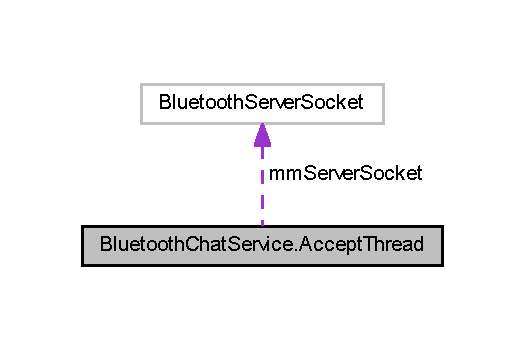
\includegraphics[width=252pt]{classcom_1_1example_1_1android_1_1_bluetooth_chat_1_1_bluetooth_chat_service_1_1_accept_thread__coll__graph}
\end{center}
\end{figure}
\subsection*{Public Member Functions}
\begin{DoxyCompactItemize}
\item 
\hyperlink{classcom_1_1example_1_1android_1_1_bluetooth_chat_1_1_bluetooth_chat_service_1_1_accept_thread_a87e04948833d0fd4826daa3f527b2153}{Accept\-Thread} ()
\item 
void \hyperlink{classcom_1_1example_1_1android_1_1_bluetooth_chat_1_1_bluetooth_chat_service_1_1_accept_thread_a13a43e6d814de94978c515cb084873b1}{run} ()
\item 
void \hyperlink{classcom_1_1example_1_1android_1_1_bluetooth_chat_1_1_bluetooth_chat_service_1_1_accept_thread_a02d5fa6b14e221f3012a794b905be166}{cancel} ()
\end{DoxyCompactItemize}
\subsection*{Private Attributes}
\begin{DoxyCompactItemize}
\item 
final Bluetooth\-Server\-Socket \hyperlink{classcom_1_1example_1_1android_1_1_bluetooth_chat_1_1_bluetooth_chat_service_1_1_accept_thread_a0b04e3279c0cd8ff1bc19ab19c7539d9}{mm\-Server\-Socket}
\end{DoxyCompactItemize}


\subsection{Detailed Description}
This thread runs while listening for incoming connections. It behaves like a server-\/side client. It runs until a connection is accepted (or until cancelled). 

\subsection{Constructor \& Destructor Documentation}
\hypertarget{classcom_1_1example_1_1android_1_1_bluetooth_chat_1_1_bluetooth_chat_service_1_1_accept_thread_a87e04948833d0fd4826daa3f527b2153}{\index{com\-::example\-::android\-::\-Bluetooth\-Chat\-::\-Bluetooth\-Chat\-Service\-::\-Accept\-Thread@{com\-::example\-::android\-::\-Bluetooth\-Chat\-::\-Bluetooth\-Chat\-Service\-::\-Accept\-Thread}!Accept\-Thread@{Accept\-Thread}}
\index{Accept\-Thread@{Accept\-Thread}!com::example::android::BluetoothChat::BluetoothChatService::AcceptThread@{com\-::example\-::android\-::\-Bluetooth\-Chat\-::\-Bluetooth\-Chat\-Service\-::\-Accept\-Thread}}
\subsubsection[{Accept\-Thread}]{\setlength{\rightskip}{0pt plus 5cm}{\bf Accept\-Thread} (
\begin{DoxyParamCaption}
{}
\end{DoxyParamCaption}
)\hspace{0.3cm}{\ttfamily  \mbox{[}inline\mbox{]}}}}\label{classcom_1_1example_1_1android_1_1_bluetooth_chat_1_1_bluetooth_chat_service_1_1_accept_thread_a87e04948833d0fd4826daa3f527b2153}


\subsection{Member Function Documentation}
\hypertarget{classcom_1_1example_1_1android_1_1_bluetooth_chat_1_1_bluetooth_chat_service_1_1_accept_thread_a02d5fa6b14e221f3012a794b905be166}{\index{com\-::example\-::android\-::\-Bluetooth\-Chat\-::\-Bluetooth\-Chat\-Service\-::\-Accept\-Thread@{com\-::example\-::android\-::\-Bluetooth\-Chat\-::\-Bluetooth\-Chat\-Service\-::\-Accept\-Thread}!cancel@{cancel}}
\index{cancel@{cancel}!com::example::android::BluetoothChat::BluetoothChatService::AcceptThread@{com\-::example\-::android\-::\-Bluetooth\-Chat\-::\-Bluetooth\-Chat\-Service\-::\-Accept\-Thread}}
\subsubsection[{cancel}]{\setlength{\rightskip}{0pt plus 5cm}void {\bf cancel} (
\begin{DoxyParamCaption}
{}
\end{DoxyParamCaption}
)\hspace{0.3cm}{\ttfamily  \mbox{[}inline\mbox{]}}}}\label{classcom_1_1example_1_1android_1_1_bluetooth_chat_1_1_bluetooth_chat_service_1_1_accept_thread_a02d5fa6b14e221f3012a794b905be166}


Here is the caller graph for this function\-:\nopagebreak
\begin{figure}[H]
\begin{center}
\leavevmode
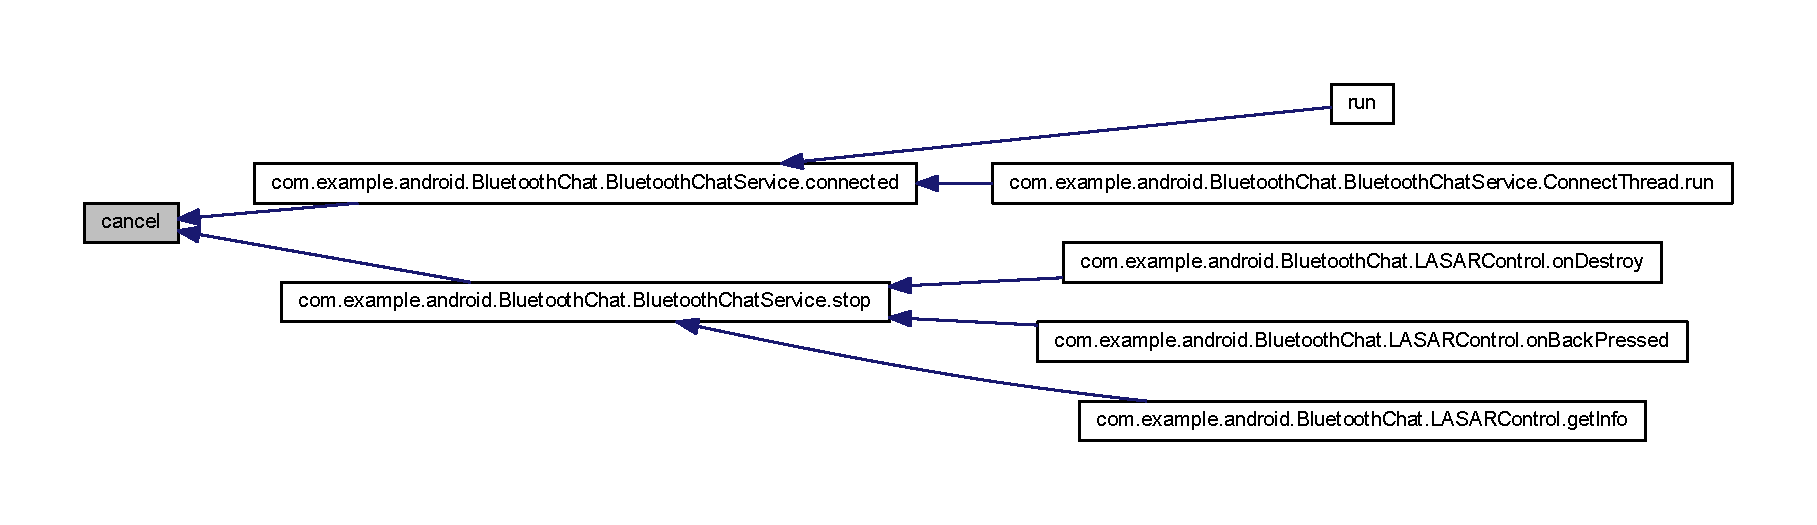
\includegraphics[width=350pt]{classcom_1_1example_1_1android_1_1_bluetooth_chat_1_1_bluetooth_chat_service_1_1_accept_thread_a02d5fa6b14e221f3012a794b905be166_icgraph}
\end{center}
\end{figure}


\hypertarget{classcom_1_1example_1_1android_1_1_bluetooth_chat_1_1_bluetooth_chat_service_1_1_accept_thread_a13a43e6d814de94978c515cb084873b1}{\index{com\-::example\-::android\-::\-Bluetooth\-Chat\-::\-Bluetooth\-Chat\-Service\-::\-Accept\-Thread@{com\-::example\-::android\-::\-Bluetooth\-Chat\-::\-Bluetooth\-Chat\-Service\-::\-Accept\-Thread}!run@{run}}
\index{run@{run}!com::example::android::BluetoothChat::BluetoothChatService::AcceptThread@{com\-::example\-::android\-::\-Bluetooth\-Chat\-::\-Bluetooth\-Chat\-Service\-::\-Accept\-Thread}}
\subsubsection[{run}]{\setlength{\rightskip}{0pt plus 5cm}void {\bf run} (
\begin{DoxyParamCaption}
{}
\end{DoxyParamCaption}
)\hspace{0.3cm}{\ttfamily  \mbox{[}inline\mbox{]}}}}\label{classcom_1_1example_1_1android_1_1_bluetooth_chat_1_1_bluetooth_chat_service_1_1_accept_thread_a13a43e6d814de94978c515cb084873b1}


Here is the call graph for this function\-:\nopagebreak
\begin{figure}[H]
\begin{center}
\leavevmode
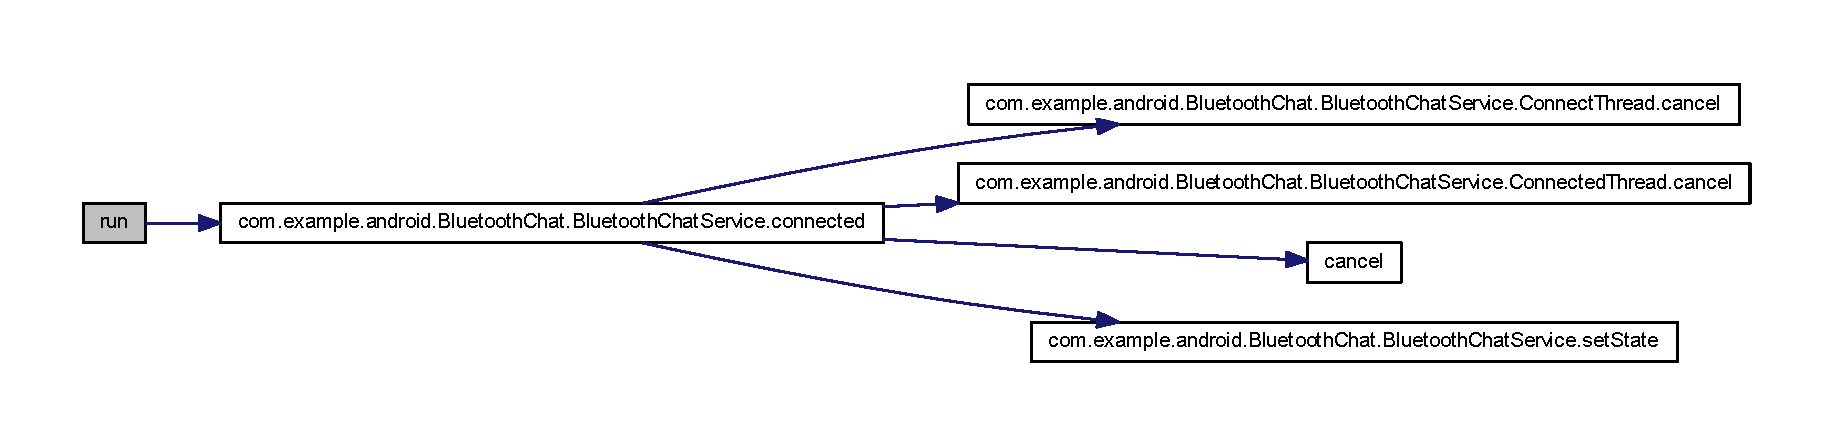
\includegraphics[width=350pt]{classcom_1_1example_1_1android_1_1_bluetooth_chat_1_1_bluetooth_chat_service_1_1_accept_thread_a13a43e6d814de94978c515cb084873b1_cgraph}
\end{center}
\end{figure}




\subsection{Field Documentation}
\hypertarget{classcom_1_1example_1_1android_1_1_bluetooth_chat_1_1_bluetooth_chat_service_1_1_accept_thread_a0b04e3279c0cd8ff1bc19ab19c7539d9}{\index{com\-::example\-::android\-::\-Bluetooth\-Chat\-::\-Bluetooth\-Chat\-Service\-::\-Accept\-Thread@{com\-::example\-::android\-::\-Bluetooth\-Chat\-::\-Bluetooth\-Chat\-Service\-::\-Accept\-Thread}!mm\-Server\-Socket@{mm\-Server\-Socket}}
\index{mm\-Server\-Socket@{mm\-Server\-Socket}!com::example::android::BluetoothChat::BluetoothChatService::AcceptThread@{com\-::example\-::android\-::\-Bluetooth\-Chat\-::\-Bluetooth\-Chat\-Service\-::\-Accept\-Thread}}
\subsubsection[{mm\-Server\-Socket}]{\setlength{\rightskip}{0pt plus 5cm}final Bluetooth\-Server\-Socket {\bf mm\-Server\-Socket}\hspace{0.3cm}{\ttfamily  \mbox{[}private\mbox{]}}}}\label{classcom_1_1example_1_1android_1_1_bluetooth_chat_1_1_bluetooth_chat_service_1_1_accept_thread_a0b04e3279c0cd8ff1bc19ab19c7539d9}


The documentation for this class was generated from the following file\-:\begin{DoxyCompactItemize}
\item 
Code/\-L\-A\-S\-A\-R/\-Android/\-L\-A\-S\-A\-R Control/src/com/example/android/\-Bluetooth\-Chat/\hyperlink{_bluetooth_chat_service_8java}{Bluetooth\-Chat\-Service.\-java}\end{DoxyCompactItemize}

\hypertarget{classcom_1_1example_1_1android_1_1_bluetooth_chat_1_1_bluetooth_chat_service}{\section{Bluetooth\-Chat\-Service Class Reference}
\label{classcom_1_1example_1_1android_1_1_bluetooth_chat_1_1_bluetooth_chat_service}\index{Bluetooth\-Chat\-Service@{Bluetooth\-Chat\-Service}}
}


Collaboration diagram for Bluetooth\-Chat\-Service\-:\nopagebreak
\begin{figure}[H]
\begin{center}
\leavevmode
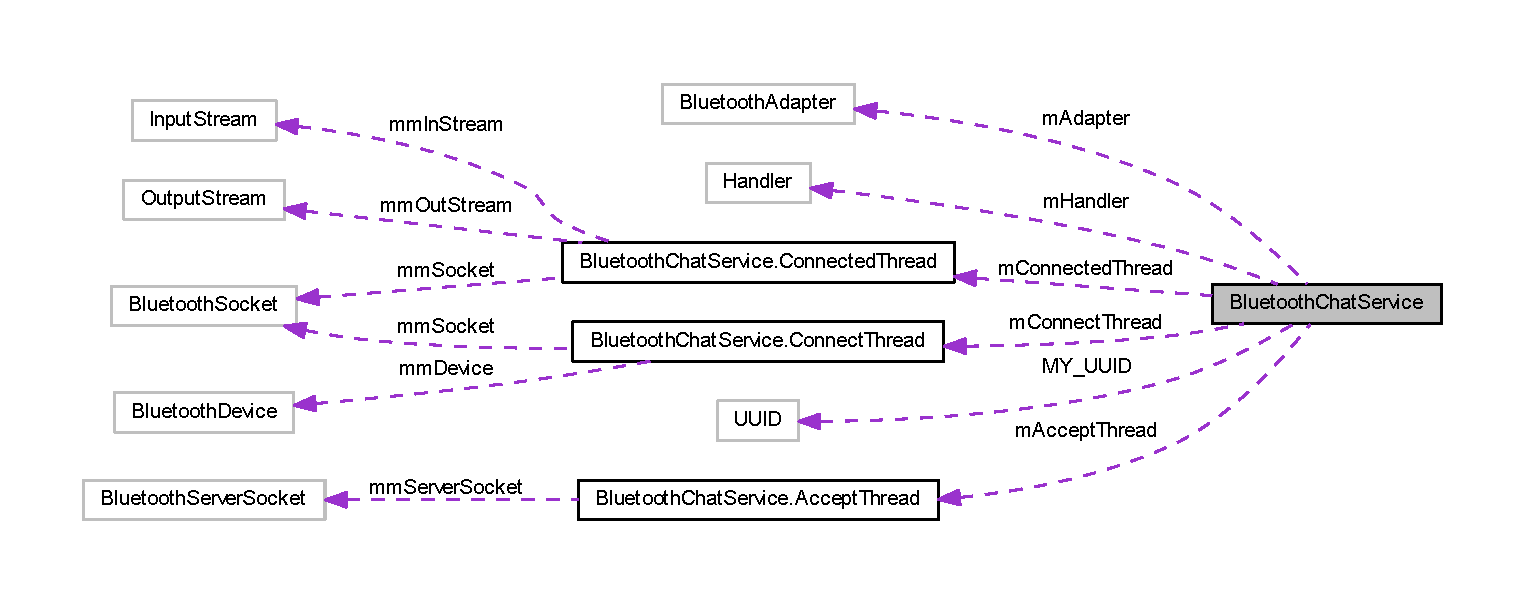
\includegraphics[width=350pt]{classcom_1_1example_1_1android_1_1_bluetooth_chat_1_1_bluetooth_chat_service__coll__graph}
\end{center}
\end{figure}
\subsection*{Data Structures}
\begin{DoxyCompactItemize}
\item 
class \hyperlink{classcom_1_1example_1_1android_1_1_bluetooth_chat_1_1_bluetooth_chat_service_1_1_accept_thread}{Accept\-Thread}
\item 
class \hyperlink{classcom_1_1example_1_1android_1_1_bluetooth_chat_1_1_bluetooth_chat_service_1_1_connected_thread}{Connected\-Thread}
\item 
class \hyperlink{classcom_1_1example_1_1android_1_1_bluetooth_chat_1_1_bluetooth_chat_service_1_1_connect_thread}{Connect\-Thread}
\end{DoxyCompactItemize}
\subsection*{Public Member Functions}
\begin{DoxyCompactItemize}
\item 
\hyperlink{classcom_1_1example_1_1android_1_1_bluetooth_chat_1_1_bluetooth_chat_service_a82aeace1fb85fa6450790cb18d9154e8}{Bluetooth\-Chat\-Service} (Context context, Handler handler)
\item 
synchronized int \hyperlink{classcom_1_1example_1_1android_1_1_bluetooth_chat_1_1_bluetooth_chat_service_a6a50c2d9aca011bf98c1ef858548b905}{get\-State} ()
\item 
synchronized void \hyperlink{classcom_1_1example_1_1android_1_1_bluetooth_chat_1_1_bluetooth_chat_service_ae3e5313b36e6f003857174584df1753e}{start} ()
\item 
synchronized void \hyperlink{classcom_1_1example_1_1android_1_1_bluetooth_chat_1_1_bluetooth_chat_service_a210e75ad8ad1a78004ee6fe643acd0aa}{connect} (Bluetooth\-Device device)
\item 
synchronized void \hyperlink{classcom_1_1example_1_1android_1_1_bluetooth_chat_1_1_bluetooth_chat_service_a7684309f45e8b4bbbe3478b7c6b7d786}{connected} (Bluetooth\-Socket socket, Bluetooth\-Device device)
\item 
synchronized void \hyperlink{classcom_1_1example_1_1android_1_1_bluetooth_chat_1_1_bluetooth_chat_service_a4bcef6dec76484d625984ace718f36fd}{stop} ()
\item 
void \hyperlink{classcom_1_1example_1_1android_1_1_bluetooth_chat_1_1_bluetooth_chat_service_a8f39f71b4e3de075a0b64236eb5ec876}{write} (byte\mbox{[}$\,$\mbox{]} out)
\end{DoxyCompactItemize}
\subsection*{Static Public Attributes}
\begin{DoxyCompactItemize}
\item 
static final int \hyperlink{classcom_1_1example_1_1android_1_1_bluetooth_chat_1_1_bluetooth_chat_service_acca6c8882253f023c0c4a78c76e07a5d}{S\-T\-A\-T\-E\-\_\-\-N\-O\-N\-E} = 0
\item 
static final int \hyperlink{classcom_1_1example_1_1android_1_1_bluetooth_chat_1_1_bluetooth_chat_service_a5b119ac8b511b1ccc522ad84810097fd}{S\-T\-A\-T\-E\-\_\-\-L\-I\-S\-T\-E\-N} = 1
\item 
static final int \hyperlink{classcom_1_1example_1_1android_1_1_bluetooth_chat_1_1_bluetooth_chat_service_a3f330f5177bb8c94ae6c8796c4839e0c}{S\-T\-A\-T\-E\-\_\-\-C\-O\-N\-N\-E\-C\-T\-I\-N\-G} = 2
\item 
static final int \hyperlink{classcom_1_1example_1_1android_1_1_bluetooth_chat_1_1_bluetooth_chat_service_a65bee812daa1c06904d2bfc9b6c98607}{S\-T\-A\-T\-E\-\_\-\-C\-O\-N\-N\-E\-C\-T\-E\-D} = 3
\end{DoxyCompactItemize}
\subsection*{Private Member Functions}
\begin{DoxyCompactItemize}
\item 
synchronized void \hyperlink{classcom_1_1example_1_1android_1_1_bluetooth_chat_1_1_bluetooth_chat_service_a09b77b92fc6c880860a3dbf4ab21e36c}{set\-State} (int state)
\item 
void \hyperlink{classcom_1_1example_1_1android_1_1_bluetooth_chat_1_1_bluetooth_chat_service_a784e1d9992765b96eb29e9ba63ad8902}{connection\-Failed} ()
\item 
void \hyperlink{classcom_1_1example_1_1android_1_1_bluetooth_chat_1_1_bluetooth_chat_service_abd4a195467743d2b3642bde9c5d2e0f6}{connection\-Lost} ()
\end{DoxyCompactItemize}
\subsection*{Private Attributes}
\begin{DoxyCompactItemize}
\item 
final Bluetooth\-Adapter \hyperlink{classcom_1_1example_1_1android_1_1_bluetooth_chat_1_1_bluetooth_chat_service_ad0137191bfc9f5f84d692c5179046dac}{m\-Adapter}
\item 
final Handler \hyperlink{classcom_1_1example_1_1android_1_1_bluetooth_chat_1_1_bluetooth_chat_service_ac596631c3faeaba71c591b7d6232c489}{m\-Handler}
\item 
\hyperlink{classcom_1_1example_1_1android_1_1_bluetooth_chat_1_1_bluetooth_chat_service_1_1_accept_thread}{Accept\-Thread} \hyperlink{classcom_1_1example_1_1android_1_1_bluetooth_chat_1_1_bluetooth_chat_service_a5e8a8695cae6c6a842646ec72feb30d7}{m\-Accept\-Thread}
\item 
\hyperlink{classcom_1_1example_1_1android_1_1_bluetooth_chat_1_1_bluetooth_chat_service_1_1_connect_thread}{Connect\-Thread} \hyperlink{classcom_1_1example_1_1android_1_1_bluetooth_chat_1_1_bluetooth_chat_service_a329b61002394a1b98ae8366549c3f4e8}{m\-Connect\-Thread}
\item 
\hyperlink{classcom_1_1example_1_1android_1_1_bluetooth_chat_1_1_bluetooth_chat_service_1_1_connected_thread}{Connected\-Thread} \hyperlink{classcom_1_1example_1_1android_1_1_bluetooth_chat_1_1_bluetooth_chat_service_a35e6f3f781880c30d3fffef2e408d367}{m\-Connected\-Thread}
\item 
int \hyperlink{classcom_1_1example_1_1android_1_1_bluetooth_chat_1_1_bluetooth_chat_service_a9170ea7c3cb727e1c86da45a7ed88a54}{m\-State}
\end{DoxyCompactItemize}
\subsection*{Static Private Attributes}
\begin{DoxyCompactItemize}
\item 
static final String \hyperlink{classcom_1_1example_1_1android_1_1_bluetooth_chat_1_1_bluetooth_chat_service_a844c5efdea72aa6bf76fb98b1072572a}{T\-A\-G} = \char`\"{}Bluetooth\-Chat\-Service\char`\"{}
\item 
static final boolean \hyperlink{classcom_1_1example_1_1android_1_1_bluetooth_chat_1_1_bluetooth_chat_service_a5d04bb9010fad999fbcad7c652d6c0ce}{D} = true
\item 
static final String \hyperlink{classcom_1_1example_1_1android_1_1_bluetooth_chat_1_1_bluetooth_chat_service_a2e2a8b5e4b33363e36e2d75ff425c86c}{N\-A\-M\-E} = \char`\"{}Bluetooth\-Chat\char`\"{}
\item 
static final U\-U\-I\-D \hyperlink{classcom_1_1example_1_1android_1_1_bluetooth_chat_1_1_bluetooth_chat_service_ad6683c9b25da0fe7ea60ab048c7589cb}{M\-Y\-\_\-\-U\-U\-I\-D} = U\-U\-I\-D.\-from\-String(\char`\"{}00001101-\/0000-\/1000-\/8000-\/00805\-F9\-B34\-F\-B\char`\"{})
\end{DoxyCompactItemize}


\subsection{Detailed Description}
This class does all the work for setting up and managing Bluetooth connections with other devices. It has a thread that listens for incoming connections, a thread for connecting with a device, and a thread for performing data transmissions when connected. 

\subsection{Constructor \& Destructor Documentation}
\hypertarget{classcom_1_1example_1_1android_1_1_bluetooth_chat_1_1_bluetooth_chat_service_a82aeace1fb85fa6450790cb18d9154e8}{\index{com\-::example\-::android\-::\-Bluetooth\-Chat\-::\-Bluetooth\-Chat\-Service@{com\-::example\-::android\-::\-Bluetooth\-Chat\-::\-Bluetooth\-Chat\-Service}!Bluetooth\-Chat\-Service@{Bluetooth\-Chat\-Service}}
\index{Bluetooth\-Chat\-Service@{Bluetooth\-Chat\-Service}!com::example::android::BluetoothChat::BluetoothChatService@{com\-::example\-::android\-::\-Bluetooth\-Chat\-::\-Bluetooth\-Chat\-Service}}
\subsubsection[{Bluetooth\-Chat\-Service}]{\setlength{\rightskip}{0pt plus 5cm}{\bf Bluetooth\-Chat\-Service} (
\begin{DoxyParamCaption}
\item[{Context}]{context, }
\item[{Handler}]{handler}
\end{DoxyParamCaption}
)\hspace{0.3cm}{\ttfamily  \mbox{[}inline\mbox{]}}}}\label{classcom_1_1example_1_1android_1_1_bluetooth_chat_1_1_bluetooth_chat_service_a82aeace1fb85fa6450790cb18d9154e8}
Constructor. Prepares a new \hyperlink{namespacecom_1_1example_1_1android_1_1_bluetooth_chat}{Bluetooth\-Chat} session. 
\begin{DoxyParams}{Parameters}
{\em context} & The U\-I Activity Context \\
\hline
{\em handler} & A Handler to send messages back to the U\-I Activity \\
\hline
\end{DoxyParams}


\subsection{Member Function Documentation}
\hypertarget{classcom_1_1example_1_1android_1_1_bluetooth_chat_1_1_bluetooth_chat_service_a210e75ad8ad1a78004ee6fe643acd0aa}{\index{com\-::example\-::android\-::\-Bluetooth\-Chat\-::\-Bluetooth\-Chat\-Service@{com\-::example\-::android\-::\-Bluetooth\-Chat\-::\-Bluetooth\-Chat\-Service}!connect@{connect}}
\index{connect@{connect}!com::example::android::BluetoothChat::BluetoothChatService@{com\-::example\-::android\-::\-Bluetooth\-Chat\-::\-Bluetooth\-Chat\-Service}}
\subsubsection[{connect}]{\setlength{\rightskip}{0pt plus 5cm}synchronized void {\bf connect} (
\begin{DoxyParamCaption}
\item[{Bluetooth\-Device}]{device}
\end{DoxyParamCaption}
)\hspace{0.3cm}{\ttfamily  \mbox{[}inline\mbox{]}}}}\label{classcom_1_1example_1_1android_1_1_bluetooth_chat_1_1_bluetooth_chat_service_a210e75ad8ad1a78004ee6fe643acd0aa}
Start the \hyperlink{classcom_1_1example_1_1android_1_1_bluetooth_chat_1_1_bluetooth_chat_service_1_1_connect_thread}{Connect\-Thread} to initiate a connection to a remote device. 
\begin{DoxyParams}{Parameters}
{\em device} & The Bluetooth\-Device to connect \\
\hline
\end{DoxyParams}


Here is the call graph for this function\-:\nopagebreak
\begin{figure}[H]
\begin{center}
\leavevmode
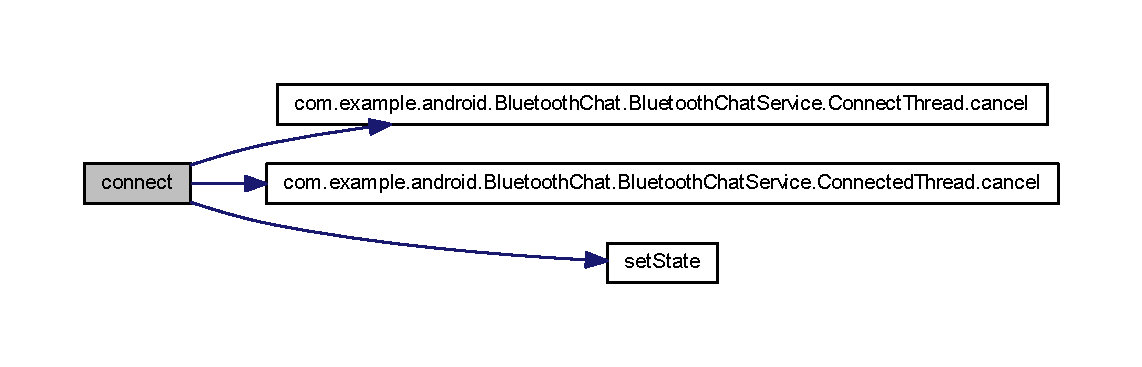
\includegraphics[width=350pt]{classcom_1_1example_1_1android_1_1_bluetooth_chat_1_1_bluetooth_chat_service_a210e75ad8ad1a78004ee6fe643acd0aa_cgraph}
\end{center}
\end{figure}




Here is the caller graph for this function\-:\nopagebreak
\begin{figure}[H]
\begin{center}
\leavevmode
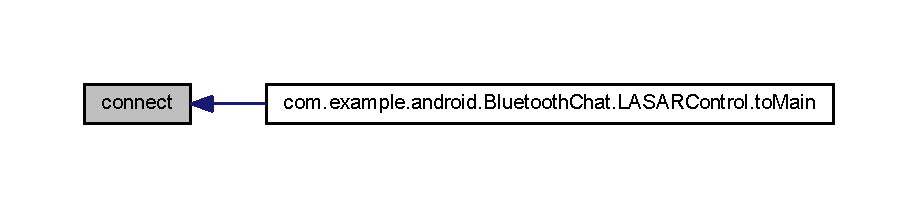
\includegraphics[width=350pt]{classcom_1_1example_1_1android_1_1_bluetooth_chat_1_1_bluetooth_chat_service_a210e75ad8ad1a78004ee6fe643acd0aa_icgraph}
\end{center}
\end{figure}


\hypertarget{classcom_1_1example_1_1android_1_1_bluetooth_chat_1_1_bluetooth_chat_service_a7684309f45e8b4bbbe3478b7c6b7d786}{\index{com\-::example\-::android\-::\-Bluetooth\-Chat\-::\-Bluetooth\-Chat\-Service@{com\-::example\-::android\-::\-Bluetooth\-Chat\-::\-Bluetooth\-Chat\-Service}!connected@{connected}}
\index{connected@{connected}!com::example::android::BluetoothChat::BluetoothChatService@{com\-::example\-::android\-::\-Bluetooth\-Chat\-::\-Bluetooth\-Chat\-Service}}
\subsubsection[{connected}]{\setlength{\rightskip}{0pt plus 5cm}synchronized void {\bf connected} (
\begin{DoxyParamCaption}
\item[{Bluetooth\-Socket}]{socket, }
\item[{Bluetooth\-Device}]{device}
\end{DoxyParamCaption}
)\hspace{0.3cm}{\ttfamily  \mbox{[}inline\mbox{]}}}}\label{classcom_1_1example_1_1android_1_1_bluetooth_chat_1_1_bluetooth_chat_service_a7684309f45e8b4bbbe3478b7c6b7d786}
Start the \hyperlink{classcom_1_1example_1_1android_1_1_bluetooth_chat_1_1_bluetooth_chat_service_1_1_connected_thread}{Connected\-Thread} to begin managing a Bluetooth connection 
\begin{DoxyParams}{Parameters}
{\em socket} & The Bluetooth\-Socket on which the connection was made \\
\hline
{\em device} & The Bluetooth\-Device that has been connected \\
\hline
\end{DoxyParams}


Here is the call graph for this function\-:
\nopagebreak
\begin{figure}[H]
\begin{center}
\leavevmode
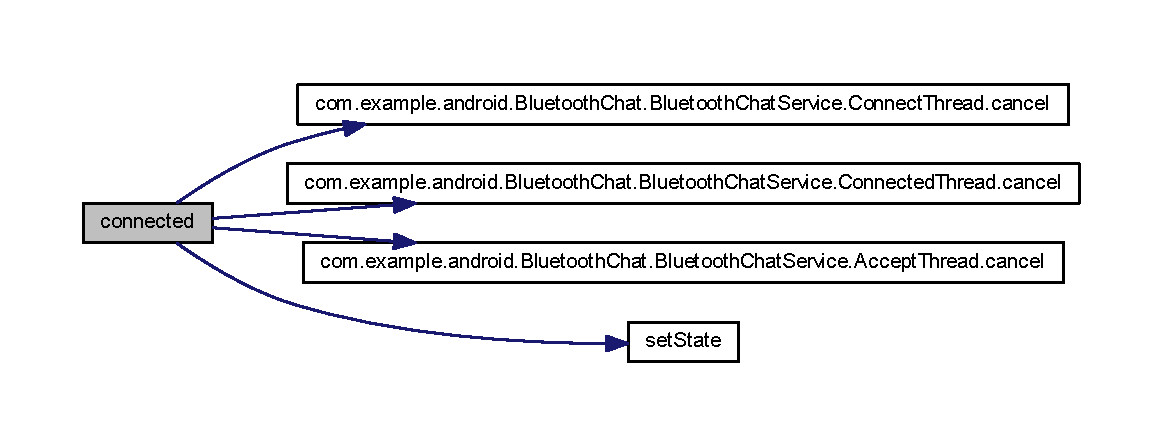
\includegraphics[width=350pt]{classcom_1_1example_1_1android_1_1_bluetooth_chat_1_1_bluetooth_chat_service_a7684309f45e8b4bbbe3478b7c6b7d786_cgraph}
\end{center}
\end{figure}




Here is the caller graph for this function\-:
\nopagebreak
\begin{figure}[H]
\begin{center}
\leavevmode
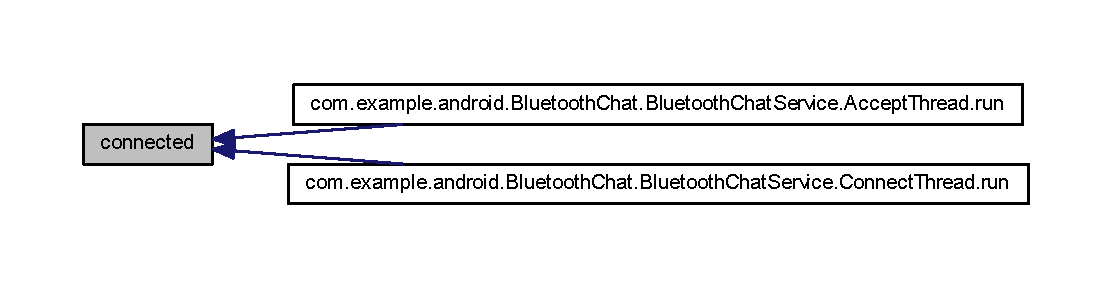
\includegraphics[width=350pt]{classcom_1_1example_1_1android_1_1_bluetooth_chat_1_1_bluetooth_chat_service_a7684309f45e8b4bbbe3478b7c6b7d786_icgraph}
\end{center}
\end{figure}


\hypertarget{classcom_1_1example_1_1android_1_1_bluetooth_chat_1_1_bluetooth_chat_service_a784e1d9992765b96eb29e9ba63ad8902}{\index{com\-::example\-::android\-::\-Bluetooth\-Chat\-::\-Bluetooth\-Chat\-Service@{com\-::example\-::android\-::\-Bluetooth\-Chat\-::\-Bluetooth\-Chat\-Service}!connection\-Failed@{connection\-Failed}}
\index{connection\-Failed@{connection\-Failed}!com::example::android::BluetoothChat::BluetoothChatService@{com\-::example\-::android\-::\-Bluetooth\-Chat\-::\-Bluetooth\-Chat\-Service}}
\subsubsection[{connection\-Failed}]{\setlength{\rightskip}{0pt plus 5cm}void {\bf connection\-Failed} (
\begin{DoxyParamCaption}
{}
\end{DoxyParamCaption}
)\hspace{0.3cm}{\ttfamily  \mbox{[}inline, private\mbox{]}}}}\label{classcom_1_1example_1_1android_1_1_bluetooth_chat_1_1_bluetooth_chat_service_a784e1d9992765b96eb29e9ba63ad8902}
Indicate that the connection attempt failed and notify the U\-I Activity. 

Here is the call graph for this function\-:
\nopagebreak
\begin{figure}[H]
\begin{center}
\leavevmode
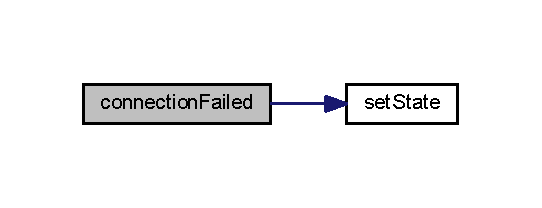
\includegraphics[width=260pt]{classcom_1_1example_1_1android_1_1_bluetooth_chat_1_1_bluetooth_chat_service_a784e1d9992765b96eb29e9ba63ad8902_cgraph}
\end{center}
\end{figure}




Here is the caller graph for this function\-:
\nopagebreak
\begin{figure}[H]
\begin{center}
\leavevmode
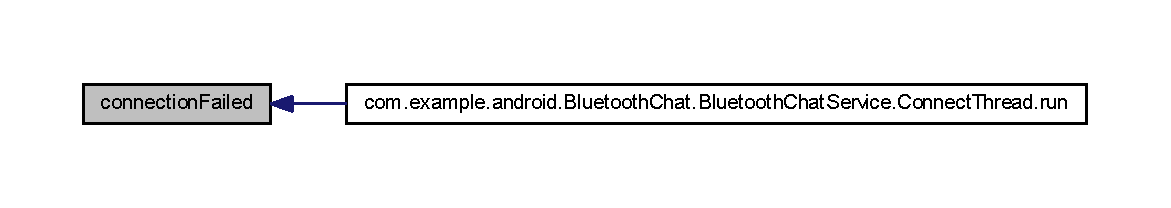
\includegraphics[width=350pt]{classcom_1_1example_1_1android_1_1_bluetooth_chat_1_1_bluetooth_chat_service_a784e1d9992765b96eb29e9ba63ad8902_icgraph}
\end{center}
\end{figure}


\hypertarget{classcom_1_1example_1_1android_1_1_bluetooth_chat_1_1_bluetooth_chat_service_abd4a195467743d2b3642bde9c5d2e0f6}{\index{com\-::example\-::android\-::\-Bluetooth\-Chat\-::\-Bluetooth\-Chat\-Service@{com\-::example\-::android\-::\-Bluetooth\-Chat\-::\-Bluetooth\-Chat\-Service}!connection\-Lost@{connection\-Lost}}
\index{connection\-Lost@{connection\-Lost}!com::example::android::BluetoothChat::BluetoothChatService@{com\-::example\-::android\-::\-Bluetooth\-Chat\-::\-Bluetooth\-Chat\-Service}}
\subsubsection[{connection\-Lost}]{\setlength{\rightskip}{0pt plus 5cm}void {\bf connection\-Lost} (
\begin{DoxyParamCaption}
{}
\end{DoxyParamCaption}
)\hspace{0.3cm}{\ttfamily  \mbox{[}inline, private\mbox{]}}}}\label{classcom_1_1example_1_1android_1_1_bluetooth_chat_1_1_bluetooth_chat_service_abd4a195467743d2b3642bde9c5d2e0f6}
Indicate that the connection was lost and notify the U\-I Activity. 

Here is the call graph for this function\-:
\nopagebreak
\begin{figure}[H]
\begin{center}
\leavevmode
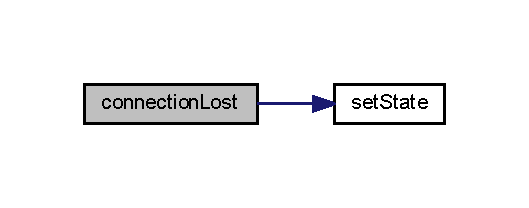
\includegraphics[width=254pt]{classcom_1_1example_1_1android_1_1_bluetooth_chat_1_1_bluetooth_chat_service_abd4a195467743d2b3642bde9c5d2e0f6_cgraph}
\end{center}
\end{figure}




Here is the caller graph for this function\-:
\nopagebreak
\begin{figure}[H]
\begin{center}
\leavevmode
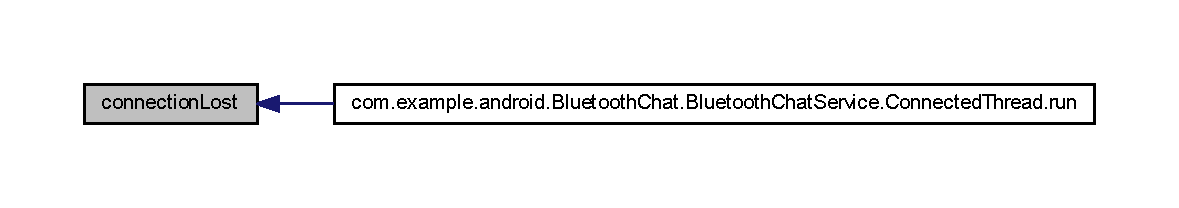
\includegraphics[width=350pt]{classcom_1_1example_1_1android_1_1_bluetooth_chat_1_1_bluetooth_chat_service_abd4a195467743d2b3642bde9c5d2e0f6_icgraph}
\end{center}
\end{figure}


\hypertarget{classcom_1_1example_1_1android_1_1_bluetooth_chat_1_1_bluetooth_chat_service_a6a50c2d9aca011bf98c1ef858548b905}{\index{com\-::example\-::android\-::\-Bluetooth\-Chat\-::\-Bluetooth\-Chat\-Service@{com\-::example\-::android\-::\-Bluetooth\-Chat\-::\-Bluetooth\-Chat\-Service}!get\-State@{get\-State}}
\index{get\-State@{get\-State}!com::example::android::BluetoothChat::BluetoothChatService@{com\-::example\-::android\-::\-Bluetooth\-Chat\-::\-Bluetooth\-Chat\-Service}}
\subsubsection[{get\-State}]{\setlength{\rightskip}{0pt plus 5cm}synchronized int {\bf get\-State} (
\begin{DoxyParamCaption}
{}
\end{DoxyParamCaption}
)\hspace{0.3cm}{\ttfamily  \mbox{[}inline\mbox{]}}}}\label{classcom_1_1example_1_1android_1_1_bluetooth_chat_1_1_bluetooth_chat_service_a6a50c2d9aca011bf98c1ef858548b905}
Return the current connection state. 

Here is the caller graph for this function\-:
\nopagebreak
\begin{figure}[H]
\begin{center}
\leavevmode
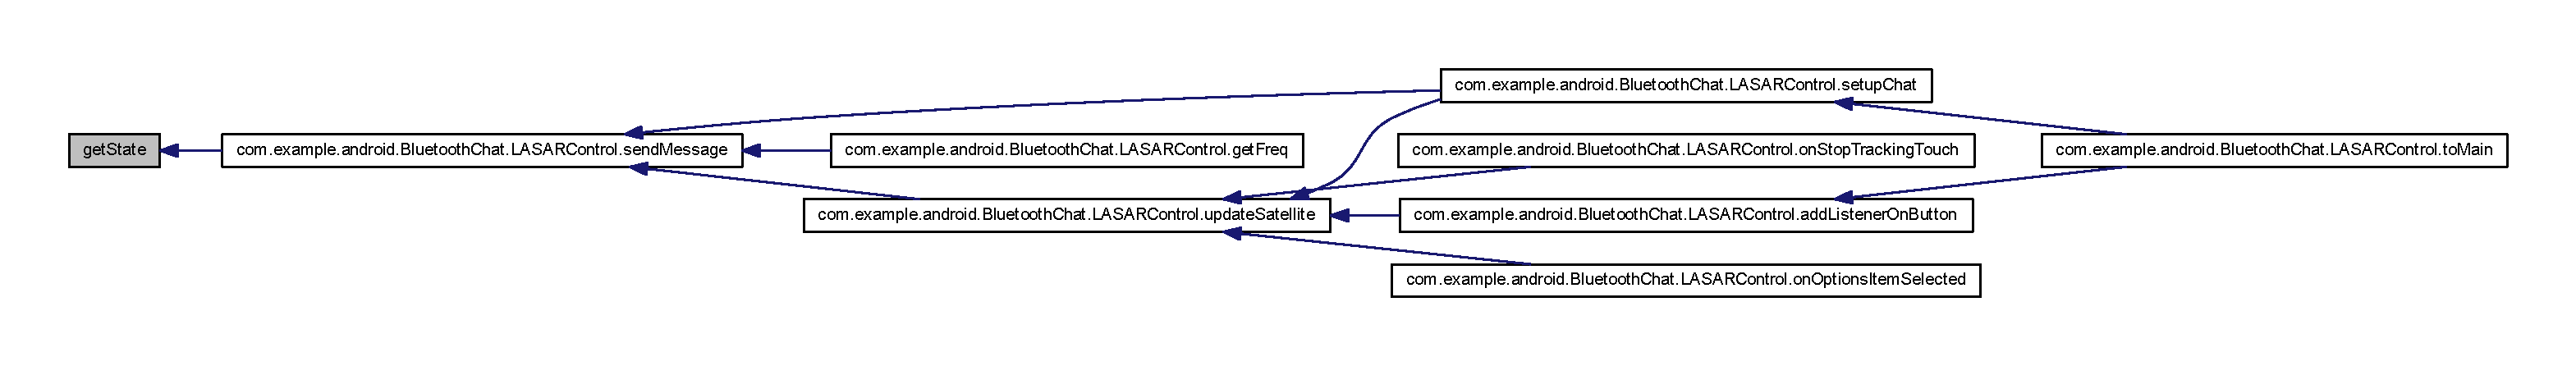
\includegraphics[width=350pt]{classcom_1_1example_1_1android_1_1_bluetooth_chat_1_1_bluetooth_chat_service_a6a50c2d9aca011bf98c1ef858548b905_icgraph}
\end{center}
\end{figure}


\hypertarget{classcom_1_1example_1_1android_1_1_bluetooth_chat_1_1_bluetooth_chat_service_a09b77b92fc6c880860a3dbf4ab21e36c}{\index{com\-::example\-::android\-::\-Bluetooth\-Chat\-::\-Bluetooth\-Chat\-Service@{com\-::example\-::android\-::\-Bluetooth\-Chat\-::\-Bluetooth\-Chat\-Service}!set\-State@{set\-State}}
\index{set\-State@{set\-State}!com::example::android::BluetoothChat::BluetoothChatService@{com\-::example\-::android\-::\-Bluetooth\-Chat\-::\-Bluetooth\-Chat\-Service}}
\subsubsection[{set\-State}]{\setlength{\rightskip}{0pt plus 5cm}synchronized void {\bf set\-State} (
\begin{DoxyParamCaption}
\item[{int}]{state}
\end{DoxyParamCaption}
)\hspace{0.3cm}{\ttfamily  \mbox{[}inline, private\mbox{]}}}}\label{classcom_1_1example_1_1android_1_1_bluetooth_chat_1_1_bluetooth_chat_service_a09b77b92fc6c880860a3dbf4ab21e36c}
Set the current state of the chat connection 
\begin{DoxyParams}{Parameters}
{\em state} & An integer defining the current connection state \\
\hline
\end{DoxyParams}


Here is the caller graph for this function\-:
\nopagebreak
\begin{figure}[H]
\begin{center}
\leavevmode
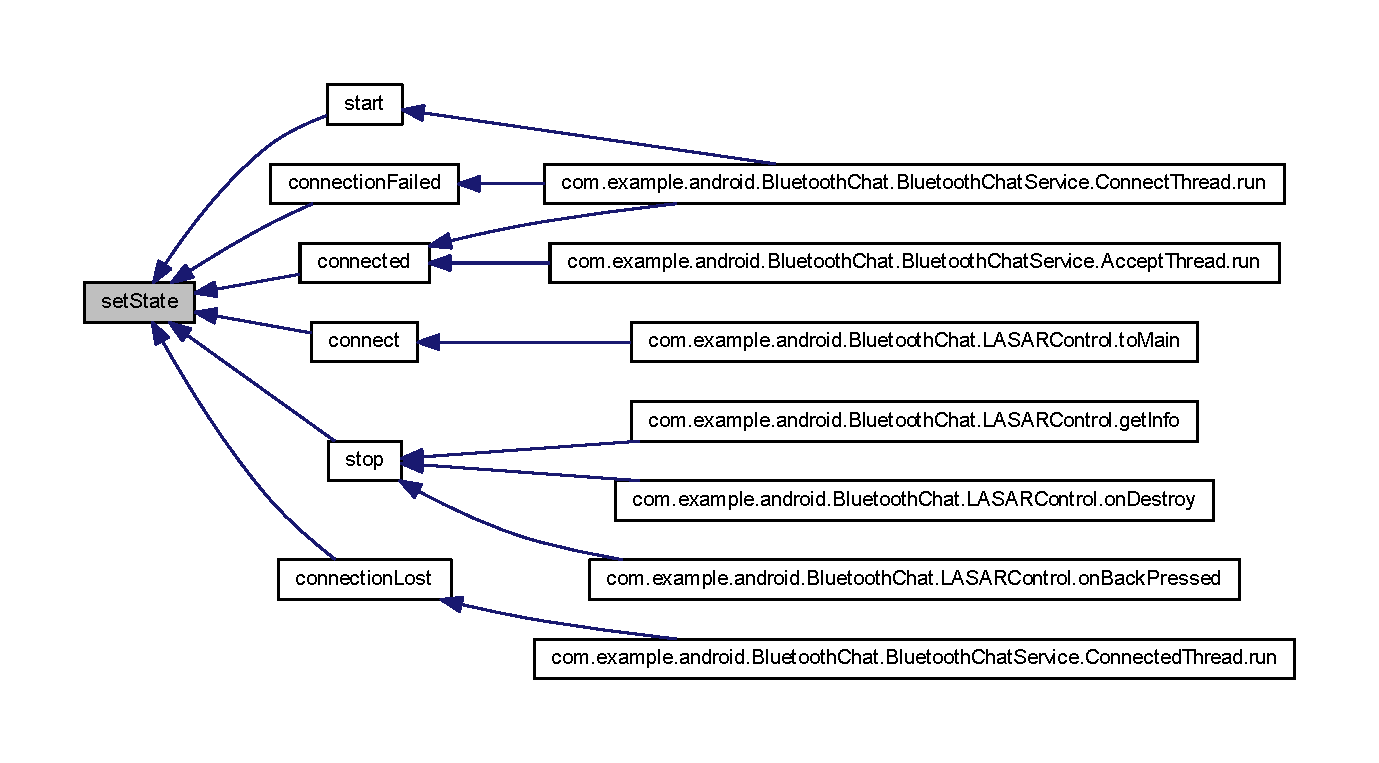
\includegraphics[width=350pt]{classcom_1_1example_1_1android_1_1_bluetooth_chat_1_1_bluetooth_chat_service_a09b77b92fc6c880860a3dbf4ab21e36c_icgraph}
\end{center}
\end{figure}


\hypertarget{classcom_1_1example_1_1android_1_1_bluetooth_chat_1_1_bluetooth_chat_service_ae3e5313b36e6f003857174584df1753e}{\index{com\-::example\-::android\-::\-Bluetooth\-Chat\-::\-Bluetooth\-Chat\-Service@{com\-::example\-::android\-::\-Bluetooth\-Chat\-::\-Bluetooth\-Chat\-Service}!start@{start}}
\index{start@{start}!com::example::android::BluetoothChat::BluetoothChatService@{com\-::example\-::android\-::\-Bluetooth\-Chat\-::\-Bluetooth\-Chat\-Service}}
\subsubsection[{start}]{\setlength{\rightskip}{0pt plus 5cm}synchronized void {\bf start} (
\begin{DoxyParamCaption}
{}
\end{DoxyParamCaption}
)\hspace{0.3cm}{\ttfamily  \mbox{[}inline\mbox{]}}}}\label{classcom_1_1example_1_1android_1_1_bluetooth_chat_1_1_bluetooth_chat_service_ae3e5313b36e6f003857174584df1753e}
Start the chat service. Specifically start \hyperlink{classcom_1_1example_1_1android_1_1_bluetooth_chat_1_1_bluetooth_chat_service_1_1_accept_thread}{Accept\-Thread} to begin a session in listening (server) mode. Called by the Activity on\-Resume() 

Here is the call graph for this function\-:
\nopagebreak
\begin{figure}[H]
\begin{center}
\leavevmode
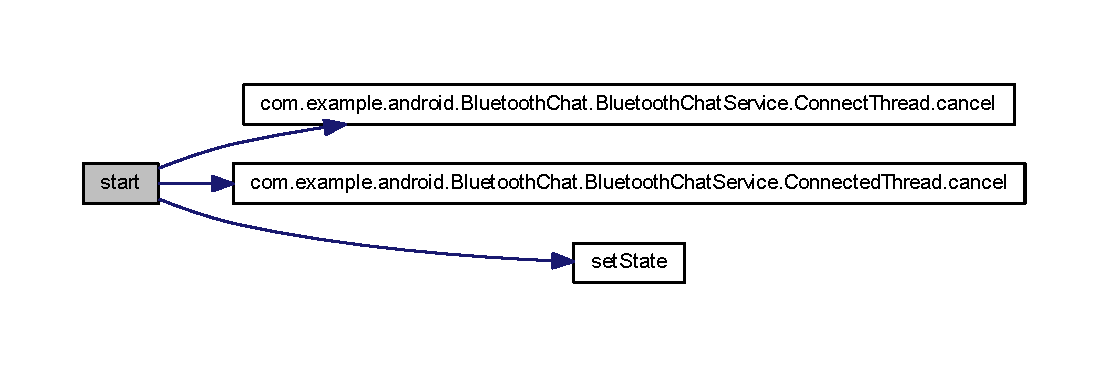
\includegraphics[width=350pt]{classcom_1_1example_1_1android_1_1_bluetooth_chat_1_1_bluetooth_chat_service_ae3e5313b36e6f003857174584df1753e_cgraph}
\end{center}
\end{figure}




Here is the caller graph for this function\-:
\nopagebreak
\begin{figure}[H]
\begin{center}
\leavevmode
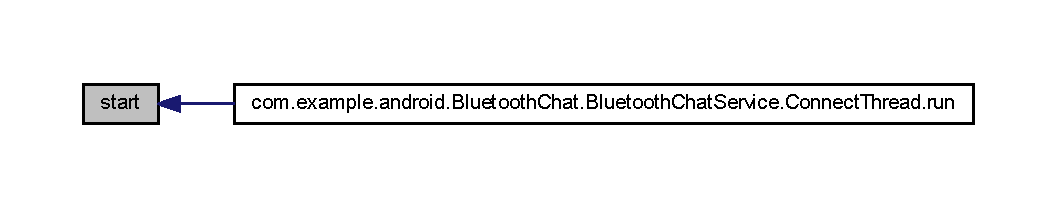
\includegraphics[width=350pt]{classcom_1_1example_1_1android_1_1_bluetooth_chat_1_1_bluetooth_chat_service_ae3e5313b36e6f003857174584df1753e_icgraph}
\end{center}
\end{figure}


\hypertarget{classcom_1_1example_1_1android_1_1_bluetooth_chat_1_1_bluetooth_chat_service_a4bcef6dec76484d625984ace718f36fd}{\index{com\-::example\-::android\-::\-Bluetooth\-Chat\-::\-Bluetooth\-Chat\-Service@{com\-::example\-::android\-::\-Bluetooth\-Chat\-::\-Bluetooth\-Chat\-Service}!stop@{stop}}
\index{stop@{stop}!com::example::android::BluetoothChat::BluetoothChatService@{com\-::example\-::android\-::\-Bluetooth\-Chat\-::\-Bluetooth\-Chat\-Service}}
\subsubsection[{stop}]{\setlength{\rightskip}{0pt plus 5cm}synchronized void {\bf stop} (
\begin{DoxyParamCaption}
{}
\end{DoxyParamCaption}
)\hspace{0.3cm}{\ttfamily  \mbox{[}inline\mbox{]}}}}\label{classcom_1_1example_1_1android_1_1_bluetooth_chat_1_1_bluetooth_chat_service_a4bcef6dec76484d625984ace718f36fd}
Stop all threads 

Here is the call graph for this function\-:
\nopagebreak
\begin{figure}[H]
\begin{center}
\leavevmode
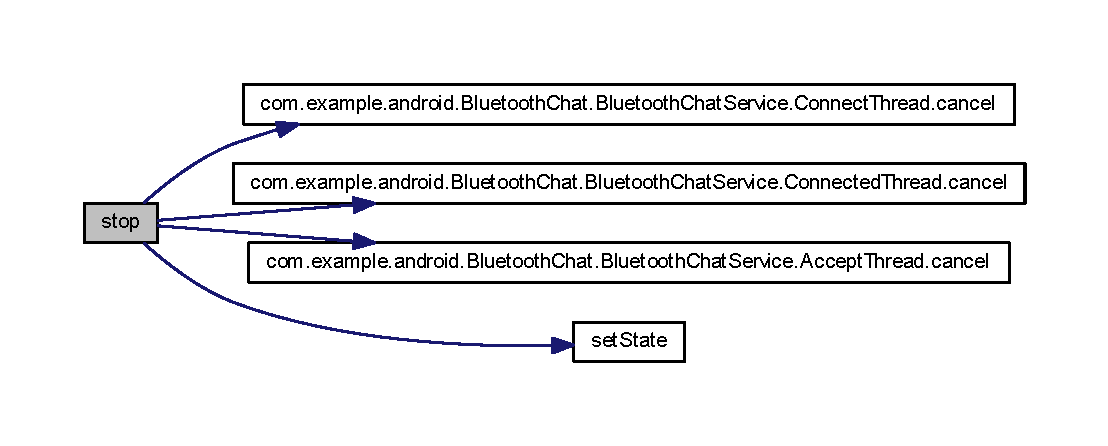
\includegraphics[width=350pt]{classcom_1_1example_1_1android_1_1_bluetooth_chat_1_1_bluetooth_chat_service_a4bcef6dec76484d625984ace718f36fd_cgraph}
\end{center}
\end{figure}




Here is the caller graph for this function\-:
\nopagebreak
\begin{figure}[H]
\begin{center}
\leavevmode
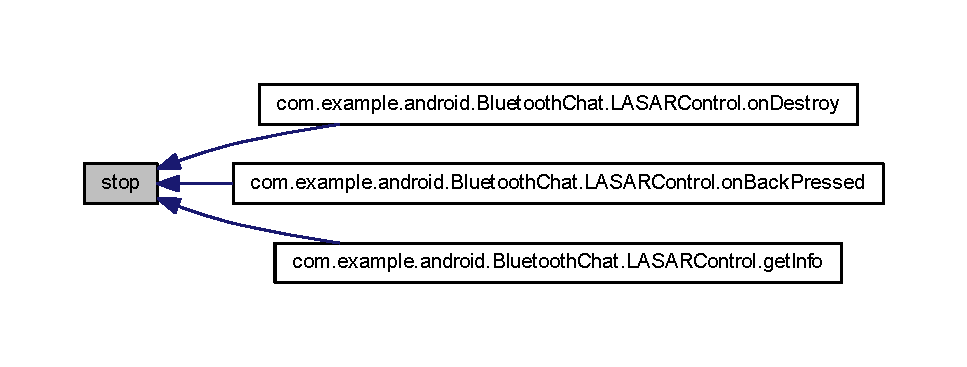
\includegraphics[width=350pt]{classcom_1_1example_1_1android_1_1_bluetooth_chat_1_1_bluetooth_chat_service_a4bcef6dec76484d625984ace718f36fd_icgraph}
\end{center}
\end{figure}


\hypertarget{classcom_1_1example_1_1android_1_1_bluetooth_chat_1_1_bluetooth_chat_service_a8f39f71b4e3de075a0b64236eb5ec876}{\index{com\-::example\-::android\-::\-Bluetooth\-Chat\-::\-Bluetooth\-Chat\-Service@{com\-::example\-::android\-::\-Bluetooth\-Chat\-::\-Bluetooth\-Chat\-Service}!write@{write}}
\index{write@{write}!com::example::android::BluetoothChat::BluetoothChatService@{com\-::example\-::android\-::\-Bluetooth\-Chat\-::\-Bluetooth\-Chat\-Service}}
\subsubsection[{write}]{\setlength{\rightskip}{0pt plus 5cm}void {\bf write} (
\begin{DoxyParamCaption}
\item[{byte\mbox{[}$\,$\mbox{]}}]{out}
\end{DoxyParamCaption}
)\hspace{0.3cm}{\ttfamily  \mbox{[}inline\mbox{]}}}}\label{classcom_1_1example_1_1android_1_1_bluetooth_chat_1_1_bluetooth_chat_service_a8f39f71b4e3de075a0b64236eb5ec876}
Write to the \hyperlink{classcom_1_1example_1_1android_1_1_bluetooth_chat_1_1_bluetooth_chat_service_1_1_connected_thread}{Connected\-Thread} in an unsynchronized manner 
\begin{DoxyParams}{Parameters}
{\em out} & The bytes to write \\
\hline
\end{DoxyParams}
\begin{DoxySeeAlso}{See also}
\hyperlink{classcom_1_1example_1_1android_1_1_bluetooth_chat_1_1_bluetooth_chat_service_1_1_connected_thread_ae29f62e52ac434bc0b80facee55ff1c8}{Connected\-Thread\-::write(byte\mbox{[}$\,$\mbox{]})} 
\end{DoxySeeAlso}


Here is the call graph for this function\-:
\nopagebreak
\begin{figure}[H]
\begin{center}
\leavevmode
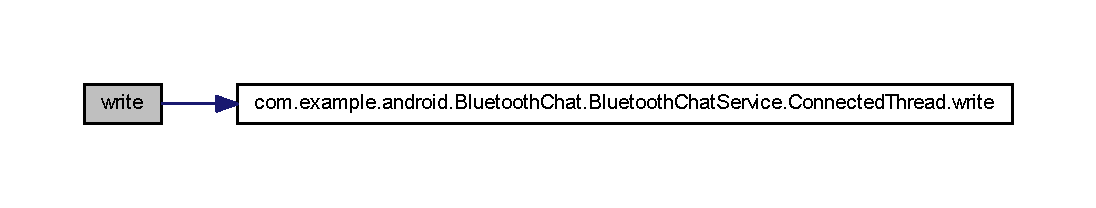
\includegraphics[width=350pt]{classcom_1_1example_1_1android_1_1_bluetooth_chat_1_1_bluetooth_chat_service_a8f39f71b4e3de075a0b64236eb5ec876_cgraph}
\end{center}
\end{figure}




Here is the caller graph for this function\-:
\nopagebreak
\begin{figure}[H]
\begin{center}
\leavevmode
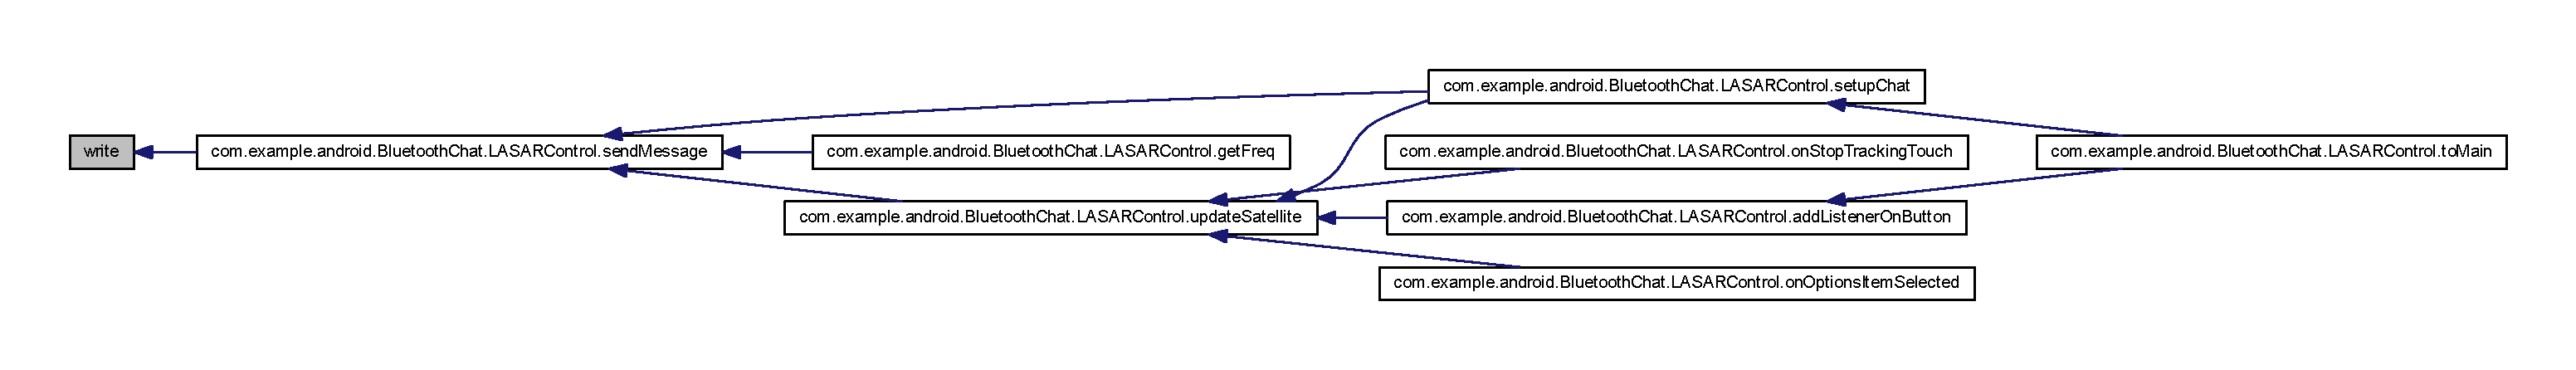
\includegraphics[width=350pt]{classcom_1_1example_1_1android_1_1_bluetooth_chat_1_1_bluetooth_chat_service_a8f39f71b4e3de075a0b64236eb5ec876_icgraph}
\end{center}
\end{figure}




\subsection{Field Documentation}
\hypertarget{classcom_1_1example_1_1android_1_1_bluetooth_chat_1_1_bluetooth_chat_service_a5d04bb9010fad999fbcad7c652d6c0ce}{\index{com\-::example\-::android\-::\-Bluetooth\-Chat\-::\-Bluetooth\-Chat\-Service@{com\-::example\-::android\-::\-Bluetooth\-Chat\-::\-Bluetooth\-Chat\-Service}!D@{D}}
\index{D@{D}!com::example::android::BluetoothChat::BluetoothChatService@{com\-::example\-::android\-::\-Bluetooth\-Chat\-::\-Bluetooth\-Chat\-Service}}
\subsubsection[{D}]{\setlength{\rightskip}{0pt plus 5cm}final boolean {\bf D} = true\hspace{0.3cm}{\ttfamily  \mbox{[}static, private\mbox{]}}}}\label{classcom_1_1example_1_1android_1_1_bluetooth_chat_1_1_bluetooth_chat_service_a5d04bb9010fad999fbcad7c652d6c0ce}
\hypertarget{classcom_1_1example_1_1android_1_1_bluetooth_chat_1_1_bluetooth_chat_service_a5e8a8695cae6c6a842646ec72feb30d7}{\index{com\-::example\-::android\-::\-Bluetooth\-Chat\-::\-Bluetooth\-Chat\-Service@{com\-::example\-::android\-::\-Bluetooth\-Chat\-::\-Bluetooth\-Chat\-Service}!m\-Accept\-Thread@{m\-Accept\-Thread}}
\index{m\-Accept\-Thread@{m\-Accept\-Thread}!com::example::android::BluetoothChat::BluetoothChatService@{com\-::example\-::android\-::\-Bluetooth\-Chat\-::\-Bluetooth\-Chat\-Service}}
\subsubsection[{m\-Accept\-Thread}]{\setlength{\rightskip}{0pt plus 5cm}{\bf Accept\-Thread} {\bf m\-Accept\-Thread}\hspace{0.3cm}{\ttfamily  \mbox{[}private\mbox{]}}}}\label{classcom_1_1example_1_1android_1_1_bluetooth_chat_1_1_bluetooth_chat_service_a5e8a8695cae6c6a842646ec72feb30d7}
\hypertarget{classcom_1_1example_1_1android_1_1_bluetooth_chat_1_1_bluetooth_chat_service_ad0137191bfc9f5f84d692c5179046dac}{\index{com\-::example\-::android\-::\-Bluetooth\-Chat\-::\-Bluetooth\-Chat\-Service@{com\-::example\-::android\-::\-Bluetooth\-Chat\-::\-Bluetooth\-Chat\-Service}!m\-Adapter@{m\-Adapter}}
\index{m\-Adapter@{m\-Adapter}!com::example::android::BluetoothChat::BluetoothChatService@{com\-::example\-::android\-::\-Bluetooth\-Chat\-::\-Bluetooth\-Chat\-Service}}
\subsubsection[{m\-Adapter}]{\setlength{\rightskip}{0pt plus 5cm}final Bluetooth\-Adapter {\bf m\-Adapter}\hspace{0.3cm}{\ttfamily  \mbox{[}private\mbox{]}}}}\label{classcom_1_1example_1_1android_1_1_bluetooth_chat_1_1_bluetooth_chat_service_ad0137191bfc9f5f84d692c5179046dac}
\hypertarget{classcom_1_1example_1_1android_1_1_bluetooth_chat_1_1_bluetooth_chat_service_a35e6f3f781880c30d3fffef2e408d367}{\index{com\-::example\-::android\-::\-Bluetooth\-Chat\-::\-Bluetooth\-Chat\-Service@{com\-::example\-::android\-::\-Bluetooth\-Chat\-::\-Bluetooth\-Chat\-Service}!m\-Connected\-Thread@{m\-Connected\-Thread}}
\index{m\-Connected\-Thread@{m\-Connected\-Thread}!com::example::android::BluetoothChat::BluetoothChatService@{com\-::example\-::android\-::\-Bluetooth\-Chat\-::\-Bluetooth\-Chat\-Service}}
\subsubsection[{m\-Connected\-Thread}]{\setlength{\rightskip}{0pt plus 5cm}{\bf Connected\-Thread} {\bf m\-Connected\-Thread}\hspace{0.3cm}{\ttfamily  \mbox{[}private\mbox{]}}}}\label{classcom_1_1example_1_1android_1_1_bluetooth_chat_1_1_bluetooth_chat_service_a35e6f3f781880c30d3fffef2e408d367}
\hypertarget{classcom_1_1example_1_1android_1_1_bluetooth_chat_1_1_bluetooth_chat_service_a329b61002394a1b98ae8366549c3f4e8}{\index{com\-::example\-::android\-::\-Bluetooth\-Chat\-::\-Bluetooth\-Chat\-Service@{com\-::example\-::android\-::\-Bluetooth\-Chat\-::\-Bluetooth\-Chat\-Service}!m\-Connect\-Thread@{m\-Connect\-Thread}}
\index{m\-Connect\-Thread@{m\-Connect\-Thread}!com::example::android::BluetoothChat::BluetoothChatService@{com\-::example\-::android\-::\-Bluetooth\-Chat\-::\-Bluetooth\-Chat\-Service}}
\subsubsection[{m\-Connect\-Thread}]{\setlength{\rightskip}{0pt plus 5cm}{\bf Connect\-Thread} {\bf m\-Connect\-Thread}\hspace{0.3cm}{\ttfamily  \mbox{[}private\mbox{]}}}}\label{classcom_1_1example_1_1android_1_1_bluetooth_chat_1_1_bluetooth_chat_service_a329b61002394a1b98ae8366549c3f4e8}
\hypertarget{classcom_1_1example_1_1android_1_1_bluetooth_chat_1_1_bluetooth_chat_service_ac596631c3faeaba71c591b7d6232c489}{\index{com\-::example\-::android\-::\-Bluetooth\-Chat\-::\-Bluetooth\-Chat\-Service@{com\-::example\-::android\-::\-Bluetooth\-Chat\-::\-Bluetooth\-Chat\-Service}!m\-Handler@{m\-Handler}}
\index{m\-Handler@{m\-Handler}!com::example::android::BluetoothChat::BluetoothChatService@{com\-::example\-::android\-::\-Bluetooth\-Chat\-::\-Bluetooth\-Chat\-Service}}
\subsubsection[{m\-Handler}]{\setlength{\rightskip}{0pt plus 5cm}final Handler {\bf m\-Handler}\hspace{0.3cm}{\ttfamily  \mbox{[}private\mbox{]}}}}\label{classcom_1_1example_1_1android_1_1_bluetooth_chat_1_1_bluetooth_chat_service_ac596631c3faeaba71c591b7d6232c489}
\hypertarget{classcom_1_1example_1_1android_1_1_bluetooth_chat_1_1_bluetooth_chat_service_a9170ea7c3cb727e1c86da45a7ed88a54}{\index{com\-::example\-::android\-::\-Bluetooth\-Chat\-::\-Bluetooth\-Chat\-Service@{com\-::example\-::android\-::\-Bluetooth\-Chat\-::\-Bluetooth\-Chat\-Service}!m\-State@{m\-State}}
\index{m\-State@{m\-State}!com::example::android::BluetoothChat::BluetoothChatService@{com\-::example\-::android\-::\-Bluetooth\-Chat\-::\-Bluetooth\-Chat\-Service}}
\subsubsection[{m\-State}]{\setlength{\rightskip}{0pt plus 5cm}int {\bf m\-State}\hspace{0.3cm}{\ttfamily  \mbox{[}private\mbox{]}}}}\label{classcom_1_1example_1_1android_1_1_bluetooth_chat_1_1_bluetooth_chat_service_a9170ea7c3cb727e1c86da45a7ed88a54}
\hypertarget{classcom_1_1example_1_1android_1_1_bluetooth_chat_1_1_bluetooth_chat_service_ad6683c9b25da0fe7ea60ab048c7589cb}{\index{com\-::example\-::android\-::\-Bluetooth\-Chat\-::\-Bluetooth\-Chat\-Service@{com\-::example\-::android\-::\-Bluetooth\-Chat\-::\-Bluetooth\-Chat\-Service}!M\-Y\-\_\-\-U\-U\-I\-D@{M\-Y\-\_\-\-U\-U\-I\-D}}
\index{M\-Y\-\_\-\-U\-U\-I\-D@{M\-Y\-\_\-\-U\-U\-I\-D}!com::example::android::BluetoothChat::BluetoothChatService@{com\-::example\-::android\-::\-Bluetooth\-Chat\-::\-Bluetooth\-Chat\-Service}}
\subsubsection[{M\-Y\-\_\-\-U\-U\-I\-D}]{\setlength{\rightskip}{0pt plus 5cm}final U\-U\-I\-D {\bf M\-Y\-\_\-\-U\-U\-I\-D} = U\-U\-I\-D.\-from\-String(\char`\"{}00001101-\/0000-\/1000-\/8000-\/00805\-F9\-B34\-F\-B\char`\"{})\hspace{0.3cm}{\ttfamily  \mbox{[}static, private\mbox{]}}}}\label{classcom_1_1example_1_1android_1_1_bluetooth_chat_1_1_bluetooth_chat_service_ad6683c9b25da0fe7ea60ab048c7589cb}
\hypertarget{classcom_1_1example_1_1android_1_1_bluetooth_chat_1_1_bluetooth_chat_service_a2e2a8b5e4b33363e36e2d75ff425c86c}{\index{com\-::example\-::android\-::\-Bluetooth\-Chat\-::\-Bluetooth\-Chat\-Service@{com\-::example\-::android\-::\-Bluetooth\-Chat\-::\-Bluetooth\-Chat\-Service}!N\-A\-M\-E@{N\-A\-M\-E}}
\index{N\-A\-M\-E@{N\-A\-M\-E}!com::example::android::BluetoothChat::BluetoothChatService@{com\-::example\-::android\-::\-Bluetooth\-Chat\-::\-Bluetooth\-Chat\-Service}}
\subsubsection[{N\-A\-M\-E}]{\setlength{\rightskip}{0pt plus 5cm}final String {\bf N\-A\-M\-E} = \char`\"{}Bluetooth\-Chat\char`\"{}\hspace{0.3cm}{\ttfamily  \mbox{[}static, private\mbox{]}}}}\label{classcom_1_1example_1_1android_1_1_bluetooth_chat_1_1_bluetooth_chat_service_a2e2a8b5e4b33363e36e2d75ff425c86c}
\hypertarget{classcom_1_1example_1_1android_1_1_bluetooth_chat_1_1_bluetooth_chat_service_a65bee812daa1c06904d2bfc9b6c98607}{\index{com\-::example\-::android\-::\-Bluetooth\-Chat\-::\-Bluetooth\-Chat\-Service@{com\-::example\-::android\-::\-Bluetooth\-Chat\-::\-Bluetooth\-Chat\-Service}!S\-T\-A\-T\-E\-\_\-\-C\-O\-N\-N\-E\-C\-T\-E\-D@{S\-T\-A\-T\-E\-\_\-\-C\-O\-N\-N\-E\-C\-T\-E\-D}}
\index{S\-T\-A\-T\-E\-\_\-\-C\-O\-N\-N\-E\-C\-T\-E\-D@{S\-T\-A\-T\-E\-\_\-\-C\-O\-N\-N\-E\-C\-T\-E\-D}!com::example::android::BluetoothChat::BluetoothChatService@{com\-::example\-::android\-::\-Bluetooth\-Chat\-::\-Bluetooth\-Chat\-Service}}
\subsubsection[{S\-T\-A\-T\-E\-\_\-\-C\-O\-N\-N\-E\-C\-T\-E\-D}]{\setlength{\rightskip}{0pt plus 5cm}final int {\bf S\-T\-A\-T\-E\-\_\-\-C\-O\-N\-N\-E\-C\-T\-E\-D} = 3\hspace{0.3cm}{\ttfamily  \mbox{[}static\mbox{]}}}}\label{classcom_1_1example_1_1android_1_1_bluetooth_chat_1_1_bluetooth_chat_service_a65bee812daa1c06904d2bfc9b6c98607}
\hypertarget{classcom_1_1example_1_1android_1_1_bluetooth_chat_1_1_bluetooth_chat_service_a3f330f5177bb8c94ae6c8796c4839e0c}{\index{com\-::example\-::android\-::\-Bluetooth\-Chat\-::\-Bluetooth\-Chat\-Service@{com\-::example\-::android\-::\-Bluetooth\-Chat\-::\-Bluetooth\-Chat\-Service}!S\-T\-A\-T\-E\-\_\-\-C\-O\-N\-N\-E\-C\-T\-I\-N\-G@{S\-T\-A\-T\-E\-\_\-\-C\-O\-N\-N\-E\-C\-T\-I\-N\-G}}
\index{S\-T\-A\-T\-E\-\_\-\-C\-O\-N\-N\-E\-C\-T\-I\-N\-G@{S\-T\-A\-T\-E\-\_\-\-C\-O\-N\-N\-E\-C\-T\-I\-N\-G}!com::example::android::BluetoothChat::BluetoothChatService@{com\-::example\-::android\-::\-Bluetooth\-Chat\-::\-Bluetooth\-Chat\-Service}}
\subsubsection[{S\-T\-A\-T\-E\-\_\-\-C\-O\-N\-N\-E\-C\-T\-I\-N\-G}]{\setlength{\rightskip}{0pt plus 5cm}final int {\bf S\-T\-A\-T\-E\-\_\-\-C\-O\-N\-N\-E\-C\-T\-I\-N\-G} = 2\hspace{0.3cm}{\ttfamily  \mbox{[}static\mbox{]}}}}\label{classcom_1_1example_1_1android_1_1_bluetooth_chat_1_1_bluetooth_chat_service_a3f330f5177bb8c94ae6c8796c4839e0c}
\hypertarget{classcom_1_1example_1_1android_1_1_bluetooth_chat_1_1_bluetooth_chat_service_a5b119ac8b511b1ccc522ad84810097fd}{\index{com\-::example\-::android\-::\-Bluetooth\-Chat\-::\-Bluetooth\-Chat\-Service@{com\-::example\-::android\-::\-Bluetooth\-Chat\-::\-Bluetooth\-Chat\-Service}!S\-T\-A\-T\-E\-\_\-\-L\-I\-S\-T\-E\-N@{S\-T\-A\-T\-E\-\_\-\-L\-I\-S\-T\-E\-N}}
\index{S\-T\-A\-T\-E\-\_\-\-L\-I\-S\-T\-E\-N@{S\-T\-A\-T\-E\-\_\-\-L\-I\-S\-T\-E\-N}!com::example::android::BluetoothChat::BluetoothChatService@{com\-::example\-::android\-::\-Bluetooth\-Chat\-::\-Bluetooth\-Chat\-Service}}
\subsubsection[{S\-T\-A\-T\-E\-\_\-\-L\-I\-S\-T\-E\-N}]{\setlength{\rightskip}{0pt plus 5cm}final int {\bf S\-T\-A\-T\-E\-\_\-\-L\-I\-S\-T\-E\-N} = 1\hspace{0.3cm}{\ttfamily  \mbox{[}static\mbox{]}}}}\label{classcom_1_1example_1_1android_1_1_bluetooth_chat_1_1_bluetooth_chat_service_a5b119ac8b511b1ccc522ad84810097fd}
\hypertarget{classcom_1_1example_1_1android_1_1_bluetooth_chat_1_1_bluetooth_chat_service_acca6c8882253f023c0c4a78c76e07a5d}{\index{com\-::example\-::android\-::\-Bluetooth\-Chat\-::\-Bluetooth\-Chat\-Service@{com\-::example\-::android\-::\-Bluetooth\-Chat\-::\-Bluetooth\-Chat\-Service}!S\-T\-A\-T\-E\-\_\-\-N\-O\-N\-E@{S\-T\-A\-T\-E\-\_\-\-N\-O\-N\-E}}
\index{S\-T\-A\-T\-E\-\_\-\-N\-O\-N\-E@{S\-T\-A\-T\-E\-\_\-\-N\-O\-N\-E}!com::example::android::BluetoothChat::BluetoothChatService@{com\-::example\-::android\-::\-Bluetooth\-Chat\-::\-Bluetooth\-Chat\-Service}}
\subsubsection[{S\-T\-A\-T\-E\-\_\-\-N\-O\-N\-E}]{\setlength{\rightskip}{0pt plus 5cm}final int {\bf S\-T\-A\-T\-E\-\_\-\-N\-O\-N\-E} = 0\hspace{0.3cm}{\ttfamily  \mbox{[}static\mbox{]}}}}\label{classcom_1_1example_1_1android_1_1_bluetooth_chat_1_1_bluetooth_chat_service_acca6c8882253f023c0c4a78c76e07a5d}
\hypertarget{classcom_1_1example_1_1android_1_1_bluetooth_chat_1_1_bluetooth_chat_service_a844c5efdea72aa6bf76fb98b1072572a}{\index{com\-::example\-::android\-::\-Bluetooth\-Chat\-::\-Bluetooth\-Chat\-Service@{com\-::example\-::android\-::\-Bluetooth\-Chat\-::\-Bluetooth\-Chat\-Service}!T\-A\-G@{T\-A\-G}}
\index{T\-A\-G@{T\-A\-G}!com::example::android::BluetoothChat::BluetoothChatService@{com\-::example\-::android\-::\-Bluetooth\-Chat\-::\-Bluetooth\-Chat\-Service}}
\subsubsection[{T\-A\-G}]{\setlength{\rightskip}{0pt plus 5cm}final String {\bf T\-A\-G} = \char`\"{}Bluetooth\-Chat\-Service\char`\"{}\hspace{0.3cm}{\ttfamily  \mbox{[}static, private\mbox{]}}}}\label{classcom_1_1example_1_1android_1_1_bluetooth_chat_1_1_bluetooth_chat_service_a844c5efdea72aa6bf76fb98b1072572a}


The documentation for this class was generated from the following file\-:\begin{DoxyCompactItemize}
\item 
Code/\-L\-A\-S\-A\-R/\-Android/\-L\-A\-S\-A\-R Control/src/com/example/android/\-Bluetooth\-Chat/\hyperlink{_bluetooth_chat_service_8java}{Bluetooth\-Chat\-Service.\-java}\end{DoxyCompactItemize}

\hypertarget{classcom_1_1example_1_1android_1_1_bluetooth_chat_1_1_bluetooth_chat_service_1_1_connected_thread}{\section{Bluetooth\-Chat\-Service.\-Connected\-Thread Class Reference}
\label{classcom_1_1example_1_1android_1_1_bluetooth_chat_1_1_bluetooth_chat_service_1_1_connected_thread}\index{Bluetooth\-Chat\-Service.\-Connected\-Thread@{Bluetooth\-Chat\-Service.\-Connected\-Thread}}
}


Collaboration diagram for Bluetooth\-Chat\-Service.\-Connected\-Thread\-:
% FIG 0
\subsection*{Public Member Functions}
\begin{DoxyCompactItemize}
\item 
\hyperlink{classcom_1_1example_1_1android_1_1_bluetooth_chat_1_1_bluetooth_chat_service_1_1_connected_thread_a8dc6fa71066e77167173b4e67439b691}{Connected\-Thread} (Bluetooth\-Socket socket)
\item 
void \hyperlink{classcom_1_1example_1_1android_1_1_bluetooth_chat_1_1_bluetooth_chat_service_1_1_connected_thread_a13a43e6d814de94978c515cb084873b1}{run} ()
\item 
void \hyperlink{classcom_1_1example_1_1android_1_1_bluetooth_chat_1_1_bluetooth_chat_service_1_1_connected_thread_ae29f62e52ac434bc0b80facee55ff1c8}{write} (byte\mbox{[}$\,$\mbox{]} buffer)
\item 
void \hyperlink{classcom_1_1example_1_1android_1_1_bluetooth_chat_1_1_bluetooth_chat_service_1_1_connected_thread_a02d5fa6b14e221f3012a794b905be166}{cancel} ()
\end{DoxyCompactItemize}
\subsection*{Private Attributes}
\begin{DoxyCompactItemize}
\item 
final Bluetooth\-Socket \hyperlink{classcom_1_1example_1_1android_1_1_bluetooth_chat_1_1_bluetooth_chat_service_1_1_connected_thread_a671e27e36a6f6af999136e22c3f98006}{mm\-Socket}
\item 
final Input\-Stream \hyperlink{classcom_1_1example_1_1android_1_1_bluetooth_chat_1_1_bluetooth_chat_service_1_1_connected_thread_ae7c454d2fc0ce6f92fdd1fcd81d7ee38}{mm\-In\-Stream}
\item 
final Output\-Stream \hyperlink{classcom_1_1example_1_1android_1_1_bluetooth_chat_1_1_bluetooth_chat_service_1_1_connected_thread_a9a465100719e615460bb572c11659783}{mm\-Out\-Stream}
\end{DoxyCompactItemize}


\subsection{Detailed Description}
This thread runs during a connection with a remote device. It handles all incoming and outgoing transmissions. 

\subsection{Constructor \& Destructor Documentation}
\hypertarget{classcom_1_1example_1_1android_1_1_bluetooth_chat_1_1_bluetooth_chat_service_1_1_connected_thread_a8dc6fa71066e77167173b4e67439b691}{\index{com\-::example\-::android\-::\-Bluetooth\-Chat\-::\-Bluetooth\-Chat\-Service\-::\-Connected\-Thread@{com\-::example\-::android\-::\-Bluetooth\-Chat\-::\-Bluetooth\-Chat\-Service\-::\-Connected\-Thread}!Connected\-Thread@{Connected\-Thread}}
\index{Connected\-Thread@{Connected\-Thread}!com::example::android::BluetoothChat::BluetoothChatService::ConnectedThread@{com\-::example\-::android\-::\-Bluetooth\-Chat\-::\-Bluetooth\-Chat\-Service\-::\-Connected\-Thread}}
\subsubsection[{Connected\-Thread}]{\setlength{\rightskip}{0pt plus 5cm}{\bf Connected\-Thread} (
\begin{DoxyParamCaption}
\item[{Bluetooth\-Socket}]{socket}
\end{DoxyParamCaption}
)\hspace{0.3cm}{\ttfamily  \mbox{[}inline\mbox{]}}}}\label{classcom_1_1example_1_1android_1_1_bluetooth_chat_1_1_bluetooth_chat_service_1_1_connected_thread_a8dc6fa71066e77167173b4e67439b691}


Here is the call graph for this function\-:
% FIG 1




\subsection{Member Function Documentation}
\hypertarget{classcom_1_1example_1_1android_1_1_bluetooth_chat_1_1_bluetooth_chat_service_1_1_connected_thread_a02d5fa6b14e221f3012a794b905be166}{\index{com\-::example\-::android\-::\-Bluetooth\-Chat\-::\-Bluetooth\-Chat\-Service\-::\-Connected\-Thread@{com\-::example\-::android\-::\-Bluetooth\-Chat\-::\-Bluetooth\-Chat\-Service\-::\-Connected\-Thread}!cancel@{cancel}}
\index{cancel@{cancel}!com::example::android::BluetoothChat::BluetoothChatService::ConnectedThread@{com\-::example\-::android\-::\-Bluetooth\-Chat\-::\-Bluetooth\-Chat\-Service\-::\-Connected\-Thread}}
\subsubsection[{cancel}]{\setlength{\rightskip}{0pt plus 5cm}void {\bf cancel} (
\begin{DoxyParamCaption}
{}
\end{DoxyParamCaption}
)\hspace{0.3cm}{\ttfamily  \mbox{[}inline\mbox{]}}}}\label{classcom_1_1example_1_1android_1_1_bluetooth_chat_1_1_bluetooth_chat_service_1_1_connected_thread_a02d5fa6b14e221f3012a794b905be166}


Here is the caller graph for this function\-:
% FIG 2


\hypertarget{classcom_1_1example_1_1android_1_1_bluetooth_chat_1_1_bluetooth_chat_service_1_1_connected_thread_a13a43e6d814de94978c515cb084873b1}{\index{com\-::example\-::android\-::\-Bluetooth\-Chat\-::\-Bluetooth\-Chat\-Service\-::\-Connected\-Thread@{com\-::example\-::android\-::\-Bluetooth\-Chat\-::\-Bluetooth\-Chat\-Service\-::\-Connected\-Thread}!run@{run}}
\index{run@{run}!com::example::android::BluetoothChat::BluetoothChatService::ConnectedThread@{com\-::example\-::android\-::\-Bluetooth\-Chat\-::\-Bluetooth\-Chat\-Service\-::\-Connected\-Thread}}
\subsubsection[{run}]{\setlength{\rightskip}{0pt plus 5cm}void {\bf run} (
\begin{DoxyParamCaption}
{}
\end{DoxyParamCaption}
)\hspace{0.3cm}{\ttfamily  \mbox{[}inline\mbox{]}}}}\label{classcom_1_1example_1_1android_1_1_bluetooth_chat_1_1_bluetooth_chat_service_1_1_connected_thread_a13a43e6d814de94978c515cb084873b1}


Here is the call graph for this function\-:
% FIG 3


\hypertarget{classcom_1_1example_1_1android_1_1_bluetooth_chat_1_1_bluetooth_chat_service_1_1_connected_thread_ae29f62e52ac434bc0b80facee55ff1c8}{\index{com\-::example\-::android\-::\-Bluetooth\-Chat\-::\-Bluetooth\-Chat\-Service\-::\-Connected\-Thread@{com\-::example\-::android\-::\-Bluetooth\-Chat\-::\-Bluetooth\-Chat\-Service\-::\-Connected\-Thread}!write@{write}}
\index{write@{write}!com::example::android::BluetoothChat::BluetoothChatService::ConnectedThread@{com\-::example\-::android\-::\-Bluetooth\-Chat\-::\-Bluetooth\-Chat\-Service\-::\-Connected\-Thread}}
\subsubsection[{write}]{\setlength{\rightskip}{0pt plus 5cm}void {\bf write} (
\begin{DoxyParamCaption}
\item[{byte\mbox{[}$\,$\mbox{]}}]{buffer}
\end{DoxyParamCaption}
)\hspace{0.3cm}{\ttfamily  \mbox{[}inline\mbox{]}}}}\label{classcom_1_1example_1_1android_1_1_bluetooth_chat_1_1_bluetooth_chat_service_1_1_connected_thread_ae29f62e52ac434bc0b80facee55ff1c8}
Write to the connected Out\-Stream. 
\begin{DoxyParams}{Parameters}
{\em buffer} & The bytes to write \\
\hline
\end{DoxyParams}


Here is the caller graph for this function\-:
% FIG 4




\subsection{Field Documentation}
\hypertarget{classcom_1_1example_1_1android_1_1_bluetooth_chat_1_1_bluetooth_chat_service_1_1_connected_thread_ae7c454d2fc0ce6f92fdd1fcd81d7ee38}{\index{com\-::example\-::android\-::\-Bluetooth\-Chat\-::\-Bluetooth\-Chat\-Service\-::\-Connected\-Thread@{com\-::example\-::android\-::\-Bluetooth\-Chat\-::\-Bluetooth\-Chat\-Service\-::\-Connected\-Thread}!mm\-In\-Stream@{mm\-In\-Stream}}
\index{mm\-In\-Stream@{mm\-In\-Stream}!com::example::android::BluetoothChat::BluetoothChatService::ConnectedThread@{com\-::example\-::android\-::\-Bluetooth\-Chat\-::\-Bluetooth\-Chat\-Service\-::\-Connected\-Thread}}
\subsubsection[{mm\-In\-Stream}]{\setlength{\rightskip}{0pt plus 5cm}final Input\-Stream {\bf mm\-In\-Stream}\hspace{0.3cm}{\ttfamily  \mbox{[}private\mbox{]}}}}\label{classcom_1_1example_1_1android_1_1_bluetooth_chat_1_1_bluetooth_chat_service_1_1_connected_thread_ae7c454d2fc0ce6f92fdd1fcd81d7ee38}
\hypertarget{classcom_1_1example_1_1android_1_1_bluetooth_chat_1_1_bluetooth_chat_service_1_1_connected_thread_a9a465100719e615460bb572c11659783}{\index{com\-::example\-::android\-::\-Bluetooth\-Chat\-::\-Bluetooth\-Chat\-Service\-::\-Connected\-Thread@{com\-::example\-::android\-::\-Bluetooth\-Chat\-::\-Bluetooth\-Chat\-Service\-::\-Connected\-Thread}!mm\-Out\-Stream@{mm\-Out\-Stream}}
\index{mm\-Out\-Stream@{mm\-Out\-Stream}!com::example::android::BluetoothChat::BluetoothChatService::ConnectedThread@{com\-::example\-::android\-::\-Bluetooth\-Chat\-::\-Bluetooth\-Chat\-Service\-::\-Connected\-Thread}}
\subsubsection[{mm\-Out\-Stream}]{\setlength{\rightskip}{0pt plus 5cm}final Output\-Stream {\bf mm\-Out\-Stream}\hspace{0.3cm}{\ttfamily  \mbox{[}private\mbox{]}}}}\label{classcom_1_1example_1_1android_1_1_bluetooth_chat_1_1_bluetooth_chat_service_1_1_connected_thread_a9a465100719e615460bb572c11659783}
\hypertarget{classcom_1_1example_1_1android_1_1_bluetooth_chat_1_1_bluetooth_chat_service_1_1_connected_thread_a671e27e36a6f6af999136e22c3f98006}{\index{com\-::example\-::android\-::\-Bluetooth\-Chat\-::\-Bluetooth\-Chat\-Service\-::\-Connected\-Thread@{com\-::example\-::android\-::\-Bluetooth\-Chat\-::\-Bluetooth\-Chat\-Service\-::\-Connected\-Thread}!mm\-Socket@{mm\-Socket}}
\index{mm\-Socket@{mm\-Socket}!com::example::android::BluetoothChat::BluetoothChatService::ConnectedThread@{com\-::example\-::android\-::\-Bluetooth\-Chat\-::\-Bluetooth\-Chat\-Service\-::\-Connected\-Thread}}
\subsubsection[{mm\-Socket}]{\setlength{\rightskip}{0pt plus 5cm}final Bluetooth\-Socket {\bf mm\-Socket}\hspace{0.3cm}{\ttfamily  \mbox{[}private\mbox{]}}}}\label{classcom_1_1example_1_1android_1_1_bluetooth_chat_1_1_bluetooth_chat_service_1_1_connected_thread_a671e27e36a6f6af999136e22c3f98006}


The documentation for this class was generated from the following file\-:\begin{DoxyCompactItemize}
\item 
Code/\-L\-A\-S\-A\-R/\-Android/\-L\-A\-S\-A\-R Control/src/com/example/android/\-Bluetooth\-Chat/\hyperlink{_bluetooth_chat_service_8java}{Bluetooth\-Chat\-Service.\-java}\end{DoxyCompactItemize}

\hypertarget{classcom_1_1example_1_1android_1_1_bluetooth_chat_1_1_bluetooth_chat_service_1_1_connect_thread}{\section{Bluetooth\-Chat\-Service.\-Connect\-Thread Class Reference}
\label{classcom_1_1example_1_1android_1_1_bluetooth_chat_1_1_bluetooth_chat_service_1_1_connect_thread}\index{Bluetooth\-Chat\-Service.\-Connect\-Thread@{Bluetooth\-Chat\-Service.\-Connect\-Thread}}
}


Collaboration diagram for Bluetooth\-Chat\-Service.\-Connect\-Thread\-:
% FIG 0
\subsection*{Public Member Functions}
\begin{DoxyCompactItemize}
\item 
\hyperlink{classcom_1_1example_1_1android_1_1_bluetooth_chat_1_1_bluetooth_chat_service_1_1_connect_thread_a44953b58b3e56284605861cd8dc6c1b6}{Connect\-Thread} (Bluetooth\-Device device)
\item 
void \hyperlink{classcom_1_1example_1_1android_1_1_bluetooth_chat_1_1_bluetooth_chat_service_1_1_connect_thread_a13a43e6d814de94978c515cb084873b1}{run} ()
\item 
void \hyperlink{classcom_1_1example_1_1android_1_1_bluetooth_chat_1_1_bluetooth_chat_service_1_1_connect_thread_a02d5fa6b14e221f3012a794b905be166}{cancel} ()
\end{DoxyCompactItemize}
\subsection*{Private Attributes}
\begin{DoxyCompactItemize}
\item 
final Bluetooth\-Socket \hyperlink{classcom_1_1example_1_1android_1_1_bluetooth_chat_1_1_bluetooth_chat_service_1_1_connect_thread_a671e27e36a6f6af999136e22c3f98006}{mm\-Socket}
\item 
final Bluetooth\-Device \hyperlink{classcom_1_1example_1_1android_1_1_bluetooth_chat_1_1_bluetooth_chat_service_1_1_connect_thread_ad27e43ebcc6efac79c350009f29964fc}{mm\-Device}
\end{DoxyCompactItemize}


\subsection{Detailed Description}
This thread runs while attempting to make an outgoing connection with a device. It runs straight through; the connection either succeeds or fails. 

\subsection{Constructor \& Destructor Documentation}
\hypertarget{classcom_1_1example_1_1android_1_1_bluetooth_chat_1_1_bluetooth_chat_service_1_1_connect_thread_a44953b58b3e56284605861cd8dc6c1b6}{\index{com\-::example\-::android\-::\-Bluetooth\-Chat\-::\-Bluetooth\-Chat\-Service\-::\-Connect\-Thread@{com\-::example\-::android\-::\-Bluetooth\-Chat\-::\-Bluetooth\-Chat\-Service\-::\-Connect\-Thread}!Connect\-Thread@{Connect\-Thread}}
\index{Connect\-Thread@{Connect\-Thread}!com::example::android::BluetoothChat::BluetoothChatService::ConnectThread@{com\-::example\-::android\-::\-Bluetooth\-Chat\-::\-Bluetooth\-Chat\-Service\-::\-Connect\-Thread}}
\subsubsection[{Connect\-Thread}]{\setlength{\rightskip}{0pt plus 5cm}{\bf Connect\-Thread} (
\begin{DoxyParamCaption}
\item[{Bluetooth\-Device}]{device}
\end{DoxyParamCaption}
)\hspace{0.3cm}{\ttfamily  \mbox{[}inline\mbox{]}}}}\label{classcom_1_1example_1_1android_1_1_bluetooth_chat_1_1_bluetooth_chat_service_1_1_connect_thread_a44953b58b3e56284605861cd8dc6c1b6}


\subsection{Member Function Documentation}
\hypertarget{classcom_1_1example_1_1android_1_1_bluetooth_chat_1_1_bluetooth_chat_service_1_1_connect_thread_a02d5fa6b14e221f3012a794b905be166}{\index{com\-::example\-::android\-::\-Bluetooth\-Chat\-::\-Bluetooth\-Chat\-Service\-::\-Connect\-Thread@{com\-::example\-::android\-::\-Bluetooth\-Chat\-::\-Bluetooth\-Chat\-Service\-::\-Connect\-Thread}!cancel@{cancel}}
\index{cancel@{cancel}!com::example::android::BluetoothChat::BluetoothChatService::ConnectThread@{com\-::example\-::android\-::\-Bluetooth\-Chat\-::\-Bluetooth\-Chat\-Service\-::\-Connect\-Thread}}
\subsubsection[{cancel}]{\setlength{\rightskip}{0pt plus 5cm}void {\bf cancel} (
\begin{DoxyParamCaption}
{}
\end{DoxyParamCaption}
)\hspace{0.3cm}{\ttfamily  \mbox{[}inline\mbox{]}}}}\label{classcom_1_1example_1_1android_1_1_bluetooth_chat_1_1_bluetooth_chat_service_1_1_connect_thread_a02d5fa6b14e221f3012a794b905be166}


Here is the caller graph for this function\-:
% FIG 1


\hypertarget{classcom_1_1example_1_1android_1_1_bluetooth_chat_1_1_bluetooth_chat_service_1_1_connect_thread_a13a43e6d814de94978c515cb084873b1}{\index{com\-::example\-::android\-::\-Bluetooth\-Chat\-::\-Bluetooth\-Chat\-Service\-::\-Connect\-Thread@{com\-::example\-::android\-::\-Bluetooth\-Chat\-::\-Bluetooth\-Chat\-Service\-::\-Connect\-Thread}!run@{run}}
\index{run@{run}!com::example::android::BluetoothChat::BluetoothChatService::ConnectThread@{com\-::example\-::android\-::\-Bluetooth\-Chat\-::\-Bluetooth\-Chat\-Service\-::\-Connect\-Thread}}
\subsubsection[{run}]{\setlength{\rightskip}{0pt plus 5cm}void {\bf run} (
\begin{DoxyParamCaption}
{}
\end{DoxyParamCaption}
)\hspace{0.3cm}{\ttfamily  \mbox{[}inline\mbox{]}}}}\label{classcom_1_1example_1_1android_1_1_bluetooth_chat_1_1_bluetooth_chat_service_1_1_connect_thread_a13a43e6d814de94978c515cb084873b1}


Here is the call graph for this function\-:
% FIG 2




\subsection{Field Documentation}
\hypertarget{classcom_1_1example_1_1android_1_1_bluetooth_chat_1_1_bluetooth_chat_service_1_1_connect_thread_ad27e43ebcc6efac79c350009f29964fc}{\index{com\-::example\-::android\-::\-Bluetooth\-Chat\-::\-Bluetooth\-Chat\-Service\-::\-Connect\-Thread@{com\-::example\-::android\-::\-Bluetooth\-Chat\-::\-Bluetooth\-Chat\-Service\-::\-Connect\-Thread}!mm\-Device@{mm\-Device}}
\index{mm\-Device@{mm\-Device}!com::example::android::BluetoothChat::BluetoothChatService::ConnectThread@{com\-::example\-::android\-::\-Bluetooth\-Chat\-::\-Bluetooth\-Chat\-Service\-::\-Connect\-Thread}}
\subsubsection[{mm\-Device}]{\setlength{\rightskip}{0pt plus 5cm}final Bluetooth\-Device {\bf mm\-Device}\hspace{0.3cm}{\ttfamily  \mbox{[}private\mbox{]}}}}\label{classcom_1_1example_1_1android_1_1_bluetooth_chat_1_1_bluetooth_chat_service_1_1_connect_thread_ad27e43ebcc6efac79c350009f29964fc}
\hypertarget{classcom_1_1example_1_1android_1_1_bluetooth_chat_1_1_bluetooth_chat_service_1_1_connect_thread_a671e27e36a6f6af999136e22c3f98006}{\index{com\-::example\-::android\-::\-Bluetooth\-Chat\-::\-Bluetooth\-Chat\-Service\-::\-Connect\-Thread@{com\-::example\-::android\-::\-Bluetooth\-Chat\-::\-Bluetooth\-Chat\-Service\-::\-Connect\-Thread}!mm\-Socket@{mm\-Socket}}
\index{mm\-Socket@{mm\-Socket}!com::example::android::BluetoothChat::BluetoothChatService::ConnectThread@{com\-::example\-::android\-::\-Bluetooth\-Chat\-::\-Bluetooth\-Chat\-Service\-::\-Connect\-Thread}}
\subsubsection[{mm\-Socket}]{\setlength{\rightskip}{0pt plus 5cm}final Bluetooth\-Socket {\bf mm\-Socket}\hspace{0.3cm}{\ttfamily  \mbox{[}private\mbox{]}}}}\label{classcom_1_1example_1_1android_1_1_bluetooth_chat_1_1_bluetooth_chat_service_1_1_connect_thread_a671e27e36a6f6af999136e22c3f98006}


The documentation for this class was generated from the following file\-:\begin{DoxyCompactItemize}
\item 
Code/\-L\-A\-S\-A\-R/\-Android/\-L\-A\-S\-A\-R Control/src/com/example/android/\-Bluetooth\-Chat/\hyperlink{_bluetooth_chat_service_8java}{Bluetooth\-Chat\-Service.\-java}\end{DoxyCompactItemize}

\hypertarget{classcom_1_1example_1_1android_1_1_bluetooth_chat_1_1_l_a_s_a_r_control}{\section{L\-A\-S\-A\-R\-Control Class Reference}
\label{classcom_1_1example_1_1android_1_1_bluetooth_chat_1_1_l_a_s_a_r_control}\index{L\-A\-S\-A\-R\-Control@{L\-A\-S\-A\-R\-Control}}
}


Inheritance diagram for L\-A\-S\-A\-R\-Control\-:
% FIG 0


Collaboration diagram for L\-A\-S\-A\-R\-Control\-:
% FIG 1
\subsection*{Public Member Functions}
\begin{DoxyCompactItemize}
\item 
void \hyperlink{classcom_1_1example_1_1android_1_1_bluetooth_chat_1_1_l_a_s_a_r_control_a85e87cb5ced88dff7c8173ecc4f636d1}{on\-Create} (Bundle saved\-Instance\-State)
\item 
void \hyperlink{classcom_1_1example_1_1android_1_1_bluetooth_chat_1_1_l_a_s_a_r_control_a11bcf4e3177fdb549350a4aa149e9e67}{on\-Start} ()
\item 
synchronized void \hyperlink{classcom_1_1example_1_1android_1_1_bluetooth_chat_1_1_l_a_s_a_r_control_a45b78fc913c5af291d89fd7e5a8aa601}{on\-Resume} ()
\item 
void \hyperlink{classcom_1_1example_1_1android_1_1_bluetooth_chat_1_1_l_a_s_a_r_control_ac98847d21be8b44457423bb004e2e655}{on\-Progress\-Changed} (Seek\-Bar seek\-Bar, int progress, boolean from\-Touch)
\item 
void \hyperlink{classcom_1_1example_1_1android_1_1_bluetooth_chat_1_1_l_a_s_a_r_control_abb13b75125cb8cb24fbeeef2451e262c}{on\-Stop\-Tracking\-Touch} (Seek\-Bar seek\-Bar)
\item 
void \hyperlink{classcom_1_1example_1_1android_1_1_bluetooth_chat_1_1_l_a_s_a_r_control_ae52c93cc72458772ce286f19d7cb6760}{add\-Listener\-On\-Button} ()
\item 
synchronized void \hyperlink{classcom_1_1example_1_1android_1_1_bluetooth_chat_1_1_l_a_s_a_r_control_a0e46f04a72924962b5bdb1e5aff7ddc4}{on\-Pause} ()
\item 
void \hyperlink{classcom_1_1example_1_1android_1_1_bluetooth_chat_1_1_l_a_s_a_r_control_a458397229d0b2076a739955b1cb8be35}{on\-Stop} ()
\item 
void \hyperlink{classcom_1_1example_1_1android_1_1_bluetooth_chat_1_1_l_a_s_a_r_control_a8a744b43949a3939f448facad211e3d2}{on\-Destroy} ()
\item 
boolean \hyperlink{classcom_1_1example_1_1android_1_1_bluetooth_chat_1_1_l_a_s_a_r_control_a8f7d87763ddaf085205a54e8477ecfce}{on\-Create\-Options\-Menu} (Menu menu)
\item 
boolean \hyperlink{classcom_1_1example_1_1android_1_1_bluetooth_chat_1_1_l_a_s_a_r_control_a37a55c533c74b60c0290ef1329d74e65}{on\-Options\-Item\-Selected} (Menu\-Item item)
\item 
void \hyperlink{classcom_1_1example_1_1android_1_1_bluetooth_chat_1_1_l_a_s_a_r_control_a1f166dbb18c9970efc1bc01b9b2e5c54}{to\-Main} (View view)
\item 
void \hyperlink{classcom_1_1example_1_1android_1_1_bluetooth_chat_1_1_l_a_s_a_r_control_acb776333595cb036bf935852041cb088}{on\-Back\-Pressed} ()
\item 
void \hyperlink{classcom_1_1example_1_1android_1_1_bluetooth_chat_1_1_l_a_s_a_r_control_a3d586a7ab265876564fc5c288cb38e0d}{get\-Info} (String info)
\item 
void \hyperlink{classcom_1_1example_1_1android_1_1_bluetooth_chat_1_1_l_a_s_a_r_control_adc846b4b8d9a9ee1e53b348432eb8aff}{get\-Freq} (View view)
\item 
void \hyperlink{classcom_1_1example_1_1android_1_1_bluetooth_chat_1_1_l_a_s_a_r_control_a281a2ae677c641ec8d556d283435bd40}{on\-Start\-Tracking\-Touch} (Seek\-Bar arg0)
\end{DoxyCompactItemize}
\subsection*{Static Public Attributes}
\begin{DoxyCompactItemize}
\item 
static final int \hyperlink{classcom_1_1example_1_1android_1_1_bluetooth_chat_1_1_l_a_s_a_r_control_a54eaad8c061d8286ba78ae22323a4f2a}{M\-E\-S\-S\-A\-G\-E\-\_\-\-S\-T\-A\-T\-E\-\_\-\-C\-H\-A\-N\-G\-E} = 1
\item 
static final int \hyperlink{classcom_1_1example_1_1android_1_1_bluetooth_chat_1_1_l_a_s_a_r_control_ab0d2082ba2cfcb36adabfec0fb604e28}{M\-E\-S\-S\-A\-G\-E\-\_\-\-R\-E\-A\-D} = 2
\item 
static final int \hyperlink{classcom_1_1example_1_1android_1_1_bluetooth_chat_1_1_l_a_s_a_r_control_a1b526d54fa3f99e607ff4a1e17cfa136}{M\-E\-S\-S\-A\-G\-E\-\_\-\-W\-R\-I\-T\-E} = 3
\item 
static final int \hyperlink{classcom_1_1example_1_1android_1_1_bluetooth_chat_1_1_l_a_s_a_r_control_add64add7196452d793891b8d0805cb8f}{M\-E\-S\-S\-A\-G\-E\-\_\-\-D\-E\-V\-I\-C\-E\-\_\-\-N\-A\-M\-E} = 4
\item 
static final int \hyperlink{classcom_1_1example_1_1android_1_1_bluetooth_chat_1_1_l_a_s_a_r_control_aeb3b8c4dc7dfb4ee445d2d4afc5b65c0}{M\-E\-S\-S\-A\-G\-E\-\_\-\-T\-O\-A\-S\-T} = 5
\item 
static final int \hyperlink{classcom_1_1example_1_1android_1_1_bluetooth_chat_1_1_l_a_s_a_r_control_af184001c124497a8668c657a12086ec6}{G\-O\-N\-E} = 8
\item 
static final int \hyperlink{classcom_1_1example_1_1android_1_1_bluetooth_chat_1_1_l_a_s_a_r_control_ace98d3d6a968cb69d71e71476d37b8c0}{V\-I\-S\-I\-B\-L\-E} = 0
\item 
static final String \hyperlink{classcom_1_1example_1_1android_1_1_bluetooth_chat_1_1_l_a_s_a_r_control_aeb66e03c65cb4e4c8cecd9b5e9542612}{D\-E\-V\-I\-C\-E\-\_\-\-N\-A\-M\-E} = \char`\"{}device\-\_\-name\char`\"{}
\item 
static final String \hyperlink{classcom_1_1example_1_1android_1_1_bluetooth_chat_1_1_l_a_s_a_r_control_adafe8a0d70641fa1cab3d27fa09742e7}{T\-O\-A\-S\-T} = \char`\"{}toast\char`\"{}
\item 
static String \hyperlink{classcom_1_1example_1_1android_1_1_bluetooth_chat_1_1_l_a_s_a_r_control_adfb4e91cee59f339c15f8ae793db217a}{E\-X\-T\-R\-A\-\_\-\-D\-E\-V\-I\-C\-E\-\_\-\-A\-D\-D\-R\-E\-S\-S} = \char`\"{}device\-\_\-address\char`\"{}
\end{DoxyCompactItemize}
\subsection*{Protected Member Functions}
\begin{DoxyCompactItemize}
\item 
Dialog \hyperlink{classcom_1_1example_1_1android_1_1_bluetooth_chat_1_1_l_a_s_a_r_control_a3c6dd4273e9b563fbffdd8bad1cc6cf2}{on\-Create\-Dialog} (int id)
\end{DoxyCompactItemize}
\subsection*{Private Member Functions}
\begin{DoxyCompactItemize}
\item 
void \hyperlink{classcom_1_1example_1_1android_1_1_bluetooth_chat_1_1_l_a_s_a_r_control_ab7eb3c8c2e8604801ee00f11d3af8c3f}{update\-Display} ()
\item 
void \hyperlink{classcom_1_1example_1_1android_1_1_bluetooth_chat_1_1_l_a_s_a_r_control_a5bb861876066eec2e7de8212bc5312b5}{setup\-Chat} ()
\item 
void \hyperlink{classcom_1_1example_1_1android_1_1_bluetooth_chat_1_1_l_a_s_a_r_control_a6a8a2004434afabb628a490d0d5273f9}{send\-Message} (String message)
\item 
void \hyperlink{classcom_1_1example_1_1android_1_1_bluetooth_chat_1_1_l_a_s_a_r_control_ab4704f4dc963fbe366442390a52df041}{update\-Dim} (int new\-\_\-dim)
\item 
void \hyperlink{classcom_1_1example_1_1android_1_1_bluetooth_chat_1_1_l_a_s_a_r_control_a6901587f25cd87fc5b259ac4685dff18}{update\-Blinds} (int new\-\_\-blinds)
\item 
void \hyperlink{classcom_1_1example_1_1android_1_1_bluetooth_chat_1_1_l_a_s_a_r_control_ab084bbab05e4d41e495608164e6bd56c}{update\-Satellite} (int to\-Change, char alarm)
\end{DoxyCompactItemize}
\subsection*{Static Private Member Functions}
\begin{DoxyCompactItemize}
\item 
static String \hyperlink{classcom_1_1example_1_1android_1_1_bluetooth_chat_1_1_l_a_s_a_r_control_ad6e6064f6c7bf4149b827c8882acc43c}{pad} (int c)
\end{DoxyCompactItemize}
\subsection*{Private Attributes}
\begin{DoxyCompactItemize}
\item 
Text\-View \hyperlink{classcom_1_1example_1_1android_1_1_bluetooth_chat_1_1_l_a_s_a_r_control_aa22ebf7a5e5b4c7bf8cb4f2021889076}{m\-Title}
\item 
List\-View \hyperlink{classcom_1_1example_1_1android_1_1_bluetooth_chat_1_1_l_a_s_a_r_control_aa624078b7f8f3178e957eec48cc2a139}{m\-Conversation\-View}
\item 
Edit\-Text \hyperlink{classcom_1_1example_1_1android_1_1_bluetooth_chat_1_1_l_a_s_a_r_control_a306c07e5bcb63a2da5aa0cd71d39c5d4}{m\-Out\-Edit\-Text}
\item 
Button \hyperlink{classcom_1_1example_1_1android_1_1_bluetooth_chat_1_1_l_a_s_a_r_control_a58215d8fddefc7dbc28eca16f7f1e94d}{m\-Send\-Button}
\item 
Button \hyperlink{classcom_1_1example_1_1android_1_1_bluetooth_chat_1_1_l_a_s_a_r_control_a9a3455e229dafc109be04a05c8e4dc99}{m\-Pick\-Time}
\item 
Toggle\-Button \hyperlink{classcom_1_1example_1_1android_1_1_bluetooth_chat_1_1_l_a_s_a_r_control_a2c6e0ecbe577c51052b0e332078ef7c5}{toggle\-Button1}
\item 
Seek\-Bar \hyperlink{classcom_1_1example_1_1android_1_1_bluetooth_chat_1_1_l_a_s_a_r_control_aa63161ac282549cbd5e95597b0c2cbdc}{dim\-Seek}
\item 
Seek\-Bar \hyperlink{classcom_1_1example_1_1android_1_1_bluetooth_chat_1_1_l_a_s_a_r_control_a1a0719954fa0ef942dfb44eb5d596fc4}{blinds\-Seek}
\item 
Text\-View \hyperlink{classcom_1_1example_1_1android_1_1_bluetooth_chat_1_1_l_a_s_a_r_control_ad1bbc6b326d15110aecbee08fc72b064}{m\-Time\-Display}
\item 
Text\-View \hyperlink{classcom_1_1example_1_1android_1_1_bluetooth_chat_1_1_l_a_s_a_r_control_a15a773313ee00f93b799d57392f2bad3}{m\-Update\-Time}
\item 
int \hyperlink{classcom_1_1example_1_1android_1_1_bluetooth_chat_1_1_l_a_s_a_r_control_a323031ed281df9eb2623fc825955c0e4}{m\-Hour}
\item 
int \hyperlink{classcom_1_1example_1_1android_1_1_bluetooth_chat_1_1_l_a_s_a_r_control_a90c6f71cbec1c9031fa964cb7f524aa8}{m\-Minute}
\item 
int \hyperlink{classcom_1_1example_1_1android_1_1_bluetooth_chat_1_1_l_a_s_a_r_control_a064aed0f8414a9f942724930eb009610}{m\-Second}
\item 
String \hyperlink{classcom_1_1example_1_1android_1_1_bluetooth_chat_1_1_l_a_s_a_r_control_a5524f6769a80d9b5e77ec542cc7dc853}{s\-Hour}
\item 
String \hyperlink{classcom_1_1example_1_1android_1_1_bluetooth_chat_1_1_l_a_s_a_r_control_aab0b396ab7d27b45600e2b89ed976215}{s\-Minute}
\item 
String \hyperlink{classcom_1_1example_1_1android_1_1_bluetooth_chat_1_1_l_a_s_a_r_control_a7477c36f44f025c46fb52baaedbc67f9}{s\-Second}
\item 
String \hyperlink{classcom_1_1example_1_1android_1_1_bluetooth_chat_1_1_l_a_s_a_r_control_af79a70149253856147d95a048cb2e0e5}{m\-Connected\-Device\-Name} = null
\item 
Array\-Adapter$<$ String $>$ \hyperlink{classcom_1_1example_1_1android_1_1_bluetooth_chat_1_1_l_a_s_a_r_control_ab44fa0d676297c382a5a38d2ed699cda}{m\-Conversation\-Array\-Adapter}
\item 
String\-Buffer \hyperlink{classcom_1_1example_1_1android_1_1_bluetooth_chat_1_1_l_a_s_a_r_control_a1e5b37d00e365d99f2679d9fcd2bc862}{m\-Out\-String\-Buffer}
\item 
Bluetooth\-Adapter \hyperlink{classcom_1_1example_1_1android_1_1_bluetooth_chat_1_1_l_a_s_a_r_control_ad12e510a017b89f0faad1251d695f8c2}{m\-Bluetooth\-Adapter} = null
\item 
\hyperlink{classcom_1_1example_1_1android_1_1_bluetooth_chat_1_1_bluetooth_chat_service}{Bluetooth\-Chat\-Service} \hyperlink{classcom_1_1example_1_1android_1_1_bluetooth_chat_1_1_l_a_s_a_r_control_a4665d67dfa98764ef38685021cd19a67}{m\-Chat\-Service} = null
\item 
Time\-Picker\-Dialog.\-On\-Time\-Set\-Listener \hyperlink{classcom_1_1example_1_1android_1_1_bluetooth_chat_1_1_l_a_s_a_r_control_a60b59659f70cac5b885689af30b20970}{m\-Time\-Set\-Listener}
\item 
Text\-View.\-On\-Editor\-Action\-Listener \hyperlink{classcom_1_1example_1_1android_1_1_bluetooth_chat_1_1_l_a_s_a_r_control_ac5c84f8a3ba36418f2fbaa4889f2bcdf}{m\-Write\-Listener}
\item 
final Handler \hyperlink{classcom_1_1example_1_1android_1_1_bluetooth_chat_1_1_l_a_s_a_r_control_ac596631c3faeaba71c591b7d6232c489}{m\-Handler}
\end{DoxyCompactItemize}
\subsection*{Static Private Attributes}
\begin{DoxyCompactItemize}
\item 
static final String \hyperlink{classcom_1_1example_1_1android_1_1_bluetooth_chat_1_1_l_a_s_a_r_control_a844c5efdea72aa6bf76fb98b1072572a}{T\-A\-G} = \char`\"{}Bluetooth\-Chat\char`\"{}
\item 
static final boolean \hyperlink{classcom_1_1example_1_1android_1_1_bluetooth_chat_1_1_l_a_s_a_r_control_a5d04bb9010fad999fbcad7c652d6c0ce}{D} = true
\item 
static final int \hyperlink{classcom_1_1example_1_1android_1_1_bluetooth_chat_1_1_l_a_s_a_r_control_a092ffe5b32750a16468ca8889e5e5edd}{B\-R\-I\-G\-H\-T\-N\-E\-S\-S} = 3
\item 
static final int \hyperlink{classcom_1_1example_1_1android_1_1_bluetooth_chat_1_1_l_a_s_a_r_control_a4acafe4eb14a0b7380bd0e9adacd2ef4}{B\-L\-I\-N\-D\-S} = 2
\item 
static final int \hyperlink{classcom_1_1example_1_1android_1_1_bluetooth_chat_1_1_l_a_s_a_r_control_a80574276d2be6a6b39d7dc353685cf55}{C\-L\-O\-C\-K} = 0
\item 
static final int \hyperlink{classcom_1_1example_1_1android_1_1_bluetooth_chat_1_1_l_a_s_a_r_control_a97c8da628747620e0882fcec5b6cee15}{R\-E\-Q\-U\-E\-S\-T\-\_\-\-E\-N\-A\-B\-L\-E\-\_\-\-B\-T} = 3
\end{DoxyCompactItemize}


\subsection{Detailed Description}
This is the main Activity that displays the current chat session. 

\subsection{Member Function Documentation}
\hypertarget{classcom_1_1example_1_1android_1_1_bluetooth_chat_1_1_l_a_s_a_r_control_ae52c93cc72458772ce286f19d7cb6760}{\index{com\-::example\-::android\-::\-Bluetooth\-Chat\-::\-L\-A\-S\-A\-R\-Control@{com\-::example\-::android\-::\-Bluetooth\-Chat\-::\-L\-A\-S\-A\-R\-Control}!add\-Listener\-On\-Button@{add\-Listener\-On\-Button}}
\index{add\-Listener\-On\-Button@{add\-Listener\-On\-Button}!com::example::android::BluetoothChat::LASARControl@{com\-::example\-::android\-::\-Bluetooth\-Chat\-::\-L\-A\-S\-A\-R\-Control}}
\subsubsection[{add\-Listener\-On\-Button}]{\setlength{\rightskip}{0pt plus 5cm}void {\bf add\-Listener\-On\-Button} (
\begin{DoxyParamCaption}
{}
\end{DoxyParamCaption}
)\hspace{0.3cm}{\ttfamily  \mbox{[}inline\mbox{]}}}}\label{classcom_1_1example_1_1android_1_1_bluetooth_chat_1_1_l_a_s_a_r_control_ae52c93cc72458772ce286f19d7cb6760}


Here is the call graph for this function\-:
% FIG 2




Here is the caller graph for this function\-:
% FIG 3


\hypertarget{classcom_1_1example_1_1android_1_1_bluetooth_chat_1_1_l_a_s_a_r_control_adc846b4b8d9a9ee1e53b348432eb8aff}{\index{com\-::example\-::android\-::\-Bluetooth\-Chat\-::\-L\-A\-S\-A\-R\-Control@{com\-::example\-::android\-::\-Bluetooth\-Chat\-::\-L\-A\-S\-A\-R\-Control}!get\-Freq@{get\-Freq}}
\index{get\-Freq@{get\-Freq}!com::example::android::BluetoothChat::LASARControl@{com\-::example\-::android\-::\-Bluetooth\-Chat\-::\-L\-A\-S\-A\-R\-Control}}
\subsubsection[{get\-Freq}]{\setlength{\rightskip}{0pt plus 5cm}void {\bf get\-Freq} (
\begin{DoxyParamCaption}
\item[{View}]{view}
\end{DoxyParamCaption}
)\hspace{0.3cm}{\ttfamily  \mbox{[}inline\mbox{]}}}}\label{classcom_1_1example_1_1android_1_1_bluetooth_chat_1_1_l_a_s_a_r_control_adc846b4b8d9a9ee1e53b348432eb8aff}

\begin{DoxyParams}{Parameters}
{\em view} & \\
\hline
\end{DoxyParams}


Here is the call graph for this function\-:
% FIG 4


\hypertarget{classcom_1_1example_1_1android_1_1_bluetooth_chat_1_1_l_a_s_a_r_control_a3d586a7ab265876564fc5c288cb38e0d}{\index{com\-::example\-::android\-::\-Bluetooth\-Chat\-::\-L\-A\-S\-A\-R\-Control@{com\-::example\-::android\-::\-Bluetooth\-Chat\-::\-L\-A\-S\-A\-R\-Control}!get\-Info@{get\-Info}}
\index{get\-Info@{get\-Info}!com::example::android::BluetoothChat::LASARControl@{com\-::example\-::android\-::\-Bluetooth\-Chat\-::\-L\-A\-S\-A\-R\-Control}}
\subsubsection[{get\-Info}]{\setlength{\rightskip}{0pt plus 5cm}void {\bf get\-Info} (
\begin{DoxyParamCaption}
\item[{String}]{info}
\end{DoxyParamCaption}
)\hspace{0.3cm}{\ttfamily  \mbox{[}inline\mbox{]}}}}\label{classcom_1_1example_1_1android_1_1_bluetooth_chat_1_1_l_a_s_a_r_control_a3d586a7ab265876564fc5c288cb38e0d}

\begin{DoxyParams}{Parameters}
{\em info} & \\
\hline
\end{DoxyParams}


Here is the call graph for this function\-:
% FIG 5


\hypertarget{classcom_1_1example_1_1android_1_1_bluetooth_chat_1_1_l_a_s_a_r_control_acb776333595cb036bf935852041cb088}{\index{com\-::example\-::android\-::\-Bluetooth\-Chat\-::\-L\-A\-S\-A\-R\-Control@{com\-::example\-::android\-::\-Bluetooth\-Chat\-::\-L\-A\-S\-A\-R\-Control}!on\-Back\-Pressed@{on\-Back\-Pressed}}
\index{on\-Back\-Pressed@{on\-Back\-Pressed}!com::example::android::BluetoothChat::LASARControl@{com\-::example\-::android\-::\-Bluetooth\-Chat\-::\-L\-A\-S\-A\-R\-Control}}
\subsubsection[{on\-Back\-Pressed}]{\setlength{\rightskip}{0pt plus 5cm}void {\bf on\-Back\-Pressed} (
\begin{DoxyParamCaption}
{}
\end{DoxyParamCaption}
)\hspace{0.3cm}{\ttfamily  \mbox{[}inline\mbox{]}}}}\label{classcom_1_1example_1_1android_1_1_bluetooth_chat_1_1_l_a_s_a_r_control_acb776333595cb036bf935852041cb088}


Here is the call graph for this function\-:
% FIG 6


\hypertarget{classcom_1_1example_1_1android_1_1_bluetooth_chat_1_1_l_a_s_a_r_control_a85e87cb5ced88dff7c8173ecc4f636d1}{\index{com\-::example\-::android\-::\-Bluetooth\-Chat\-::\-L\-A\-S\-A\-R\-Control@{com\-::example\-::android\-::\-Bluetooth\-Chat\-::\-L\-A\-S\-A\-R\-Control}!on\-Create@{on\-Create}}
\index{on\-Create@{on\-Create}!com::example::android::BluetoothChat::LASARControl@{com\-::example\-::android\-::\-Bluetooth\-Chat\-::\-L\-A\-S\-A\-R\-Control}}
\subsubsection[{on\-Create}]{\setlength{\rightskip}{0pt plus 5cm}void {\bf on\-Create} (
\begin{DoxyParamCaption}
\item[{Bundle}]{saved\-Instance\-State}
\end{DoxyParamCaption}
)\hspace{0.3cm}{\ttfamily  \mbox{[}inline\mbox{]}}}}\label{classcom_1_1example_1_1android_1_1_bluetooth_chat_1_1_l_a_s_a_r_control_a85e87cb5ced88dff7c8173ecc4f636d1}
\hypertarget{classcom_1_1example_1_1android_1_1_bluetooth_chat_1_1_l_a_s_a_r_control_a3c6dd4273e9b563fbffdd8bad1cc6cf2}{\index{com\-::example\-::android\-::\-Bluetooth\-Chat\-::\-L\-A\-S\-A\-R\-Control@{com\-::example\-::android\-::\-Bluetooth\-Chat\-::\-L\-A\-S\-A\-R\-Control}!on\-Create\-Dialog@{on\-Create\-Dialog}}
\index{on\-Create\-Dialog@{on\-Create\-Dialog}!com::example::android::BluetoothChat::LASARControl@{com\-::example\-::android\-::\-Bluetooth\-Chat\-::\-L\-A\-S\-A\-R\-Control}}
\subsubsection[{on\-Create\-Dialog}]{\setlength{\rightskip}{0pt plus 5cm}Dialog {\bf on\-Create\-Dialog} (
\begin{DoxyParamCaption}
\item[{int}]{id}
\end{DoxyParamCaption}
)\hspace{0.3cm}{\ttfamily  \mbox{[}inline, protected\mbox{]}}}}\label{classcom_1_1example_1_1android_1_1_bluetooth_chat_1_1_l_a_s_a_r_control_a3c6dd4273e9b563fbffdd8bad1cc6cf2}
\hypertarget{classcom_1_1example_1_1android_1_1_bluetooth_chat_1_1_l_a_s_a_r_control_a8f7d87763ddaf085205a54e8477ecfce}{\index{com\-::example\-::android\-::\-Bluetooth\-Chat\-::\-L\-A\-S\-A\-R\-Control@{com\-::example\-::android\-::\-Bluetooth\-Chat\-::\-L\-A\-S\-A\-R\-Control}!on\-Create\-Options\-Menu@{on\-Create\-Options\-Menu}}
\index{on\-Create\-Options\-Menu@{on\-Create\-Options\-Menu}!com::example::android::BluetoothChat::LASARControl@{com\-::example\-::android\-::\-Bluetooth\-Chat\-::\-L\-A\-S\-A\-R\-Control}}
\subsubsection[{on\-Create\-Options\-Menu}]{\setlength{\rightskip}{0pt plus 5cm}boolean {\bf on\-Create\-Options\-Menu} (
\begin{DoxyParamCaption}
\item[{Menu}]{menu}
\end{DoxyParamCaption}
)\hspace{0.3cm}{\ttfamily  \mbox{[}inline\mbox{]}}}}\label{classcom_1_1example_1_1android_1_1_bluetooth_chat_1_1_l_a_s_a_r_control_a8f7d87763ddaf085205a54e8477ecfce}
\hypertarget{classcom_1_1example_1_1android_1_1_bluetooth_chat_1_1_l_a_s_a_r_control_a8a744b43949a3939f448facad211e3d2}{\index{com\-::example\-::android\-::\-Bluetooth\-Chat\-::\-L\-A\-S\-A\-R\-Control@{com\-::example\-::android\-::\-Bluetooth\-Chat\-::\-L\-A\-S\-A\-R\-Control}!on\-Destroy@{on\-Destroy}}
\index{on\-Destroy@{on\-Destroy}!com::example::android::BluetoothChat::LASARControl@{com\-::example\-::android\-::\-Bluetooth\-Chat\-::\-L\-A\-S\-A\-R\-Control}}
\subsubsection[{on\-Destroy}]{\setlength{\rightskip}{0pt plus 5cm}void {\bf on\-Destroy} (
\begin{DoxyParamCaption}
{}
\end{DoxyParamCaption}
)\hspace{0.3cm}{\ttfamily  \mbox{[}inline\mbox{]}}}}\label{classcom_1_1example_1_1android_1_1_bluetooth_chat_1_1_l_a_s_a_r_control_a8a744b43949a3939f448facad211e3d2}


Here is the call graph for this function\-:
% FIG 7


\hypertarget{classcom_1_1example_1_1android_1_1_bluetooth_chat_1_1_l_a_s_a_r_control_a37a55c533c74b60c0290ef1329d74e65}{\index{com\-::example\-::android\-::\-Bluetooth\-Chat\-::\-L\-A\-S\-A\-R\-Control@{com\-::example\-::android\-::\-Bluetooth\-Chat\-::\-L\-A\-S\-A\-R\-Control}!on\-Options\-Item\-Selected@{on\-Options\-Item\-Selected}}
\index{on\-Options\-Item\-Selected@{on\-Options\-Item\-Selected}!com::example::android::BluetoothChat::LASARControl@{com\-::example\-::android\-::\-Bluetooth\-Chat\-::\-L\-A\-S\-A\-R\-Control}}
\subsubsection[{on\-Options\-Item\-Selected}]{\setlength{\rightskip}{0pt plus 5cm}boolean {\bf on\-Options\-Item\-Selected} (
\begin{DoxyParamCaption}
\item[{Menu\-Item}]{item}
\end{DoxyParamCaption}
)\hspace{0.3cm}{\ttfamily  \mbox{[}inline\mbox{]}}}}\label{classcom_1_1example_1_1android_1_1_bluetooth_chat_1_1_l_a_s_a_r_control_a37a55c533c74b60c0290ef1329d74e65}


Here is the call graph for this function\-:
% FIG 8


\hypertarget{classcom_1_1example_1_1android_1_1_bluetooth_chat_1_1_l_a_s_a_r_control_a0e46f04a72924962b5bdb1e5aff7ddc4}{\index{com\-::example\-::android\-::\-Bluetooth\-Chat\-::\-L\-A\-S\-A\-R\-Control@{com\-::example\-::android\-::\-Bluetooth\-Chat\-::\-L\-A\-S\-A\-R\-Control}!on\-Pause@{on\-Pause}}
\index{on\-Pause@{on\-Pause}!com::example::android::BluetoothChat::LASARControl@{com\-::example\-::android\-::\-Bluetooth\-Chat\-::\-L\-A\-S\-A\-R\-Control}}
\subsubsection[{on\-Pause}]{\setlength{\rightskip}{0pt plus 5cm}synchronized void {\bf on\-Pause} (
\begin{DoxyParamCaption}
{}
\end{DoxyParamCaption}
)\hspace{0.3cm}{\ttfamily  \mbox{[}inline\mbox{]}}}}\label{classcom_1_1example_1_1android_1_1_bluetooth_chat_1_1_l_a_s_a_r_control_a0e46f04a72924962b5bdb1e5aff7ddc4}
\hypertarget{classcom_1_1example_1_1android_1_1_bluetooth_chat_1_1_l_a_s_a_r_control_ac98847d21be8b44457423bb004e2e655}{\index{com\-::example\-::android\-::\-Bluetooth\-Chat\-::\-L\-A\-S\-A\-R\-Control@{com\-::example\-::android\-::\-Bluetooth\-Chat\-::\-L\-A\-S\-A\-R\-Control}!on\-Progress\-Changed@{on\-Progress\-Changed}}
\index{on\-Progress\-Changed@{on\-Progress\-Changed}!com::example::android::BluetoothChat::LASARControl@{com\-::example\-::android\-::\-Bluetooth\-Chat\-::\-L\-A\-S\-A\-R\-Control}}
\subsubsection[{on\-Progress\-Changed}]{\setlength{\rightskip}{0pt plus 5cm}void {\bf on\-Progress\-Changed} (
\begin{DoxyParamCaption}
\item[{Seek\-Bar}]{seek\-Bar, }
\item[{int}]{progress, }
\item[{boolean}]{from\-Touch}
\end{DoxyParamCaption}
)\hspace{0.3cm}{\ttfamily  \mbox{[}inline\mbox{]}}}}\label{classcom_1_1example_1_1android_1_1_bluetooth_chat_1_1_l_a_s_a_r_control_ac98847d21be8b44457423bb004e2e655}


Here is the call graph for this function\-:
% FIG 9


\hypertarget{classcom_1_1example_1_1android_1_1_bluetooth_chat_1_1_l_a_s_a_r_control_a45b78fc913c5af291d89fd7e5a8aa601}{\index{com\-::example\-::android\-::\-Bluetooth\-Chat\-::\-L\-A\-S\-A\-R\-Control@{com\-::example\-::android\-::\-Bluetooth\-Chat\-::\-L\-A\-S\-A\-R\-Control}!on\-Resume@{on\-Resume}}
\index{on\-Resume@{on\-Resume}!com::example::android::BluetoothChat::LASARControl@{com\-::example\-::android\-::\-Bluetooth\-Chat\-::\-L\-A\-S\-A\-R\-Control}}
\subsubsection[{on\-Resume}]{\setlength{\rightskip}{0pt plus 5cm}synchronized void {\bf on\-Resume} (
\begin{DoxyParamCaption}
{}
\end{DoxyParamCaption}
)\hspace{0.3cm}{\ttfamily  \mbox{[}inline\mbox{]}}}}\label{classcom_1_1example_1_1android_1_1_bluetooth_chat_1_1_l_a_s_a_r_control_a45b78fc913c5af291d89fd7e5a8aa601}
\hypertarget{classcom_1_1example_1_1android_1_1_bluetooth_chat_1_1_l_a_s_a_r_control_a11bcf4e3177fdb549350a4aa149e9e67}{\index{com\-::example\-::android\-::\-Bluetooth\-Chat\-::\-L\-A\-S\-A\-R\-Control@{com\-::example\-::android\-::\-Bluetooth\-Chat\-::\-L\-A\-S\-A\-R\-Control}!on\-Start@{on\-Start}}
\index{on\-Start@{on\-Start}!com::example::android::BluetoothChat::LASARControl@{com\-::example\-::android\-::\-Bluetooth\-Chat\-::\-L\-A\-S\-A\-R\-Control}}
\subsubsection[{on\-Start}]{\setlength{\rightskip}{0pt plus 5cm}void {\bf on\-Start} (
\begin{DoxyParamCaption}
{}
\end{DoxyParamCaption}
)\hspace{0.3cm}{\ttfamily  \mbox{[}inline\mbox{]}}}}\label{classcom_1_1example_1_1android_1_1_bluetooth_chat_1_1_l_a_s_a_r_control_a11bcf4e3177fdb549350a4aa149e9e67}
\hypertarget{classcom_1_1example_1_1android_1_1_bluetooth_chat_1_1_l_a_s_a_r_control_a281a2ae677c641ec8d556d283435bd40}{\index{com\-::example\-::android\-::\-Bluetooth\-Chat\-::\-L\-A\-S\-A\-R\-Control@{com\-::example\-::android\-::\-Bluetooth\-Chat\-::\-L\-A\-S\-A\-R\-Control}!on\-Start\-Tracking\-Touch@{on\-Start\-Tracking\-Touch}}
\index{on\-Start\-Tracking\-Touch@{on\-Start\-Tracking\-Touch}!com::example::android::BluetoothChat::LASARControl@{com\-::example\-::android\-::\-Bluetooth\-Chat\-::\-L\-A\-S\-A\-R\-Control}}
\subsubsection[{on\-Start\-Tracking\-Touch}]{\setlength{\rightskip}{0pt plus 5cm}void {\bf on\-Start\-Tracking\-Touch} (
\begin{DoxyParamCaption}
\item[{Seek\-Bar}]{arg0}
\end{DoxyParamCaption}
)\hspace{0.3cm}{\ttfamily  \mbox{[}inline\mbox{]}}}}\label{classcom_1_1example_1_1android_1_1_bluetooth_chat_1_1_l_a_s_a_r_control_a281a2ae677c641ec8d556d283435bd40}
\hypertarget{classcom_1_1example_1_1android_1_1_bluetooth_chat_1_1_l_a_s_a_r_control_a458397229d0b2076a739955b1cb8be35}{\index{com\-::example\-::android\-::\-Bluetooth\-Chat\-::\-L\-A\-S\-A\-R\-Control@{com\-::example\-::android\-::\-Bluetooth\-Chat\-::\-L\-A\-S\-A\-R\-Control}!on\-Stop@{on\-Stop}}
\index{on\-Stop@{on\-Stop}!com::example::android::BluetoothChat::LASARControl@{com\-::example\-::android\-::\-Bluetooth\-Chat\-::\-L\-A\-S\-A\-R\-Control}}
\subsubsection[{on\-Stop}]{\setlength{\rightskip}{0pt plus 5cm}void {\bf on\-Stop} (
\begin{DoxyParamCaption}
{}
\end{DoxyParamCaption}
)\hspace{0.3cm}{\ttfamily  \mbox{[}inline\mbox{]}}}}\label{classcom_1_1example_1_1android_1_1_bluetooth_chat_1_1_l_a_s_a_r_control_a458397229d0b2076a739955b1cb8be35}
\hypertarget{classcom_1_1example_1_1android_1_1_bluetooth_chat_1_1_l_a_s_a_r_control_abb13b75125cb8cb24fbeeef2451e262c}{\index{com\-::example\-::android\-::\-Bluetooth\-Chat\-::\-L\-A\-S\-A\-R\-Control@{com\-::example\-::android\-::\-Bluetooth\-Chat\-::\-L\-A\-S\-A\-R\-Control}!on\-Stop\-Tracking\-Touch@{on\-Stop\-Tracking\-Touch}}
\index{on\-Stop\-Tracking\-Touch@{on\-Stop\-Tracking\-Touch}!com::example::android::BluetoothChat::LASARControl@{com\-::example\-::android\-::\-Bluetooth\-Chat\-::\-L\-A\-S\-A\-R\-Control}}
\subsubsection[{on\-Stop\-Tracking\-Touch}]{\setlength{\rightskip}{0pt plus 5cm}void {\bf on\-Stop\-Tracking\-Touch} (
\begin{DoxyParamCaption}
\item[{Seek\-Bar}]{seek\-Bar}
\end{DoxyParamCaption}
)\hspace{0.3cm}{\ttfamily  \mbox{[}inline\mbox{]}}}}\label{classcom_1_1example_1_1android_1_1_bluetooth_chat_1_1_l_a_s_a_r_control_abb13b75125cb8cb24fbeeef2451e262c}


Here is the call graph for this function\-:
% FIG 10


\hypertarget{classcom_1_1example_1_1android_1_1_bluetooth_chat_1_1_l_a_s_a_r_control_ad6e6064f6c7bf4149b827c8882acc43c}{\index{com\-::example\-::android\-::\-Bluetooth\-Chat\-::\-L\-A\-S\-A\-R\-Control@{com\-::example\-::android\-::\-Bluetooth\-Chat\-::\-L\-A\-S\-A\-R\-Control}!pad@{pad}}
\index{pad@{pad}!com::example::android::BluetoothChat::LASARControl@{com\-::example\-::android\-::\-Bluetooth\-Chat\-::\-L\-A\-S\-A\-R\-Control}}
\subsubsection[{pad}]{\setlength{\rightskip}{0pt plus 5cm}static String {\bf pad} (
\begin{DoxyParamCaption}
\item[{int}]{c}
\end{DoxyParamCaption}
)\hspace{0.3cm}{\ttfamily  \mbox{[}inline, static, private\mbox{]}}}}\label{classcom_1_1example_1_1android_1_1_bluetooth_chat_1_1_l_a_s_a_r_control_ad6e6064f6c7bf4149b827c8882acc43c}
Pads the value, if needed with a preceding zero 
\begin{DoxyParams}{Parameters}
{\em c} & Value that must be padded \\
\hline
\end{DoxyParams}
\begin{DoxyReturn}{Returns}

\end{DoxyReturn}


Here is the caller graph for this function\-:
% FIG 11


\hypertarget{classcom_1_1example_1_1android_1_1_bluetooth_chat_1_1_l_a_s_a_r_control_a6a8a2004434afabb628a490d0d5273f9}{\index{com\-::example\-::android\-::\-Bluetooth\-Chat\-::\-L\-A\-S\-A\-R\-Control@{com\-::example\-::android\-::\-Bluetooth\-Chat\-::\-L\-A\-S\-A\-R\-Control}!send\-Message@{send\-Message}}
\index{send\-Message@{send\-Message}!com::example::android::BluetoothChat::LASARControl@{com\-::example\-::android\-::\-Bluetooth\-Chat\-::\-L\-A\-S\-A\-R\-Control}}
\subsubsection[{send\-Message}]{\setlength{\rightskip}{0pt plus 5cm}void {\bf send\-Message} (
\begin{DoxyParamCaption}
\item[{String}]{message}
\end{DoxyParamCaption}
)\hspace{0.3cm}{\ttfamily  \mbox{[}inline, private\mbox{]}}}}\label{classcom_1_1example_1_1android_1_1_bluetooth_chat_1_1_l_a_s_a_r_control_a6a8a2004434afabb628a490d0d5273f9}
Sends a message. 
\begin{DoxyParams}{Parameters}
{\em message} & A string of text to send. \\
\hline
\end{DoxyParams}


Here is the call graph for this function\-:
% FIG 12




Here is the caller graph for this function\-:
% FIG 13


\hypertarget{classcom_1_1example_1_1android_1_1_bluetooth_chat_1_1_l_a_s_a_r_control_a5bb861876066eec2e7de8212bc5312b5}{\index{com\-::example\-::android\-::\-Bluetooth\-Chat\-::\-L\-A\-S\-A\-R\-Control@{com\-::example\-::android\-::\-Bluetooth\-Chat\-::\-L\-A\-S\-A\-R\-Control}!setup\-Chat@{setup\-Chat}}
\index{setup\-Chat@{setup\-Chat}!com::example::android::BluetoothChat::LASARControl@{com\-::example\-::android\-::\-Bluetooth\-Chat\-::\-L\-A\-S\-A\-R\-Control}}
\subsubsection[{setup\-Chat}]{\setlength{\rightskip}{0pt plus 5cm}void {\bf setup\-Chat} (
\begin{DoxyParamCaption}
{}
\end{DoxyParamCaption}
)\hspace{0.3cm}{\ttfamily  \mbox{[}inline, private\mbox{]}}}}\label{classcom_1_1example_1_1android_1_1_bluetooth_chat_1_1_l_a_s_a_r_control_a5bb861876066eec2e7de8212bc5312b5}
Initializes all communications with the Bluetooth module 

Here is the call graph for this function\-:
% FIG 14




Here is the caller graph for this function\-:
% FIG 15


\hypertarget{classcom_1_1example_1_1android_1_1_bluetooth_chat_1_1_l_a_s_a_r_control_a1f166dbb18c9970efc1bc01b9b2e5c54}{\index{com\-::example\-::android\-::\-Bluetooth\-Chat\-::\-L\-A\-S\-A\-R\-Control@{com\-::example\-::android\-::\-Bluetooth\-Chat\-::\-L\-A\-S\-A\-R\-Control}!to\-Main@{to\-Main}}
\index{to\-Main@{to\-Main}!com::example::android::BluetoothChat::LASARControl@{com\-::example\-::android\-::\-Bluetooth\-Chat\-::\-L\-A\-S\-A\-R\-Control}}
\subsubsection[{to\-Main}]{\setlength{\rightskip}{0pt plus 5cm}void {\bf to\-Main} (
\begin{DoxyParamCaption}
\item[{View}]{view}
\end{DoxyParamCaption}
)\hspace{0.3cm}{\ttfamily  \mbox{[}inline\mbox{]}}}}\label{classcom_1_1example_1_1android_1_1_bluetooth_chat_1_1_l_a_s_a_r_control_a1f166dbb18c9970efc1bc01b9b2e5c54}

\begin{DoxyParams}{Parameters}
{\em view} & \\
\hline
\end{DoxyParams}


Here is the call graph for this function\-:
% FIG 16


\hypertarget{classcom_1_1example_1_1android_1_1_bluetooth_chat_1_1_l_a_s_a_r_control_a6901587f25cd87fc5b259ac4685dff18}{\index{com\-::example\-::android\-::\-Bluetooth\-Chat\-::\-L\-A\-S\-A\-R\-Control@{com\-::example\-::android\-::\-Bluetooth\-Chat\-::\-L\-A\-S\-A\-R\-Control}!update\-Blinds@{update\-Blinds}}
\index{update\-Blinds@{update\-Blinds}!com::example::android::BluetoothChat::LASARControl@{com\-::example\-::android\-::\-Bluetooth\-Chat\-::\-L\-A\-S\-A\-R\-Control}}
\subsubsection[{update\-Blinds}]{\setlength{\rightskip}{0pt plus 5cm}void {\bf update\-Blinds} (
\begin{DoxyParamCaption}
\item[{int}]{new\-\_\-blinds}
\end{DoxyParamCaption}
)\hspace{0.3cm}{\ttfamily  \mbox{[}inline, private\mbox{]}}}}\label{classcom_1_1example_1_1android_1_1_bluetooth_chat_1_1_l_a_s_a_r_control_a6901587f25cd87fc5b259ac4685dff18}

\begin{DoxyParams}{Parameters}
{\em new\-\_\-blinds} & \\
\hline
\end{DoxyParams}


Here is the caller graph for this function\-:
% FIG 17


\hypertarget{classcom_1_1example_1_1android_1_1_bluetooth_chat_1_1_l_a_s_a_r_control_ab4704f4dc963fbe366442390a52df041}{\index{com\-::example\-::android\-::\-Bluetooth\-Chat\-::\-L\-A\-S\-A\-R\-Control@{com\-::example\-::android\-::\-Bluetooth\-Chat\-::\-L\-A\-S\-A\-R\-Control}!update\-Dim@{update\-Dim}}
\index{update\-Dim@{update\-Dim}!com::example::android::BluetoothChat::LASARControl@{com\-::example\-::android\-::\-Bluetooth\-Chat\-::\-L\-A\-S\-A\-R\-Control}}
\subsubsection[{update\-Dim}]{\setlength{\rightskip}{0pt plus 5cm}void {\bf update\-Dim} (
\begin{DoxyParamCaption}
\item[{int}]{new\-\_\-dim}
\end{DoxyParamCaption}
)\hspace{0.3cm}{\ttfamily  \mbox{[}inline, private\mbox{]}}}}\label{classcom_1_1example_1_1android_1_1_bluetooth_chat_1_1_l_a_s_a_r_control_ab4704f4dc963fbe366442390a52df041}

\begin{DoxyParams}{Parameters}
{\em new\-\_\-dim} & \\
\hline
\end{DoxyParams}


Here is the caller graph for this function\-:
% FIG 18


\hypertarget{classcom_1_1example_1_1android_1_1_bluetooth_chat_1_1_l_a_s_a_r_control_ab7eb3c8c2e8604801ee00f11d3af8c3f}{\index{com\-::example\-::android\-::\-Bluetooth\-Chat\-::\-L\-A\-S\-A\-R\-Control@{com\-::example\-::android\-::\-Bluetooth\-Chat\-::\-L\-A\-S\-A\-R\-Control}!update\-Display@{update\-Display}}
\index{update\-Display@{update\-Display}!com::example::android::BluetoothChat::LASARControl@{com\-::example\-::android\-::\-Bluetooth\-Chat\-::\-L\-A\-S\-A\-R\-Control}}
\subsubsection[{update\-Display}]{\setlength{\rightskip}{0pt plus 5cm}void {\bf update\-Display} (
\begin{DoxyParamCaption}
{}
\end{DoxyParamCaption}
)\hspace{0.3cm}{\ttfamily  \mbox{[}inline, private\mbox{]}}}}\label{classcom_1_1example_1_1android_1_1_bluetooth_chat_1_1_l_a_s_a_r_control_ab7eb3c8c2e8604801ee00f11d3af8c3f}
updates the time we display in the Text\-View 

Here is the call graph for this function\-:
% FIG 19




Here is the caller graph for this function\-:
% FIG 20


\hypertarget{classcom_1_1example_1_1android_1_1_bluetooth_chat_1_1_l_a_s_a_r_control_ab084bbab05e4d41e495608164e6bd56c}{\index{com\-::example\-::android\-::\-Bluetooth\-Chat\-::\-L\-A\-S\-A\-R\-Control@{com\-::example\-::android\-::\-Bluetooth\-Chat\-::\-L\-A\-S\-A\-R\-Control}!update\-Satellite@{update\-Satellite}}
\index{update\-Satellite@{update\-Satellite}!com::example::android::BluetoothChat::LASARControl@{com\-::example\-::android\-::\-Bluetooth\-Chat\-::\-L\-A\-S\-A\-R\-Control}}
\subsubsection[{update\-Satellite}]{\setlength{\rightskip}{0pt plus 5cm}void {\bf update\-Satellite} (
\begin{DoxyParamCaption}
\item[{int}]{to\-Change, }
\item[{char}]{alarm}
\end{DoxyParamCaption}
)\hspace{0.3cm}{\ttfamily  \mbox{[}inline, private\mbox{]}}}}\label{classcom_1_1example_1_1android_1_1_bluetooth_chat_1_1_l_a_s_a_r_control_ab084bbab05e4d41e495608164e6bd56c}
Sends values to be updated on Satellite device 
\begin{DoxyParams}{Parameters}
{\em to\-Change} & \\
\hline
{\em alarm} & \\
\hline
\end{DoxyParams}


Here is the call graph for this function\-:
% FIG 21




Here is the caller graph for this function\-:
% FIG 22




\subsection{Field Documentation}
\hypertarget{classcom_1_1example_1_1android_1_1_bluetooth_chat_1_1_l_a_s_a_r_control_a4acafe4eb14a0b7380bd0e9adacd2ef4}{\index{com\-::example\-::android\-::\-Bluetooth\-Chat\-::\-L\-A\-S\-A\-R\-Control@{com\-::example\-::android\-::\-Bluetooth\-Chat\-::\-L\-A\-S\-A\-R\-Control}!B\-L\-I\-N\-D\-S@{B\-L\-I\-N\-D\-S}}
\index{B\-L\-I\-N\-D\-S@{B\-L\-I\-N\-D\-S}!com::example::android::BluetoothChat::LASARControl@{com\-::example\-::android\-::\-Bluetooth\-Chat\-::\-L\-A\-S\-A\-R\-Control}}
\subsubsection[{B\-L\-I\-N\-D\-S}]{\setlength{\rightskip}{0pt plus 5cm}final int {\bf B\-L\-I\-N\-D\-S} = 2\hspace{0.3cm}{\ttfamily  \mbox{[}static, private\mbox{]}}}}\label{classcom_1_1example_1_1android_1_1_bluetooth_chat_1_1_l_a_s_a_r_control_a4acafe4eb14a0b7380bd0e9adacd2ef4}
\hypertarget{classcom_1_1example_1_1android_1_1_bluetooth_chat_1_1_l_a_s_a_r_control_a1a0719954fa0ef942dfb44eb5d596fc4}{\index{com\-::example\-::android\-::\-Bluetooth\-Chat\-::\-L\-A\-S\-A\-R\-Control@{com\-::example\-::android\-::\-Bluetooth\-Chat\-::\-L\-A\-S\-A\-R\-Control}!blinds\-Seek@{blinds\-Seek}}
\index{blinds\-Seek@{blinds\-Seek}!com::example::android::BluetoothChat::LASARControl@{com\-::example\-::android\-::\-Bluetooth\-Chat\-::\-L\-A\-S\-A\-R\-Control}}
\subsubsection[{blinds\-Seek}]{\setlength{\rightskip}{0pt plus 5cm}Seek\-Bar {\bf blinds\-Seek}\hspace{0.3cm}{\ttfamily  \mbox{[}private\mbox{]}}}}\label{classcom_1_1example_1_1android_1_1_bluetooth_chat_1_1_l_a_s_a_r_control_a1a0719954fa0ef942dfb44eb5d596fc4}
\hypertarget{classcom_1_1example_1_1android_1_1_bluetooth_chat_1_1_l_a_s_a_r_control_a092ffe5b32750a16468ca8889e5e5edd}{\index{com\-::example\-::android\-::\-Bluetooth\-Chat\-::\-L\-A\-S\-A\-R\-Control@{com\-::example\-::android\-::\-Bluetooth\-Chat\-::\-L\-A\-S\-A\-R\-Control}!B\-R\-I\-G\-H\-T\-N\-E\-S\-S@{B\-R\-I\-G\-H\-T\-N\-E\-S\-S}}
\index{B\-R\-I\-G\-H\-T\-N\-E\-S\-S@{B\-R\-I\-G\-H\-T\-N\-E\-S\-S}!com::example::android::BluetoothChat::LASARControl@{com\-::example\-::android\-::\-Bluetooth\-Chat\-::\-L\-A\-S\-A\-R\-Control}}
\subsubsection[{B\-R\-I\-G\-H\-T\-N\-E\-S\-S}]{\setlength{\rightskip}{0pt plus 5cm}final int {\bf B\-R\-I\-G\-H\-T\-N\-E\-S\-S} = 3\hspace{0.3cm}{\ttfamily  \mbox{[}static, private\mbox{]}}}}\label{classcom_1_1example_1_1android_1_1_bluetooth_chat_1_1_l_a_s_a_r_control_a092ffe5b32750a16468ca8889e5e5edd}
\hypertarget{classcom_1_1example_1_1android_1_1_bluetooth_chat_1_1_l_a_s_a_r_control_a80574276d2be6a6b39d7dc353685cf55}{\index{com\-::example\-::android\-::\-Bluetooth\-Chat\-::\-L\-A\-S\-A\-R\-Control@{com\-::example\-::android\-::\-Bluetooth\-Chat\-::\-L\-A\-S\-A\-R\-Control}!C\-L\-O\-C\-K@{C\-L\-O\-C\-K}}
\index{C\-L\-O\-C\-K@{C\-L\-O\-C\-K}!com::example::android::BluetoothChat::LASARControl@{com\-::example\-::android\-::\-Bluetooth\-Chat\-::\-L\-A\-S\-A\-R\-Control}}
\subsubsection[{C\-L\-O\-C\-K}]{\setlength{\rightskip}{0pt plus 5cm}final int {\bf C\-L\-O\-C\-K} = 0\hspace{0.3cm}{\ttfamily  \mbox{[}static, private\mbox{]}}}}\label{classcom_1_1example_1_1android_1_1_bluetooth_chat_1_1_l_a_s_a_r_control_a80574276d2be6a6b39d7dc353685cf55}
\hypertarget{classcom_1_1example_1_1android_1_1_bluetooth_chat_1_1_l_a_s_a_r_control_a5d04bb9010fad999fbcad7c652d6c0ce}{\index{com\-::example\-::android\-::\-Bluetooth\-Chat\-::\-L\-A\-S\-A\-R\-Control@{com\-::example\-::android\-::\-Bluetooth\-Chat\-::\-L\-A\-S\-A\-R\-Control}!D@{D}}
\index{D@{D}!com::example::android::BluetoothChat::LASARControl@{com\-::example\-::android\-::\-Bluetooth\-Chat\-::\-L\-A\-S\-A\-R\-Control}}
\subsubsection[{D}]{\setlength{\rightskip}{0pt plus 5cm}final boolean {\bf D} = true\hspace{0.3cm}{\ttfamily  \mbox{[}static, private\mbox{]}}}}\label{classcom_1_1example_1_1android_1_1_bluetooth_chat_1_1_l_a_s_a_r_control_a5d04bb9010fad999fbcad7c652d6c0ce}
\hypertarget{classcom_1_1example_1_1android_1_1_bluetooth_chat_1_1_l_a_s_a_r_control_aeb66e03c65cb4e4c8cecd9b5e9542612}{\index{com\-::example\-::android\-::\-Bluetooth\-Chat\-::\-L\-A\-S\-A\-R\-Control@{com\-::example\-::android\-::\-Bluetooth\-Chat\-::\-L\-A\-S\-A\-R\-Control}!D\-E\-V\-I\-C\-E\-\_\-\-N\-A\-M\-E@{D\-E\-V\-I\-C\-E\-\_\-\-N\-A\-M\-E}}
\index{D\-E\-V\-I\-C\-E\-\_\-\-N\-A\-M\-E@{D\-E\-V\-I\-C\-E\-\_\-\-N\-A\-M\-E}!com::example::android::BluetoothChat::LASARControl@{com\-::example\-::android\-::\-Bluetooth\-Chat\-::\-L\-A\-S\-A\-R\-Control}}
\subsubsection[{D\-E\-V\-I\-C\-E\-\_\-\-N\-A\-M\-E}]{\setlength{\rightskip}{0pt plus 5cm}final String {\bf D\-E\-V\-I\-C\-E\-\_\-\-N\-A\-M\-E} = \char`\"{}device\-\_\-name\char`\"{}\hspace{0.3cm}{\ttfamily  \mbox{[}static\mbox{]}}}}\label{classcom_1_1example_1_1android_1_1_bluetooth_chat_1_1_l_a_s_a_r_control_aeb66e03c65cb4e4c8cecd9b5e9542612}
\hypertarget{classcom_1_1example_1_1android_1_1_bluetooth_chat_1_1_l_a_s_a_r_control_aa63161ac282549cbd5e95597b0c2cbdc}{\index{com\-::example\-::android\-::\-Bluetooth\-Chat\-::\-L\-A\-S\-A\-R\-Control@{com\-::example\-::android\-::\-Bluetooth\-Chat\-::\-L\-A\-S\-A\-R\-Control}!dim\-Seek@{dim\-Seek}}
\index{dim\-Seek@{dim\-Seek}!com::example::android::BluetoothChat::LASARControl@{com\-::example\-::android\-::\-Bluetooth\-Chat\-::\-L\-A\-S\-A\-R\-Control}}
\subsubsection[{dim\-Seek}]{\setlength{\rightskip}{0pt plus 5cm}Seek\-Bar {\bf dim\-Seek}\hspace{0.3cm}{\ttfamily  \mbox{[}private\mbox{]}}}}\label{classcom_1_1example_1_1android_1_1_bluetooth_chat_1_1_l_a_s_a_r_control_aa63161ac282549cbd5e95597b0c2cbdc}
\hypertarget{classcom_1_1example_1_1android_1_1_bluetooth_chat_1_1_l_a_s_a_r_control_adfb4e91cee59f339c15f8ae793db217a}{\index{com\-::example\-::android\-::\-Bluetooth\-Chat\-::\-L\-A\-S\-A\-R\-Control@{com\-::example\-::android\-::\-Bluetooth\-Chat\-::\-L\-A\-S\-A\-R\-Control}!E\-X\-T\-R\-A\-\_\-\-D\-E\-V\-I\-C\-E\-\_\-\-A\-D\-D\-R\-E\-S\-S@{E\-X\-T\-R\-A\-\_\-\-D\-E\-V\-I\-C\-E\-\_\-\-A\-D\-D\-R\-E\-S\-S}}
\index{E\-X\-T\-R\-A\-\_\-\-D\-E\-V\-I\-C\-E\-\_\-\-A\-D\-D\-R\-E\-S\-S@{E\-X\-T\-R\-A\-\_\-\-D\-E\-V\-I\-C\-E\-\_\-\-A\-D\-D\-R\-E\-S\-S}!com::example::android::BluetoothChat::LASARControl@{com\-::example\-::android\-::\-Bluetooth\-Chat\-::\-L\-A\-S\-A\-R\-Control}}
\subsubsection[{E\-X\-T\-R\-A\-\_\-\-D\-E\-V\-I\-C\-E\-\_\-\-A\-D\-D\-R\-E\-S\-S}]{\setlength{\rightskip}{0pt plus 5cm}String {\bf E\-X\-T\-R\-A\-\_\-\-D\-E\-V\-I\-C\-E\-\_\-\-A\-D\-D\-R\-E\-S\-S} = \char`\"{}device\-\_\-address\char`\"{}\hspace{0.3cm}{\ttfamily  \mbox{[}static\mbox{]}}}}\label{classcom_1_1example_1_1android_1_1_bluetooth_chat_1_1_l_a_s_a_r_control_adfb4e91cee59f339c15f8ae793db217a}
\hypertarget{classcom_1_1example_1_1android_1_1_bluetooth_chat_1_1_l_a_s_a_r_control_af184001c124497a8668c657a12086ec6}{\index{com\-::example\-::android\-::\-Bluetooth\-Chat\-::\-L\-A\-S\-A\-R\-Control@{com\-::example\-::android\-::\-Bluetooth\-Chat\-::\-L\-A\-S\-A\-R\-Control}!G\-O\-N\-E@{G\-O\-N\-E}}
\index{G\-O\-N\-E@{G\-O\-N\-E}!com::example::android::BluetoothChat::LASARControl@{com\-::example\-::android\-::\-Bluetooth\-Chat\-::\-L\-A\-S\-A\-R\-Control}}
\subsubsection[{G\-O\-N\-E}]{\setlength{\rightskip}{0pt plus 5cm}final int {\bf G\-O\-N\-E} = 8\hspace{0.3cm}{\ttfamily  \mbox{[}static\mbox{]}}}}\label{classcom_1_1example_1_1android_1_1_bluetooth_chat_1_1_l_a_s_a_r_control_af184001c124497a8668c657a12086ec6}
\hypertarget{classcom_1_1example_1_1android_1_1_bluetooth_chat_1_1_l_a_s_a_r_control_ad12e510a017b89f0faad1251d695f8c2}{\index{com\-::example\-::android\-::\-Bluetooth\-Chat\-::\-L\-A\-S\-A\-R\-Control@{com\-::example\-::android\-::\-Bluetooth\-Chat\-::\-L\-A\-S\-A\-R\-Control}!m\-Bluetooth\-Adapter@{m\-Bluetooth\-Adapter}}
\index{m\-Bluetooth\-Adapter@{m\-Bluetooth\-Adapter}!com::example::android::BluetoothChat::LASARControl@{com\-::example\-::android\-::\-Bluetooth\-Chat\-::\-L\-A\-S\-A\-R\-Control}}
\subsubsection[{m\-Bluetooth\-Adapter}]{\setlength{\rightskip}{0pt plus 5cm}Bluetooth\-Adapter {\bf m\-Bluetooth\-Adapter} = null\hspace{0.3cm}{\ttfamily  \mbox{[}private\mbox{]}}}}\label{classcom_1_1example_1_1android_1_1_bluetooth_chat_1_1_l_a_s_a_r_control_ad12e510a017b89f0faad1251d695f8c2}
\hypertarget{classcom_1_1example_1_1android_1_1_bluetooth_chat_1_1_l_a_s_a_r_control_a4665d67dfa98764ef38685021cd19a67}{\index{com\-::example\-::android\-::\-Bluetooth\-Chat\-::\-L\-A\-S\-A\-R\-Control@{com\-::example\-::android\-::\-Bluetooth\-Chat\-::\-L\-A\-S\-A\-R\-Control}!m\-Chat\-Service@{m\-Chat\-Service}}
\index{m\-Chat\-Service@{m\-Chat\-Service}!com::example::android::BluetoothChat::LASARControl@{com\-::example\-::android\-::\-Bluetooth\-Chat\-::\-L\-A\-S\-A\-R\-Control}}
\subsubsection[{m\-Chat\-Service}]{\setlength{\rightskip}{0pt plus 5cm}{\bf Bluetooth\-Chat\-Service} {\bf m\-Chat\-Service} = null\hspace{0.3cm}{\ttfamily  \mbox{[}private\mbox{]}}}}\label{classcom_1_1example_1_1android_1_1_bluetooth_chat_1_1_l_a_s_a_r_control_a4665d67dfa98764ef38685021cd19a67}
\hypertarget{classcom_1_1example_1_1android_1_1_bluetooth_chat_1_1_l_a_s_a_r_control_af79a70149253856147d95a048cb2e0e5}{\index{com\-::example\-::android\-::\-Bluetooth\-Chat\-::\-L\-A\-S\-A\-R\-Control@{com\-::example\-::android\-::\-Bluetooth\-Chat\-::\-L\-A\-S\-A\-R\-Control}!m\-Connected\-Device\-Name@{m\-Connected\-Device\-Name}}
\index{m\-Connected\-Device\-Name@{m\-Connected\-Device\-Name}!com::example::android::BluetoothChat::LASARControl@{com\-::example\-::android\-::\-Bluetooth\-Chat\-::\-L\-A\-S\-A\-R\-Control}}
\subsubsection[{m\-Connected\-Device\-Name}]{\setlength{\rightskip}{0pt plus 5cm}String {\bf m\-Connected\-Device\-Name} = null\hspace{0.3cm}{\ttfamily  \mbox{[}private\mbox{]}}}}\label{classcom_1_1example_1_1android_1_1_bluetooth_chat_1_1_l_a_s_a_r_control_af79a70149253856147d95a048cb2e0e5}
\hypertarget{classcom_1_1example_1_1android_1_1_bluetooth_chat_1_1_l_a_s_a_r_control_ab44fa0d676297c382a5a38d2ed699cda}{\index{com\-::example\-::android\-::\-Bluetooth\-Chat\-::\-L\-A\-S\-A\-R\-Control@{com\-::example\-::android\-::\-Bluetooth\-Chat\-::\-L\-A\-S\-A\-R\-Control}!m\-Conversation\-Array\-Adapter@{m\-Conversation\-Array\-Adapter}}
\index{m\-Conversation\-Array\-Adapter@{m\-Conversation\-Array\-Adapter}!com::example::android::BluetoothChat::LASARControl@{com\-::example\-::android\-::\-Bluetooth\-Chat\-::\-L\-A\-S\-A\-R\-Control}}
\subsubsection[{m\-Conversation\-Array\-Adapter}]{\setlength{\rightskip}{0pt plus 5cm}Array\-Adapter$<$String$>$ {\bf m\-Conversation\-Array\-Adapter}\hspace{0.3cm}{\ttfamily  \mbox{[}private\mbox{]}}}}\label{classcom_1_1example_1_1android_1_1_bluetooth_chat_1_1_l_a_s_a_r_control_ab44fa0d676297c382a5a38d2ed699cda}
\hypertarget{classcom_1_1example_1_1android_1_1_bluetooth_chat_1_1_l_a_s_a_r_control_aa624078b7f8f3178e957eec48cc2a139}{\index{com\-::example\-::android\-::\-Bluetooth\-Chat\-::\-L\-A\-S\-A\-R\-Control@{com\-::example\-::android\-::\-Bluetooth\-Chat\-::\-L\-A\-S\-A\-R\-Control}!m\-Conversation\-View@{m\-Conversation\-View}}
\index{m\-Conversation\-View@{m\-Conversation\-View}!com::example::android::BluetoothChat::LASARControl@{com\-::example\-::android\-::\-Bluetooth\-Chat\-::\-L\-A\-S\-A\-R\-Control}}
\subsubsection[{m\-Conversation\-View}]{\setlength{\rightskip}{0pt plus 5cm}List\-View {\bf m\-Conversation\-View}\hspace{0.3cm}{\ttfamily  \mbox{[}private\mbox{]}}}}\label{classcom_1_1example_1_1android_1_1_bluetooth_chat_1_1_l_a_s_a_r_control_aa624078b7f8f3178e957eec48cc2a139}
\hypertarget{classcom_1_1example_1_1android_1_1_bluetooth_chat_1_1_l_a_s_a_r_control_add64add7196452d793891b8d0805cb8f}{\index{com\-::example\-::android\-::\-Bluetooth\-Chat\-::\-L\-A\-S\-A\-R\-Control@{com\-::example\-::android\-::\-Bluetooth\-Chat\-::\-L\-A\-S\-A\-R\-Control}!M\-E\-S\-S\-A\-G\-E\-\_\-\-D\-E\-V\-I\-C\-E\-\_\-\-N\-A\-M\-E@{M\-E\-S\-S\-A\-G\-E\-\_\-\-D\-E\-V\-I\-C\-E\-\_\-\-N\-A\-M\-E}}
\index{M\-E\-S\-S\-A\-G\-E\-\_\-\-D\-E\-V\-I\-C\-E\-\_\-\-N\-A\-M\-E@{M\-E\-S\-S\-A\-G\-E\-\_\-\-D\-E\-V\-I\-C\-E\-\_\-\-N\-A\-M\-E}!com::example::android::BluetoothChat::LASARControl@{com\-::example\-::android\-::\-Bluetooth\-Chat\-::\-L\-A\-S\-A\-R\-Control}}
\subsubsection[{M\-E\-S\-S\-A\-G\-E\-\_\-\-D\-E\-V\-I\-C\-E\-\_\-\-N\-A\-M\-E}]{\setlength{\rightskip}{0pt plus 5cm}final int {\bf M\-E\-S\-S\-A\-G\-E\-\_\-\-D\-E\-V\-I\-C\-E\-\_\-\-N\-A\-M\-E} = 4\hspace{0.3cm}{\ttfamily  \mbox{[}static\mbox{]}}}}\label{classcom_1_1example_1_1android_1_1_bluetooth_chat_1_1_l_a_s_a_r_control_add64add7196452d793891b8d0805cb8f}
\hypertarget{classcom_1_1example_1_1android_1_1_bluetooth_chat_1_1_l_a_s_a_r_control_ab0d2082ba2cfcb36adabfec0fb604e28}{\index{com\-::example\-::android\-::\-Bluetooth\-Chat\-::\-L\-A\-S\-A\-R\-Control@{com\-::example\-::android\-::\-Bluetooth\-Chat\-::\-L\-A\-S\-A\-R\-Control}!M\-E\-S\-S\-A\-G\-E\-\_\-\-R\-E\-A\-D@{M\-E\-S\-S\-A\-G\-E\-\_\-\-R\-E\-A\-D}}
\index{M\-E\-S\-S\-A\-G\-E\-\_\-\-R\-E\-A\-D@{M\-E\-S\-S\-A\-G\-E\-\_\-\-R\-E\-A\-D}!com::example::android::BluetoothChat::LASARControl@{com\-::example\-::android\-::\-Bluetooth\-Chat\-::\-L\-A\-S\-A\-R\-Control}}
\subsubsection[{M\-E\-S\-S\-A\-G\-E\-\_\-\-R\-E\-A\-D}]{\setlength{\rightskip}{0pt plus 5cm}final int {\bf M\-E\-S\-S\-A\-G\-E\-\_\-\-R\-E\-A\-D} = 2\hspace{0.3cm}{\ttfamily  \mbox{[}static\mbox{]}}}}\label{classcom_1_1example_1_1android_1_1_bluetooth_chat_1_1_l_a_s_a_r_control_ab0d2082ba2cfcb36adabfec0fb604e28}
\hypertarget{classcom_1_1example_1_1android_1_1_bluetooth_chat_1_1_l_a_s_a_r_control_a54eaad8c061d8286ba78ae22323a4f2a}{\index{com\-::example\-::android\-::\-Bluetooth\-Chat\-::\-L\-A\-S\-A\-R\-Control@{com\-::example\-::android\-::\-Bluetooth\-Chat\-::\-L\-A\-S\-A\-R\-Control}!M\-E\-S\-S\-A\-G\-E\-\_\-\-S\-T\-A\-T\-E\-\_\-\-C\-H\-A\-N\-G\-E@{M\-E\-S\-S\-A\-G\-E\-\_\-\-S\-T\-A\-T\-E\-\_\-\-C\-H\-A\-N\-G\-E}}
\index{M\-E\-S\-S\-A\-G\-E\-\_\-\-S\-T\-A\-T\-E\-\_\-\-C\-H\-A\-N\-G\-E@{M\-E\-S\-S\-A\-G\-E\-\_\-\-S\-T\-A\-T\-E\-\_\-\-C\-H\-A\-N\-G\-E}!com::example::android::BluetoothChat::LASARControl@{com\-::example\-::android\-::\-Bluetooth\-Chat\-::\-L\-A\-S\-A\-R\-Control}}
\subsubsection[{M\-E\-S\-S\-A\-G\-E\-\_\-\-S\-T\-A\-T\-E\-\_\-\-C\-H\-A\-N\-G\-E}]{\setlength{\rightskip}{0pt plus 5cm}final int {\bf M\-E\-S\-S\-A\-G\-E\-\_\-\-S\-T\-A\-T\-E\-\_\-\-C\-H\-A\-N\-G\-E} = 1\hspace{0.3cm}{\ttfamily  \mbox{[}static\mbox{]}}}}\label{classcom_1_1example_1_1android_1_1_bluetooth_chat_1_1_l_a_s_a_r_control_a54eaad8c061d8286ba78ae22323a4f2a}
\hypertarget{classcom_1_1example_1_1android_1_1_bluetooth_chat_1_1_l_a_s_a_r_control_aeb3b8c4dc7dfb4ee445d2d4afc5b65c0}{\index{com\-::example\-::android\-::\-Bluetooth\-Chat\-::\-L\-A\-S\-A\-R\-Control@{com\-::example\-::android\-::\-Bluetooth\-Chat\-::\-L\-A\-S\-A\-R\-Control}!M\-E\-S\-S\-A\-G\-E\-\_\-\-T\-O\-A\-S\-T@{M\-E\-S\-S\-A\-G\-E\-\_\-\-T\-O\-A\-S\-T}}
\index{M\-E\-S\-S\-A\-G\-E\-\_\-\-T\-O\-A\-S\-T@{M\-E\-S\-S\-A\-G\-E\-\_\-\-T\-O\-A\-S\-T}!com::example::android::BluetoothChat::LASARControl@{com\-::example\-::android\-::\-Bluetooth\-Chat\-::\-L\-A\-S\-A\-R\-Control}}
\subsubsection[{M\-E\-S\-S\-A\-G\-E\-\_\-\-T\-O\-A\-S\-T}]{\setlength{\rightskip}{0pt plus 5cm}final int {\bf M\-E\-S\-S\-A\-G\-E\-\_\-\-T\-O\-A\-S\-T} = 5\hspace{0.3cm}{\ttfamily  \mbox{[}static\mbox{]}}}}\label{classcom_1_1example_1_1android_1_1_bluetooth_chat_1_1_l_a_s_a_r_control_aeb3b8c4dc7dfb4ee445d2d4afc5b65c0}
\hypertarget{classcom_1_1example_1_1android_1_1_bluetooth_chat_1_1_l_a_s_a_r_control_a1b526d54fa3f99e607ff4a1e17cfa136}{\index{com\-::example\-::android\-::\-Bluetooth\-Chat\-::\-L\-A\-S\-A\-R\-Control@{com\-::example\-::android\-::\-Bluetooth\-Chat\-::\-L\-A\-S\-A\-R\-Control}!M\-E\-S\-S\-A\-G\-E\-\_\-\-W\-R\-I\-T\-E@{M\-E\-S\-S\-A\-G\-E\-\_\-\-W\-R\-I\-T\-E}}
\index{M\-E\-S\-S\-A\-G\-E\-\_\-\-W\-R\-I\-T\-E@{M\-E\-S\-S\-A\-G\-E\-\_\-\-W\-R\-I\-T\-E}!com::example::android::BluetoothChat::LASARControl@{com\-::example\-::android\-::\-Bluetooth\-Chat\-::\-L\-A\-S\-A\-R\-Control}}
\subsubsection[{M\-E\-S\-S\-A\-G\-E\-\_\-\-W\-R\-I\-T\-E}]{\setlength{\rightskip}{0pt plus 5cm}final int {\bf M\-E\-S\-S\-A\-G\-E\-\_\-\-W\-R\-I\-T\-E} = 3\hspace{0.3cm}{\ttfamily  \mbox{[}static\mbox{]}}}}\label{classcom_1_1example_1_1android_1_1_bluetooth_chat_1_1_l_a_s_a_r_control_a1b526d54fa3f99e607ff4a1e17cfa136}
\hypertarget{classcom_1_1example_1_1android_1_1_bluetooth_chat_1_1_l_a_s_a_r_control_ac596631c3faeaba71c591b7d6232c489}{\index{com\-::example\-::android\-::\-Bluetooth\-Chat\-::\-L\-A\-S\-A\-R\-Control@{com\-::example\-::android\-::\-Bluetooth\-Chat\-::\-L\-A\-S\-A\-R\-Control}!m\-Handler@{m\-Handler}}
\index{m\-Handler@{m\-Handler}!com::example::android::BluetoothChat::LASARControl@{com\-::example\-::android\-::\-Bluetooth\-Chat\-::\-L\-A\-S\-A\-R\-Control}}
\subsubsection[{m\-Handler}]{\setlength{\rightskip}{0pt plus 5cm}final Handler {\bf m\-Handler}\hspace{0.3cm}{\ttfamily  \mbox{[}private\mbox{]}}}}\label{classcom_1_1example_1_1android_1_1_bluetooth_chat_1_1_l_a_s_a_r_control_ac596631c3faeaba71c591b7d6232c489}
The Handler that gets information back from the \hyperlink{classcom_1_1example_1_1android_1_1_bluetooth_chat_1_1_bluetooth_chat_service}{Bluetooth\-Chat\-Service} \hypertarget{classcom_1_1example_1_1android_1_1_bluetooth_chat_1_1_l_a_s_a_r_control_a323031ed281df9eb2623fc825955c0e4}{\index{com\-::example\-::android\-::\-Bluetooth\-Chat\-::\-L\-A\-S\-A\-R\-Control@{com\-::example\-::android\-::\-Bluetooth\-Chat\-::\-L\-A\-S\-A\-R\-Control}!m\-Hour@{m\-Hour}}
\index{m\-Hour@{m\-Hour}!com::example::android::BluetoothChat::LASARControl@{com\-::example\-::android\-::\-Bluetooth\-Chat\-::\-L\-A\-S\-A\-R\-Control}}
\subsubsection[{m\-Hour}]{\setlength{\rightskip}{0pt plus 5cm}int {\bf m\-Hour}\hspace{0.3cm}{\ttfamily  \mbox{[}private\mbox{]}}}}\label{classcom_1_1example_1_1android_1_1_bluetooth_chat_1_1_l_a_s_a_r_control_a323031ed281df9eb2623fc825955c0e4}
\hypertarget{classcom_1_1example_1_1android_1_1_bluetooth_chat_1_1_l_a_s_a_r_control_a90c6f71cbec1c9031fa964cb7f524aa8}{\index{com\-::example\-::android\-::\-Bluetooth\-Chat\-::\-L\-A\-S\-A\-R\-Control@{com\-::example\-::android\-::\-Bluetooth\-Chat\-::\-L\-A\-S\-A\-R\-Control}!m\-Minute@{m\-Minute}}
\index{m\-Minute@{m\-Minute}!com::example::android::BluetoothChat::LASARControl@{com\-::example\-::android\-::\-Bluetooth\-Chat\-::\-L\-A\-S\-A\-R\-Control}}
\subsubsection[{m\-Minute}]{\setlength{\rightskip}{0pt plus 5cm}int {\bf m\-Minute}\hspace{0.3cm}{\ttfamily  \mbox{[}private\mbox{]}}}}\label{classcom_1_1example_1_1android_1_1_bluetooth_chat_1_1_l_a_s_a_r_control_a90c6f71cbec1c9031fa964cb7f524aa8}
\hypertarget{classcom_1_1example_1_1android_1_1_bluetooth_chat_1_1_l_a_s_a_r_control_a306c07e5bcb63a2da5aa0cd71d39c5d4}{\index{com\-::example\-::android\-::\-Bluetooth\-Chat\-::\-L\-A\-S\-A\-R\-Control@{com\-::example\-::android\-::\-Bluetooth\-Chat\-::\-L\-A\-S\-A\-R\-Control}!m\-Out\-Edit\-Text@{m\-Out\-Edit\-Text}}
\index{m\-Out\-Edit\-Text@{m\-Out\-Edit\-Text}!com::example::android::BluetoothChat::LASARControl@{com\-::example\-::android\-::\-Bluetooth\-Chat\-::\-L\-A\-S\-A\-R\-Control}}
\subsubsection[{m\-Out\-Edit\-Text}]{\setlength{\rightskip}{0pt plus 5cm}Edit\-Text {\bf m\-Out\-Edit\-Text}\hspace{0.3cm}{\ttfamily  \mbox{[}private\mbox{]}}}}\label{classcom_1_1example_1_1android_1_1_bluetooth_chat_1_1_l_a_s_a_r_control_a306c07e5bcb63a2da5aa0cd71d39c5d4}
\hypertarget{classcom_1_1example_1_1android_1_1_bluetooth_chat_1_1_l_a_s_a_r_control_a1e5b37d00e365d99f2679d9fcd2bc862}{\index{com\-::example\-::android\-::\-Bluetooth\-Chat\-::\-L\-A\-S\-A\-R\-Control@{com\-::example\-::android\-::\-Bluetooth\-Chat\-::\-L\-A\-S\-A\-R\-Control}!m\-Out\-String\-Buffer@{m\-Out\-String\-Buffer}}
\index{m\-Out\-String\-Buffer@{m\-Out\-String\-Buffer}!com::example::android::BluetoothChat::LASARControl@{com\-::example\-::android\-::\-Bluetooth\-Chat\-::\-L\-A\-S\-A\-R\-Control}}
\subsubsection[{m\-Out\-String\-Buffer}]{\setlength{\rightskip}{0pt plus 5cm}String\-Buffer {\bf m\-Out\-String\-Buffer}\hspace{0.3cm}{\ttfamily  \mbox{[}private\mbox{]}}}}\label{classcom_1_1example_1_1android_1_1_bluetooth_chat_1_1_l_a_s_a_r_control_a1e5b37d00e365d99f2679d9fcd2bc862}
\hypertarget{classcom_1_1example_1_1android_1_1_bluetooth_chat_1_1_l_a_s_a_r_control_a9a3455e229dafc109be04a05c8e4dc99}{\index{com\-::example\-::android\-::\-Bluetooth\-Chat\-::\-L\-A\-S\-A\-R\-Control@{com\-::example\-::android\-::\-Bluetooth\-Chat\-::\-L\-A\-S\-A\-R\-Control}!m\-Pick\-Time@{m\-Pick\-Time}}
\index{m\-Pick\-Time@{m\-Pick\-Time}!com::example::android::BluetoothChat::LASARControl@{com\-::example\-::android\-::\-Bluetooth\-Chat\-::\-L\-A\-S\-A\-R\-Control}}
\subsubsection[{m\-Pick\-Time}]{\setlength{\rightskip}{0pt plus 5cm}Button {\bf m\-Pick\-Time}\hspace{0.3cm}{\ttfamily  \mbox{[}private\mbox{]}}}}\label{classcom_1_1example_1_1android_1_1_bluetooth_chat_1_1_l_a_s_a_r_control_a9a3455e229dafc109be04a05c8e4dc99}
\hypertarget{classcom_1_1example_1_1android_1_1_bluetooth_chat_1_1_l_a_s_a_r_control_a064aed0f8414a9f942724930eb009610}{\index{com\-::example\-::android\-::\-Bluetooth\-Chat\-::\-L\-A\-S\-A\-R\-Control@{com\-::example\-::android\-::\-Bluetooth\-Chat\-::\-L\-A\-S\-A\-R\-Control}!m\-Second@{m\-Second}}
\index{m\-Second@{m\-Second}!com::example::android::BluetoothChat::LASARControl@{com\-::example\-::android\-::\-Bluetooth\-Chat\-::\-L\-A\-S\-A\-R\-Control}}
\subsubsection[{m\-Second}]{\setlength{\rightskip}{0pt plus 5cm}int {\bf m\-Second}\hspace{0.3cm}{\ttfamily  \mbox{[}private\mbox{]}}}}\label{classcom_1_1example_1_1android_1_1_bluetooth_chat_1_1_l_a_s_a_r_control_a064aed0f8414a9f942724930eb009610}
\hypertarget{classcom_1_1example_1_1android_1_1_bluetooth_chat_1_1_l_a_s_a_r_control_a58215d8fddefc7dbc28eca16f7f1e94d}{\index{com\-::example\-::android\-::\-Bluetooth\-Chat\-::\-L\-A\-S\-A\-R\-Control@{com\-::example\-::android\-::\-Bluetooth\-Chat\-::\-L\-A\-S\-A\-R\-Control}!m\-Send\-Button@{m\-Send\-Button}}
\index{m\-Send\-Button@{m\-Send\-Button}!com::example::android::BluetoothChat::LASARControl@{com\-::example\-::android\-::\-Bluetooth\-Chat\-::\-L\-A\-S\-A\-R\-Control}}
\subsubsection[{m\-Send\-Button}]{\setlength{\rightskip}{0pt plus 5cm}Button {\bf m\-Send\-Button}\hspace{0.3cm}{\ttfamily  \mbox{[}private\mbox{]}}}}\label{classcom_1_1example_1_1android_1_1_bluetooth_chat_1_1_l_a_s_a_r_control_a58215d8fddefc7dbc28eca16f7f1e94d}
\hypertarget{classcom_1_1example_1_1android_1_1_bluetooth_chat_1_1_l_a_s_a_r_control_ad1bbc6b326d15110aecbee08fc72b064}{\index{com\-::example\-::android\-::\-Bluetooth\-Chat\-::\-L\-A\-S\-A\-R\-Control@{com\-::example\-::android\-::\-Bluetooth\-Chat\-::\-L\-A\-S\-A\-R\-Control}!m\-Time\-Display@{m\-Time\-Display}}
\index{m\-Time\-Display@{m\-Time\-Display}!com::example::android::BluetoothChat::LASARControl@{com\-::example\-::android\-::\-Bluetooth\-Chat\-::\-L\-A\-S\-A\-R\-Control}}
\subsubsection[{m\-Time\-Display}]{\setlength{\rightskip}{0pt plus 5cm}Text\-View {\bf m\-Time\-Display}\hspace{0.3cm}{\ttfamily  \mbox{[}private\mbox{]}}}}\label{classcom_1_1example_1_1android_1_1_bluetooth_chat_1_1_l_a_s_a_r_control_ad1bbc6b326d15110aecbee08fc72b064}
\hypertarget{classcom_1_1example_1_1android_1_1_bluetooth_chat_1_1_l_a_s_a_r_control_a60b59659f70cac5b885689af30b20970}{\index{com\-::example\-::android\-::\-Bluetooth\-Chat\-::\-L\-A\-S\-A\-R\-Control@{com\-::example\-::android\-::\-Bluetooth\-Chat\-::\-L\-A\-S\-A\-R\-Control}!m\-Time\-Set\-Listener@{m\-Time\-Set\-Listener}}
\index{m\-Time\-Set\-Listener@{m\-Time\-Set\-Listener}!com::example::android::BluetoothChat::LASARControl@{com\-::example\-::android\-::\-Bluetooth\-Chat\-::\-L\-A\-S\-A\-R\-Control}}
\subsubsection[{m\-Time\-Set\-Listener}]{\setlength{\rightskip}{0pt plus 5cm}Time\-Picker\-Dialog.\-On\-Time\-Set\-Listener {\bf m\-Time\-Set\-Listener}\hspace{0.3cm}{\ttfamily  \mbox{[}private\mbox{]}}}}\label{classcom_1_1example_1_1android_1_1_bluetooth_chat_1_1_l_a_s_a_r_control_a60b59659f70cac5b885689af30b20970}
{\bfseries Initial value\-:}
\begin{DoxyCode}

                        new TimePickerDialog.OnTimeSetListener() {
                public void onTimeSet(TimePicker view, int hourOfDay, int 
      minute) {
                        mHour = hourOfDay;
                        mMinute = minute;
                        updateDisplay();
                }
        }
\end{DoxyCode}
the callback received when the user \char`\"{}sets\char`\"{} the time in the dialog \hypertarget{classcom_1_1example_1_1android_1_1_bluetooth_chat_1_1_l_a_s_a_r_control_aa22ebf7a5e5b4c7bf8cb4f2021889076}{\index{com\-::example\-::android\-::\-Bluetooth\-Chat\-::\-L\-A\-S\-A\-R\-Control@{com\-::example\-::android\-::\-Bluetooth\-Chat\-::\-L\-A\-S\-A\-R\-Control}!m\-Title@{m\-Title}}
\index{m\-Title@{m\-Title}!com::example::android::BluetoothChat::LASARControl@{com\-::example\-::android\-::\-Bluetooth\-Chat\-::\-L\-A\-S\-A\-R\-Control}}
\subsubsection[{m\-Title}]{\setlength{\rightskip}{0pt plus 5cm}Text\-View {\bf m\-Title}\hspace{0.3cm}{\ttfamily  \mbox{[}private\mbox{]}}}}\label{classcom_1_1example_1_1android_1_1_bluetooth_chat_1_1_l_a_s_a_r_control_aa22ebf7a5e5b4c7bf8cb4f2021889076}
\hypertarget{classcom_1_1example_1_1android_1_1_bluetooth_chat_1_1_l_a_s_a_r_control_a15a773313ee00f93b799d57392f2bad3}{\index{com\-::example\-::android\-::\-Bluetooth\-Chat\-::\-L\-A\-S\-A\-R\-Control@{com\-::example\-::android\-::\-Bluetooth\-Chat\-::\-L\-A\-S\-A\-R\-Control}!m\-Update\-Time@{m\-Update\-Time}}
\index{m\-Update\-Time@{m\-Update\-Time}!com::example::android::BluetoothChat::LASARControl@{com\-::example\-::android\-::\-Bluetooth\-Chat\-::\-L\-A\-S\-A\-R\-Control}}
\subsubsection[{m\-Update\-Time}]{\setlength{\rightskip}{0pt plus 5cm}Text\-View {\bf m\-Update\-Time}\hspace{0.3cm}{\ttfamily  \mbox{[}private\mbox{]}}}}\label{classcom_1_1example_1_1android_1_1_bluetooth_chat_1_1_l_a_s_a_r_control_a15a773313ee00f93b799d57392f2bad3}
\hypertarget{classcom_1_1example_1_1android_1_1_bluetooth_chat_1_1_l_a_s_a_r_control_ac5c84f8a3ba36418f2fbaa4889f2bcdf}{\index{com\-::example\-::android\-::\-Bluetooth\-Chat\-::\-L\-A\-S\-A\-R\-Control@{com\-::example\-::android\-::\-Bluetooth\-Chat\-::\-L\-A\-S\-A\-R\-Control}!m\-Write\-Listener@{m\-Write\-Listener}}
\index{m\-Write\-Listener@{m\-Write\-Listener}!com::example::android::BluetoothChat::LASARControl@{com\-::example\-::android\-::\-Bluetooth\-Chat\-::\-L\-A\-S\-A\-R\-Control}}
\subsubsection[{m\-Write\-Listener}]{\setlength{\rightskip}{0pt plus 5cm}Text\-View.\-On\-Editor\-Action\-Listener {\bf m\-Write\-Listener}\hspace{0.3cm}{\ttfamily  \mbox{[}private\mbox{]}}}}\label{classcom_1_1example_1_1android_1_1_bluetooth_chat_1_1_l_a_s_a_r_control_ac5c84f8a3ba36418f2fbaa4889f2bcdf}
{\bfseries Initial value\-:}
\begin{DoxyCode}

                        new TextView.OnEditorActionListener() {
                public boolean onEditorAction(TextView view, int actionId, 
      KeyEvent event) {
                        
                        if (actionId == EditorInfo.IME_NULL && event.getAction(
      ) == KeyEvent.ACTION_UP) {
                                String message = view.getText().toString();
                                sendMessage(message);
                        }
                        if(D) Log.i(TAG, "END onEditorAction");
                        return true;
                }
        }
\end{DoxyCode}
\hypertarget{classcom_1_1example_1_1android_1_1_bluetooth_chat_1_1_l_a_s_a_r_control_a97c8da628747620e0882fcec5b6cee15}{\index{com\-::example\-::android\-::\-Bluetooth\-Chat\-::\-L\-A\-S\-A\-R\-Control@{com\-::example\-::android\-::\-Bluetooth\-Chat\-::\-L\-A\-S\-A\-R\-Control}!R\-E\-Q\-U\-E\-S\-T\-\_\-\-E\-N\-A\-B\-L\-E\-\_\-\-B\-T@{R\-E\-Q\-U\-E\-S\-T\-\_\-\-E\-N\-A\-B\-L\-E\-\_\-\-B\-T}}
\index{R\-E\-Q\-U\-E\-S\-T\-\_\-\-E\-N\-A\-B\-L\-E\-\_\-\-B\-T@{R\-E\-Q\-U\-E\-S\-T\-\_\-\-E\-N\-A\-B\-L\-E\-\_\-\-B\-T}!com::example::android::BluetoothChat::LASARControl@{com\-::example\-::android\-::\-Bluetooth\-Chat\-::\-L\-A\-S\-A\-R\-Control}}
\subsubsection[{R\-E\-Q\-U\-E\-S\-T\-\_\-\-E\-N\-A\-B\-L\-E\-\_\-\-B\-T}]{\setlength{\rightskip}{0pt plus 5cm}final int {\bf R\-E\-Q\-U\-E\-S\-T\-\_\-\-E\-N\-A\-B\-L\-E\-\_\-\-B\-T} = 3\hspace{0.3cm}{\ttfamily  \mbox{[}static, private\mbox{]}}}}\label{classcom_1_1example_1_1android_1_1_bluetooth_chat_1_1_l_a_s_a_r_control_a97c8da628747620e0882fcec5b6cee15}
\hypertarget{classcom_1_1example_1_1android_1_1_bluetooth_chat_1_1_l_a_s_a_r_control_a5524f6769a80d9b5e77ec542cc7dc853}{\index{com\-::example\-::android\-::\-Bluetooth\-Chat\-::\-L\-A\-S\-A\-R\-Control@{com\-::example\-::android\-::\-Bluetooth\-Chat\-::\-L\-A\-S\-A\-R\-Control}!s\-Hour@{s\-Hour}}
\index{s\-Hour@{s\-Hour}!com::example::android::BluetoothChat::LASARControl@{com\-::example\-::android\-::\-Bluetooth\-Chat\-::\-L\-A\-S\-A\-R\-Control}}
\subsubsection[{s\-Hour}]{\setlength{\rightskip}{0pt plus 5cm}String {\bf s\-Hour}\hspace{0.3cm}{\ttfamily  \mbox{[}private\mbox{]}}}}\label{classcom_1_1example_1_1android_1_1_bluetooth_chat_1_1_l_a_s_a_r_control_a5524f6769a80d9b5e77ec542cc7dc853}
\hypertarget{classcom_1_1example_1_1android_1_1_bluetooth_chat_1_1_l_a_s_a_r_control_aab0b396ab7d27b45600e2b89ed976215}{\index{com\-::example\-::android\-::\-Bluetooth\-Chat\-::\-L\-A\-S\-A\-R\-Control@{com\-::example\-::android\-::\-Bluetooth\-Chat\-::\-L\-A\-S\-A\-R\-Control}!s\-Minute@{s\-Minute}}
\index{s\-Minute@{s\-Minute}!com::example::android::BluetoothChat::LASARControl@{com\-::example\-::android\-::\-Bluetooth\-Chat\-::\-L\-A\-S\-A\-R\-Control}}
\subsubsection[{s\-Minute}]{\setlength{\rightskip}{0pt plus 5cm}String {\bf s\-Minute}\hspace{0.3cm}{\ttfamily  \mbox{[}private\mbox{]}}}}\label{classcom_1_1example_1_1android_1_1_bluetooth_chat_1_1_l_a_s_a_r_control_aab0b396ab7d27b45600e2b89ed976215}
\hypertarget{classcom_1_1example_1_1android_1_1_bluetooth_chat_1_1_l_a_s_a_r_control_a7477c36f44f025c46fb52baaedbc67f9}{\index{com\-::example\-::android\-::\-Bluetooth\-Chat\-::\-L\-A\-S\-A\-R\-Control@{com\-::example\-::android\-::\-Bluetooth\-Chat\-::\-L\-A\-S\-A\-R\-Control}!s\-Second@{s\-Second}}
\index{s\-Second@{s\-Second}!com::example::android::BluetoothChat::LASARControl@{com\-::example\-::android\-::\-Bluetooth\-Chat\-::\-L\-A\-S\-A\-R\-Control}}
\subsubsection[{s\-Second}]{\setlength{\rightskip}{0pt plus 5cm}String {\bf s\-Second}\hspace{0.3cm}{\ttfamily  \mbox{[}private\mbox{]}}}}\label{classcom_1_1example_1_1android_1_1_bluetooth_chat_1_1_l_a_s_a_r_control_a7477c36f44f025c46fb52baaedbc67f9}
\hypertarget{classcom_1_1example_1_1android_1_1_bluetooth_chat_1_1_l_a_s_a_r_control_a844c5efdea72aa6bf76fb98b1072572a}{\index{com\-::example\-::android\-::\-Bluetooth\-Chat\-::\-L\-A\-S\-A\-R\-Control@{com\-::example\-::android\-::\-Bluetooth\-Chat\-::\-L\-A\-S\-A\-R\-Control}!T\-A\-G@{T\-A\-G}}
\index{T\-A\-G@{T\-A\-G}!com::example::android::BluetoothChat::LASARControl@{com\-::example\-::android\-::\-Bluetooth\-Chat\-::\-L\-A\-S\-A\-R\-Control}}
\subsubsection[{T\-A\-G}]{\setlength{\rightskip}{0pt plus 5cm}final String {\bf T\-A\-G} = \char`\"{}Bluetooth\-Chat\char`\"{}\hspace{0.3cm}{\ttfamily  \mbox{[}static, private\mbox{]}}}}\label{classcom_1_1example_1_1android_1_1_bluetooth_chat_1_1_l_a_s_a_r_control_a844c5efdea72aa6bf76fb98b1072572a}
\hypertarget{classcom_1_1example_1_1android_1_1_bluetooth_chat_1_1_l_a_s_a_r_control_adafe8a0d70641fa1cab3d27fa09742e7}{\index{com\-::example\-::android\-::\-Bluetooth\-Chat\-::\-L\-A\-S\-A\-R\-Control@{com\-::example\-::android\-::\-Bluetooth\-Chat\-::\-L\-A\-S\-A\-R\-Control}!T\-O\-A\-S\-T@{T\-O\-A\-S\-T}}
\index{T\-O\-A\-S\-T@{T\-O\-A\-S\-T}!com::example::android::BluetoothChat::LASARControl@{com\-::example\-::android\-::\-Bluetooth\-Chat\-::\-L\-A\-S\-A\-R\-Control}}
\subsubsection[{T\-O\-A\-S\-T}]{\setlength{\rightskip}{0pt plus 5cm}final String {\bf T\-O\-A\-S\-T} = \char`\"{}toast\char`\"{}\hspace{0.3cm}{\ttfamily  \mbox{[}static\mbox{]}}}}\label{classcom_1_1example_1_1android_1_1_bluetooth_chat_1_1_l_a_s_a_r_control_adafe8a0d70641fa1cab3d27fa09742e7}
\hypertarget{classcom_1_1example_1_1android_1_1_bluetooth_chat_1_1_l_a_s_a_r_control_a2c6e0ecbe577c51052b0e332078ef7c5}{\index{com\-::example\-::android\-::\-Bluetooth\-Chat\-::\-L\-A\-S\-A\-R\-Control@{com\-::example\-::android\-::\-Bluetooth\-Chat\-::\-L\-A\-S\-A\-R\-Control}!toggle\-Button1@{toggle\-Button1}}
\index{toggle\-Button1@{toggle\-Button1}!com::example::android::BluetoothChat::LASARControl@{com\-::example\-::android\-::\-Bluetooth\-Chat\-::\-L\-A\-S\-A\-R\-Control}}
\subsubsection[{toggle\-Button1}]{\setlength{\rightskip}{0pt plus 5cm}Toggle\-Button {\bf toggle\-Button1}\hspace{0.3cm}{\ttfamily  \mbox{[}private\mbox{]}}}}\label{classcom_1_1example_1_1android_1_1_bluetooth_chat_1_1_l_a_s_a_r_control_a2c6e0ecbe577c51052b0e332078ef7c5}
\hypertarget{classcom_1_1example_1_1android_1_1_bluetooth_chat_1_1_l_a_s_a_r_control_ace98d3d6a968cb69d71e71476d37b8c0}{\index{com\-::example\-::android\-::\-Bluetooth\-Chat\-::\-L\-A\-S\-A\-R\-Control@{com\-::example\-::android\-::\-Bluetooth\-Chat\-::\-L\-A\-S\-A\-R\-Control}!V\-I\-S\-I\-B\-L\-E@{V\-I\-S\-I\-B\-L\-E}}
\index{V\-I\-S\-I\-B\-L\-E@{V\-I\-S\-I\-B\-L\-E}!com::example::android::BluetoothChat::LASARControl@{com\-::example\-::android\-::\-Bluetooth\-Chat\-::\-L\-A\-S\-A\-R\-Control}}
\subsubsection[{V\-I\-S\-I\-B\-L\-E}]{\setlength{\rightskip}{0pt plus 5cm}final int {\bf V\-I\-S\-I\-B\-L\-E} = 0\hspace{0.3cm}{\ttfamily  \mbox{[}static\mbox{]}}}}\label{classcom_1_1example_1_1android_1_1_bluetooth_chat_1_1_l_a_s_a_r_control_ace98d3d6a968cb69d71e71476d37b8c0}


The documentation for this class was generated from the following file\-:\begin{DoxyCompactItemize}
\item 
Code/\-L\-A\-S\-A\-R/\-Android/\-L\-A\-S\-A\-R Control/src/com/example/android/\-Bluetooth\-Chat/\hyperlink{_lasar_control_8java}{Lasar\-Control.\-java}\end{DoxyCompactItemize}

\hypertarget{struct_pref}{\section{Pref Struct Reference}
\label{struct_pref}\index{Pref@{Pref}}
}


{\ttfamily \#include $<$Satellite.\-h$>$}

\subsection*{Data Fields}
\begin{DoxyCompactItemize}
\item 
uint8\-\_\-t \hyperlink{struct_pref_ae5af4ff48939d13d480f87e56a9385d6}{hour}
\item 
uint8\-\_\-t \hyperlink{struct_pref_ac9b481208b43f7c37ed25e446bdec692}{min}
\item 
uint8\-\_\-t \hyperlink{struct_pref_acd6b0c9d182822b4646f744da608eb78}{dim}
\item 
uint8\-\_\-t \hyperlink{struct_pref_ad1733fa682379b1821f819f56447c66a}{blinds}
\end{DoxyCompactItemize}


\subsection{Field Documentation}
\hypertarget{struct_pref_ad1733fa682379b1821f819f56447c66a}{\index{Pref@{Pref}!blinds@{blinds}}
\index{blinds@{blinds}!Pref@{Pref}}
\subsubsection[{blinds}]{\setlength{\rightskip}{0pt plus 5cm}uint8\-\_\-t {\bf blinds}}}\label{struct_pref_ad1733fa682379b1821f819f56447c66a}
\hypertarget{struct_pref_acd6b0c9d182822b4646f744da608eb78}{\index{Pref@{Pref}!dim@{dim}}
\index{dim@{dim}!Pref@{Pref}}
\subsubsection[{dim}]{\setlength{\rightskip}{0pt plus 5cm}uint8\-\_\-t {\bf dim}}}\label{struct_pref_acd6b0c9d182822b4646f744da608eb78}
\hypertarget{struct_pref_ae5af4ff48939d13d480f87e56a9385d6}{\index{Pref@{Pref}!hour@{hour}}
\index{hour@{hour}!Pref@{Pref}}
\subsubsection[{hour}]{\setlength{\rightskip}{0pt plus 5cm}uint8\-\_\-t {\bf hour}}}\label{struct_pref_ae5af4ff48939d13d480f87e56a9385d6}
\hypertarget{struct_pref_ac9b481208b43f7c37ed25e446bdec692}{\index{Pref@{Pref}!min@{min}}
\index{min@{min}!Pref@{Pref}}
\subsubsection[{min}]{\setlength{\rightskip}{0pt plus 5cm}uint8\-\_\-t {\bf min}}}\label{struct_pref_ac9b481208b43f7c37ed25e446bdec692}


The documentation for this struct was generated from the following file\-:\begin{DoxyCompactItemize}
\item 
Satellite/\hyperlink{_satellite_8h}{Satellite.\-h}\end{DoxyCompactItemize}

\chapter{File Documentation}
\hypertarget{_bluetooth_chat_service_8java}{\section{Code/\-L\-A\-S\-A\-R/\-Android/\-L\-A\-S\-A\-R Control/src/com/example/android/\-Bluetooth\-Chat/\-Bluetooth\-Chat\-Service.java File Reference}
\label{_bluetooth_chat_service_8java}\index{Code/\-L\-A\-S\-A\-R/\-Android/\-L\-A\-S\-A\-R Control/src/com/example/android/\-Bluetooth\-Chat/\-Bluetooth\-Chat\-Service.\-java@{Code/\-L\-A\-S\-A\-R/\-Android/\-L\-A\-S\-A\-R Control/src/com/example/android/\-Bluetooth\-Chat/\-Bluetooth\-Chat\-Service.\-java}}
}
\subsection*{Data Structures}
\begin{DoxyCompactItemize}
\item 
class \hyperlink{classcom_1_1example_1_1android_1_1_bluetooth_chat_1_1_bluetooth_chat_service}{Bluetooth\-Chat\-Service}
\item 
class \hyperlink{classcom_1_1example_1_1android_1_1_bluetooth_chat_1_1_bluetooth_chat_service_1_1_accept_thread}{Bluetooth\-Chat\-Service.\-Accept\-Thread}
\item 
class \hyperlink{classcom_1_1example_1_1android_1_1_bluetooth_chat_1_1_bluetooth_chat_service_1_1_connect_thread}{Bluetooth\-Chat\-Service.\-Connect\-Thread}
\item 
class \hyperlink{classcom_1_1example_1_1android_1_1_bluetooth_chat_1_1_bluetooth_chat_service_1_1_connected_thread}{Bluetooth\-Chat\-Service.\-Connected\-Thread}
\end{DoxyCompactItemize}
\subsection*{Namespaces}
\begin{DoxyCompactItemize}
\item 
package \hyperlink{namespacecom_1_1example_1_1android_1_1_bluetooth_chat}{com.\-example.\-android.\-Bluetooth\-Chat}
\end{DoxyCompactItemize}

\hypertarget{_lasar_control_8java}{\section{Code/\-L\-A\-S\-A\-R/\-Android/\-L\-A\-S\-A\-R Control/src/com/example/android/\-Bluetooth\-Chat/\-Lasar\-Control.java File Reference}
\label{_lasar_control_8java}\index{Code/\-L\-A\-S\-A\-R/\-Android/\-L\-A\-S\-A\-R Control/src/com/example/android/\-Bluetooth\-Chat/\-Lasar\-Control.\-java@{Code/\-L\-A\-S\-A\-R/\-Android/\-L\-A\-S\-A\-R Control/src/com/example/android/\-Bluetooth\-Chat/\-Lasar\-Control.\-java}}
}
\subsection*{Data Structures}
\begin{DoxyCompactItemize}
\item 
class \hyperlink{classcom_1_1example_1_1android_1_1_bluetooth_chat_1_1_l_a_s_a_r_control}{L\-A\-S\-A\-R\-Control}
\end{DoxyCompactItemize}
\subsection*{Namespaces}
\begin{DoxyCompactItemize}
\item 
package \hyperlink{namespacecom_1_1example_1_1android_1_1_bluetooth_chat}{com.\-example.\-android.\-Bluetooth\-Chat}
\end{DoxyCompactItemize}

\hypertarget{_satellite_8c}{\section{Code/\-L\-A\-S\-A\-R/\-Embedded/\-Satellite/\-Satellite.c File Reference}
\label{_satellite_8c}\index{Code/\-L\-A\-S\-A\-R/\-Embedded/\-Satellite/\-Satellite.\-c@{Code/\-L\-A\-S\-A\-R/\-Embedded/\-Satellite/\-Satellite.\-c}}
}
{\ttfamily \#include $<$avr$\backslash$io.\-h$>$}\\*
{\ttfamily \#include $<$avr$\backslash$sfr\-\_\-defs.\-h$>$}\\*
{\ttfamily \#include $<$util$\backslash$delay.\-h$>$}\\*
{\ttfamily \#include $<$avr$\backslash$interrupt.\-h$>$}\\*
{\ttfamily \#include $<$stdlib.\-h$>$}\\*
{\ttfamily \#include $<$string.\-h$>$}\\*
{\ttfamily \#include $<$avr/eeprom.\-h$>$}\\*
{\ttfamily \#include \char`\"{}Satellite.\-h\char`\"{}}\\*
{\ttfamily \#include \char`\"{}U\-S\-A\-R\-T$\backslash$\-U\-S\-A\-R\-T.\-h\char`\"{}}\\*
Include dependency graph for Satellite.\-c\-:\nopagebreak
\begin{figure}[H]
\begin{center}
\leavevmode
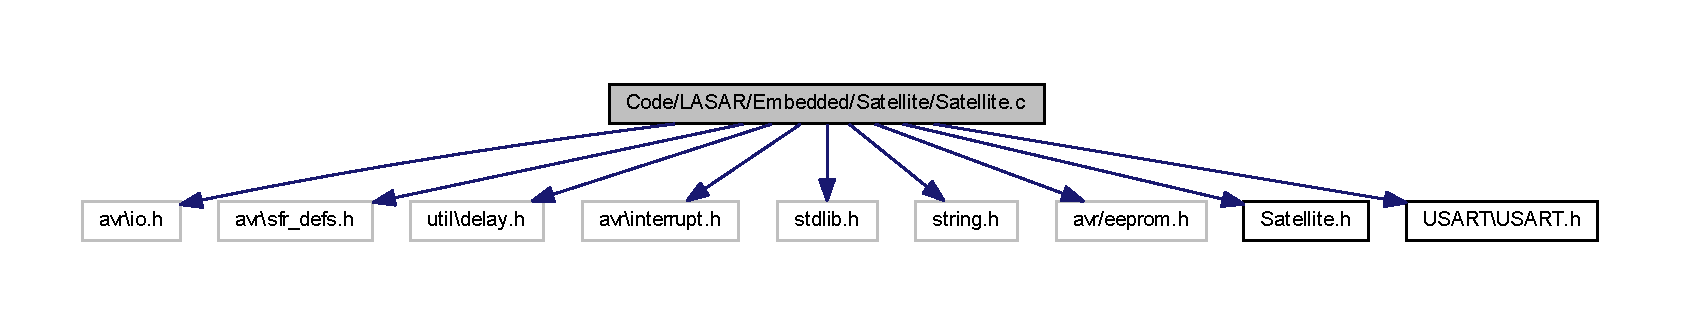
\includegraphics[width=350pt]{_satellite_8c__incl}
\end{center}
\end{figure}
\subsection*{Functions}
\begin{DoxyCompactItemize}
\item 
int \hyperlink{_satellite_8c_a840291bc02cba5474a4cb46a9b9566fe}{main} (void)
\item 
void \hyperlink{_satellite_8c_a1f576ee1d06e908fc16330a4506780a9}{check\-Alarm} ()
\begin{DoxyCompactList}\small\item\em Check current time vs alarm times Checks the hour of an alarm. If true, it then checks the minutes. \end{DoxyCompactList}\item 
void \hyperlink{_satellite_8c_a3f325a8aec708de6a186e6268f38d045}{set\-Dim} (int arg)
\begin{DoxyCompactList}\small\item\em Set current Dim Value Provides a central function to call in order to change the value. N\-O\-T\-E\-: This {\bfseries does} change the brightness level. \end{DoxyCompactList}\item 
void \hyperlink{_satellite_8c_a7fbfa2cedde30ed04396cc0a3f232f59}{set\-Blinds} (int arg)
\begin{DoxyCompactList}\small\item\em Set current Blinds value Provides a central function to call in order to change the value. N\-O\-T\-E\-: Does {\bfseries not} change the blinds level. \end{DoxyCompactList}\item 
uint8\-\_\-t \hyperlink{_satellite_8c_a11e0fd7642e9f27565483c004bfbadd7}{get\-Digits} (char $\ast$cmd, uint8\-\_\-t $\ast$i)
\begin{DoxyCompactList}\small\item\em Modified atoi Parses the command string for integer values. \end{DoxyCompactList}\item 
void \hyperlink{_satellite_8c_ac3f87e7d8ba1b0dbacfd1bc1674cb92c}{check\-P\-I\-R} ()
\begin{DoxyCompactList}\small\item\em Monitor any movement registered by P\-I\-R sensor In the even of motion, the P\-I\-R data line will be high. The line is debounced in order to not receive noise. \end{DoxyCompactList}\item 
void \hyperlink{_satellite_8c_af0309a165c5eb3e860fd75ce362b8529}{init\-A\-C} (int dutycycle)
\begin{DoxyCompactList}\small\item\em Initializes A\-C light control Declares timer settings and starts the timer Initializes the interrupt values specific to the phase control. \end{DoxyCompactList}\item 
void \hyperlink{_satellite_8c_a2f78b3f3318ab9a0a24a164f24256268}{init\-L2\-F} ()
\begin{DoxyCompactList}\small\item\em Initializes Light to Frequency Converter Sets the proper interrupt values for P\-C\-I\-N\-T20. This uses the same timer as the P\-I\-R sensor. \end{DoxyCompactList}\item 
void \hyperlink{_satellite_8c_a228ca26c149b48d0fa6a9e3c2c7975d0}{init\-P\-I\-R} ()
\begin{DoxyCompactList}\small\item\em Initialize Personal Infrared Sensor Sets the proper interrupt values for P\-C\-I\-N\-T0. \end{DoxyCompactList}\item 
void \hyperlink{_satellite_8c_a7f03a61277bace0b0331e42497e0b69c}{init\-Servo} ()
\begin{DoxyCompactList}\small\item\em Initialize Servos that control Blinds A nice hack that uses a smaller, 8-\/bit timer to do the work usually relegated to a 16-\/bit timer. \end{DoxyCompactList}\item 
static void \hyperlink{_satellite_8c_a21eb55c2ad090fd3041505a5a09898e5}{vary\-Blinds} (int8\-\_\-t percent)
\begin{DoxyCompactList}\small\item\em Open/\-Close Blinds Calculates the amount of time to open or close the blinds. Sign value of the percentage decides servo direction. Positive percentage moves forward, negative backward. \end{DoxyCompactList}\item 
\hyperlink{_satellite_8c_a9c4665742c6b6eb1f0bb9dde41f7cba3}{I\-S\-R} (P\-C\-I\-N\-T2\-\_\-vect)
\begin{DoxyCompactList}\small\item\em Light to Frequency Detection If the L2\-F sensor has pulsed high, we increment the Num\-Changes variable. \end{DoxyCompactList}\item 
\hyperlink{_satellite_8c_a09ce999e15ad60b8a3f07d08af1946f9}{I\-S\-R} (U\-S\-A\-R\-T\-\_\-\-R\-X\-\_\-vect)
\begin{DoxyCompactList}\small\item\em Bluetooth Receive Receives a string from the Bluetooth module. Relies on ';' terminator. \end{DoxyCompactList}\item 
\hyperlink{_satellite_8c_aec43762dc86e029b395d4e5819192c2d}{I\-S\-R} (T\-I\-M\-E\-R0\-\_\-\-C\-O\-M\-P\-A\-\_\-vect)
\begin{DoxyCompactList}\small\item\em A\-C Lighting Control C\-R\-E\-A\-T\-E\-D\-: 2/15/2012. \end{DoxyCompactList}\item 
\hyperlink{_satellite_8c_ad39420cdd896dd12c68e36313139d0a5}{I\-S\-R} (T\-I\-M\-E\-R1\-\_\-\-C\-O\-M\-P\-A\-\_\-vect)
\begin{DoxyCompactList}\small\item\em 1\-Hz Timer Every second, the microcontroller performs the Light to Frequency calculation. If the P\-I\-R sensor hasn't sensed any movement, the t\-Inactive variable is also incremented. \end{DoxyCompactList}\item 
\hyperlink{_satellite_8c_a5686c229bdef50123688ab6cb1404230}{I\-S\-R} (T\-I\-M\-E\-R2\-\_\-\-C\-O\-M\-P\-A\-\_\-vect)
\begin{DoxyCompactList}\small\item\em Timer 2 Compare When the timer has achieved the proper P\-W\-M value, set the Servo data line low. \end{DoxyCompactList}\item 
\hyperlink{_satellite_8c_a7cfcbe42bd266750aeb6e5d71e5ea479}{I\-S\-R} (T\-I\-M\-E\-R2\-\_\-\-O\-V\-F\-\_\-vect)
\begin{DoxyCompactList}\small\item\em Timer 2 Overflow for Servo Control Sets the Servo data pin high when timer has reverted to 0. \end{DoxyCompactList}\item 
\hyperlink{_satellite_8c_afea150fcd685610cb9f7672fce361e53}{I\-S\-R} (I\-N\-T0\-\_\-vect)
\begin{DoxyCompactList}\small\item\em A\-C -\/ Zero Cross Detection. \end{DoxyCompactList}\item 
\hyperlink{_satellite_8c_a0c4271458583c66d6662599d7489194f}{I\-S\-R} (\-\_\-\-\_\-vector\-\_\-default)
\begin{DoxyCompactList}\small\item\em Prevents Microcontroller from resetting. \end{DoxyCompactList}\item 
static void \hyperlink{_satellite_8c_a0ab136e9ebd2b5d9caae63438d058188}{delay\-\_\-ms} (uint16\-\_\-t tick)
\begin{DoxyCompactList}\small\item\em Allows for dynamic delay. \end{DoxyCompactList}\end{DoxyCompactItemize}
\subsection*{Variables}
\begin{DoxyCompactItemize}
\item 
volatile uint8\-\_\-t \hyperlink{_satellite_8c_a236f770a65f752918757c3958cf5f204}{rxflag} = 0
\item 
volatile uint8\-\_\-t \hyperlink{_satellite_8c_aae650fce085d4bfa870f43ff053964ae}{received} = 0
\item 
volatile char \hyperlink{_satellite_8c_a26575f218c319e03f9e581961d0db951}{command} \mbox{[}15\mbox{]}
\item 
volatile uint8\-\_\-t \hyperlink{_satellite_8c_abd869966ad1fb32842901995c490a5c1}{set} = 1
\item 
volatile int \hyperlink{_satellite_8c_a2f56caf41aa76b051430902e2fa4ed0a}{dim}
\item 
volatile int \hyperlink{_satellite_8c_a22c9b1ebd8f3dc707066230c17527163}{tdim}
\item 
volatile unsigned int \hyperlink{_satellite_8c_a77fea233825d3ea077bf940956640746}{count} = 0
\item 
volatile uint8\-\_\-t \hyperlink{_satellite_8c_a44a37c71a87f51f50552afb1c9a858a0}{zerocross} = 0
\item 
volatile int8\-\_\-t \hyperlink{_satellite_8c_a1bf7d853caa0838f152723bfe86a953a}{blinds}
\item 
volatile uint8\-\_\-t \hyperlink{_satellite_8c_a45b83f9bb83b05404aef1d255b8e7beb}{s\-Active} = 0
\item 
volatile uint8\-\_\-t \hyperlink{_satellite_8c_aaca88a07087bab2b9d497ead6054f9e2}{active} = 1
\item 
volatile uint8\-\_\-t \hyperlink{_satellite_8c_ab319800be110c80687e8dabcd09f411c}{t\-Inactive} = 0
\item 
volatile unsigned long \hyperlink{_satellite_8c_aa91412b6d4211cd461707df577a1b5ef}{Num\-Changes} = 0
\item 
volatile float \hyperlink{_satellite_8c_abb0c4079531ec692220077cfa80e1c68}{Freq} = 0
\item 
volatile int \hyperlink{_satellite_8c_af7bb98cfb642794e39ce4069aaa8de27}{d1}
\item 
volatile int \hyperlink{_satellite_8c_a3262002a0b06dd6387fb8944fd89daa0}{d2}
\item 
uint8\-\_\-t \hyperlink{_satellite_8c_ad6a84f4aa9d151edcaa73ee23c0974f2}{chour} = 8
\item 
uint8\-\_\-t \hyperlink{_satellite_8c_ac4aa070aa10b8e9b4030f4180b583a7d}{cmin} = 00
\item 
uint8\-\_\-t \hyperlink{_satellite_8c_a35012c650dea927c17f796823e3ae55f}{csec} = 00
\item 
\hyperlink{struct_pref}{Pref} E\-E\-M\-E\-M \hyperlink{_satellite_8c_a5af3723c41140b2caccbf79a50051919}{wake}
\item 
\hyperlink{struct_pref}{Pref} E\-E\-M\-E\-M \hyperlink{_satellite_8c_a44ab544c3240a2ef9c9e450af43920c8}{leave}
\item 
\hyperlink{struct_pref}{Pref} E\-E\-M\-E\-M \hyperlink{_satellite_8c_a233d61594d9ce03f4c281f689824ba9d}{sleep}
\item 
\hyperlink{struct_pref}{Pref} E\-E\-M\-E\-M \hyperlink{_satellite_8c_af3ec09938eae73bb89a737cf21f8df84}{ret}
\item 
uint8\-\_\-t E\-E\-M\-E\-M \hyperlink{_satellite_8c_add9b652df57b49cbba197653f59e4229}{s\-Blinds} = 0
\item 
uint8\-\_\-t E\-E\-M\-E\-M \hyperlink{_satellite_8c_abaf22b1154093cac603e7ceba1f9803d}{s\-Dim} = 0
\end{DoxyCompactItemize}


\subsection{Function Documentation}
\hypertarget{_satellite_8c_a1f576ee1d06e908fc16330a4506780a9}{\index{Satellite.\-c@{Satellite.\-c}!check\-Alarm@{check\-Alarm}}
\index{check\-Alarm@{check\-Alarm}!Satellite.c@{Satellite.\-c}}
\subsubsection[{check\-Alarm}]{\setlength{\rightskip}{0pt plus 5cm}void {\bf check\-Alarm} (
\begin{DoxyParamCaption}
{}
\end{DoxyParamCaption}
)}}\label{_satellite_8c_a1f576ee1d06e908fc16330a4506780a9}


Check current time vs alarm times Checks the hour of an alarm. If true, it then checks the minutes. 



Here is the call graph for this function\-:\nopagebreak
\begin{figure}[H]
\begin{center}
\leavevmode
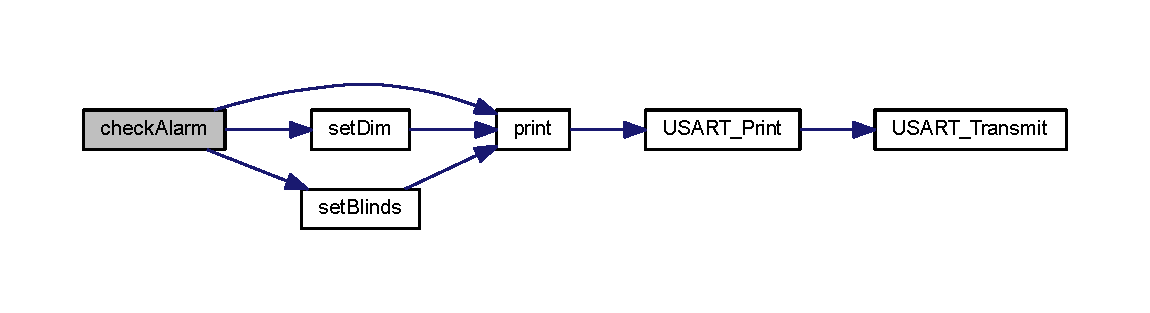
\includegraphics[width=350pt]{_satellite_8c_a1f576ee1d06e908fc16330a4506780a9_cgraph}
\end{center}
\end{figure}




Here is the caller graph for this function\-:\nopagebreak
\begin{figure}[H]
\begin{center}
\leavevmode
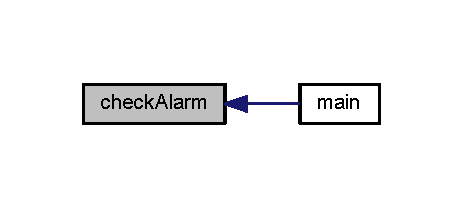
\includegraphics[width=222pt]{_satellite_8c_a1f576ee1d06e908fc16330a4506780a9_icgraph}
\end{center}
\end{figure}


\hypertarget{_satellite_8c_ac3f87e7d8ba1b0dbacfd1bc1674cb92c}{\index{Satellite.\-c@{Satellite.\-c}!check\-P\-I\-R@{check\-P\-I\-R}}
\index{check\-P\-I\-R@{check\-P\-I\-R}!Satellite.c@{Satellite.\-c}}
\subsubsection[{check\-P\-I\-R}]{\setlength{\rightskip}{0pt plus 5cm}void {\bf check\-P\-I\-R} (
\begin{DoxyParamCaption}
{}
\end{DoxyParamCaption}
)}}\label{_satellite_8c_ac3f87e7d8ba1b0dbacfd1bc1674cb92c}


Monitor any movement registered by P\-I\-R sensor In the even of motion, the P\-I\-R data line will be high. The line is debounced in order to not receive noise. 



Here is the call graph for this function\-:\nopagebreak
\begin{figure}[H]
\begin{center}
\leavevmode
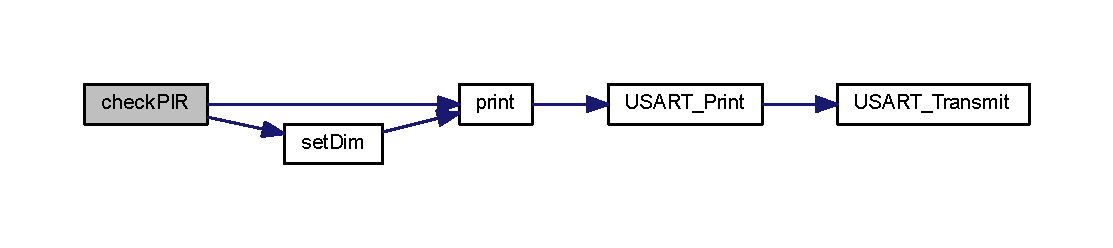
\includegraphics[width=350pt]{_satellite_8c_ac3f87e7d8ba1b0dbacfd1bc1674cb92c_cgraph}
\end{center}
\end{figure}




Here is the caller graph for this function\-:\nopagebreak
\begin{figure}[H]
\begin{center}
\leavevmode
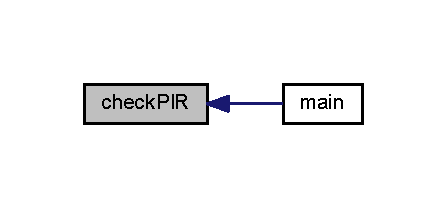
\includegraphics[width=214pt]{_satellite_8c_ac3f87e7d8ba1b0dbacfd1bc1674cb92c_icgraph}
\end{center}
\end{figure}


\hypertarget{_satellite_8c_a0ab136e9ebd2b5d9caae63438d058188}{\index{Satellite.\-c@{Satellite.\-c}!delay\-\_\-ms@{delay\-\_\-ms}}
\index{delay\-\_\-ms@{delay\-\_\-ms}!Satellite.c@{Satellite.\-c}}
\subsubsection[{delay\-\_\-ms}]{\setlength{\rightskip}{0pt plus 5cm}static void {\bf delay\-\_\-ms} (
\begin{DoxyParamCaption}
\item[{uint16\-\_\-t}]{tick}
\end{DoxyParamCaption}
)\hspace{0.3cm}{\ttfamily  \mbox{[}inline, static\mbox{]}}}}\label{_satellite_8c_a0ab136e9ebd2b5d9caae63438d058188}


Allows for dynamic delay. 


\begin{DoxyParams}{Parameters}
{\em tick} & Custom milliseconds to delay \\
\hline
\end{DoxyParams}


Here is the caller graph for this function\-:\nopagebreak
\begin{figure}[H]
\begin{center}
\leavevmode
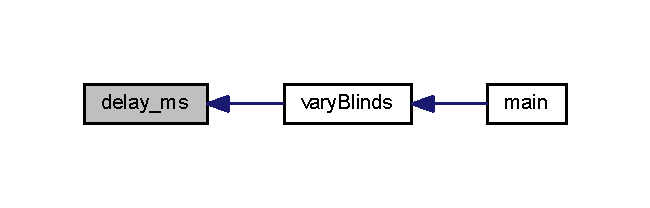
\includegraphics[width=312pt]{_satellite_8c_a0ab136e9ebd2b5d9caae63438d058188_icgraph}
\end{center}
\end{figure}


\hypertarget{_satellite_8c_a11e0fd7642e9f27565483c004bfbadd7}{\index{Satellite.\-c@{Satellite.\-c}!get\-Digits@{get\-Digits}}
\index{get\-Digits@{get\-Digits}!Satellite.c@{Satellite.\-c}}
\subsubsection[{get\-Digits}]{\setlength{\rightskip}{0pt plus 5cm}uint8\-\_\-t {\bf get\-Digits} (
\begin{DoxyParamCaption}
\item[{char $\ast$}]{cmd, }
\item[{uint8\-\_\-t $\ast$}]{i}
\end{DoxyParamCaption}
)}}\label{_satellite_8c_a11e0fd7642e9f27565483c004bfbadd7}


Modified atoi Parses the command string for integer values. 


\begin{DoxyParams}{Parameters}
{\em cmd} & Command string \\
\hline
{\em i} & Length of the entire command string \\
\hline
\end{DoxyParams}
\begin{DoxyReturn}{Returns}
Value parsed 
\end{DoxyReturn}


Here is the caller graph for this function\-:\nopagebreak
\begin{figure}[H]
\begin{center}
\leavevmode
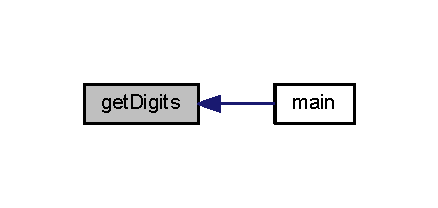
\includegraphics[width=210pt]{_satellite_8c_a11e0fd7642e9f27565483c004bfbadd7_icgraph}
\end{center}
\end{figure}


\hypertarget{_satellite_8c_af0309a165c5eb3e860fd75ce362b8529}{\index{Satellite.\-c@{Satellite.\-c}!init\-A\-C@{init\-A\-C}}
\index{init\-A\-C@{init\-A\-C}!Satellite.c@{Satellite.\-c}}
\subsubsection[{init\-A\-C}]{\setlength{\rightskip}{0pt plus 5cm}void {\bf init\-A\-C} (
\begin{DoxyParamCaption}
\item[{int}]{dutycycle}
\end{DoxyParamCaption}
)}}\label{_satellite_8c_af0309a165c5eb3e860fd75ce362b8529}


Initializes A\-C light control Declares timer settings and starts the timer Initializes the interrupt values specific to the phase control. 


\begin{DoxyParams}{Parameters}
{\em dutycycle} & Duty cycle of A\-C wave \\
\hline
\end{DoxyParams}


Here is the caller graph for this function\-:\nopagebreak
\begin{figure}[H]
\begin{center}
\leavevmode
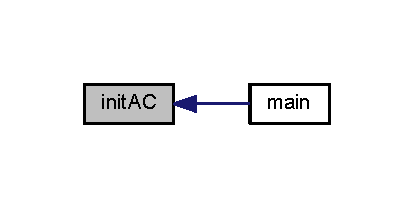
\includegraphics[width=198pt]{_satellite_8c_af0309a165c5eb3e860fd75ce362b8529_icgraph}
\end{center}
\end{figure}


\hypertarget{_satellite_8c_a2f78b3f3318ab9a0a24a164f24256268}{\index{Satellite.\-c@{Satellite.\-c}!init\-L2\-F@{init\-L2\-F}}
\index{init\-L2\-F@{init\-L2\-F}!Satellite.c@{Satellite.\-c}}
\subsubsection[{init\-L2\-F}]{\setlength{\rightskip}{0pt plus 5cm}void {\bf init\-L2\-F} (
\begin{DoxyParamCaption}
{}
\end{DoxyParamCaption}
)}}\label{_satellite_8c_a2f78b3f3318ab9a0a24a164f24256268}


Initializes Light to Frequency Converter Sets the proper interrupt values for P\-C\-I\-N\-T20. This uses the same timer as the P\-I\-R sensor. 



Here is the caller graph for this function\-:\nopagebreak
\begin{figure}[H]
\begin{center}
\leavevmode
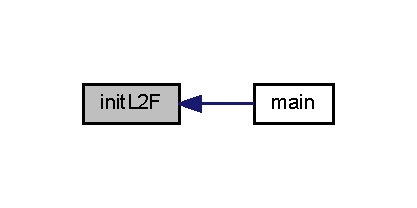
\includegraphics[width=200pt]{_satellite_8c_a2f78b3f3318ab9a0a24a164f24256268_icgraph}
\end{center}
\end{figure}


\hypertarget{_satellite_8c_a228ca26c149b48d0fa6a9e3c2c7975d0}{\index{Satellite.\-c@{Satellite.\-c}!init\-P\-I\-R@{init\-P\-I\-R}}
\index{init\-P\-I\-R@{init\-P\-I\-R}!Satellite.c@{Satellite.\-c}}
\subsubsection[{init\-P\-I\-R}]{\setlength{\rightskip}{0pt plus 5cm}void {\bf init\-P\-I\-R} (
\begin{DoxyParamCaption}
{}
\end{DoxyParamCaption}
)}}\label{_satellite_8c_a228ca26c149b48d0fa6a9e3c2c7975d0}


Initialize Personal Infrared Sensor Sets the proper interrupt values for P\-C\-I\-N\-T0. 



Here is the caller graph for this function\-:\nopagebreak
\begin{figure}[H]
\begin{center}
\leavevmode
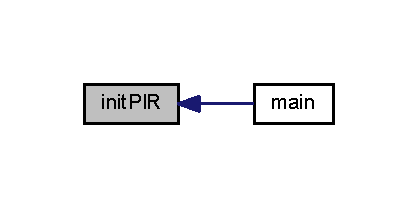
\includegraphics[width=200pt]{_satellite_8c_a228ca26c149b48d0fa6a9e3c2c7975d0_icgraph}
\end{center}
\end{figure}


\hypertarget{_satellite_8c_a7f03a61277bace0b0331e42497e0b69c}{\index{Satellite.\-c@{Satellite.\-c}!init\-Servo@{init\-Servo}}
\index{init\-Servo@{init\-Servo}!Satellite.c@{Satellite.\-c}}
\subsubsection[{init\-Servo}]{\setlength{\rightskip}{0pt plus 5cm}void {\bf init\-Servo} (
\begin{DoxyParamCaption}
{}
\end{DoxyParamCaption}
)}}\label{_satellite_8c_a7f03a61277bace0b0331e42497e0b69c}


Initialize Servos that control Blinds A nice hack that uses a smaller, 8-\/bit timer to do the work usually relegated to a 16-\/bit timer. 

$<$ Prescalar /1024

$<$ Enable O\-V\-F 

Here is the caller graph for this function\-:\nopagebreak
\begin{figure}[H]
\begin{center}
\leavevmode
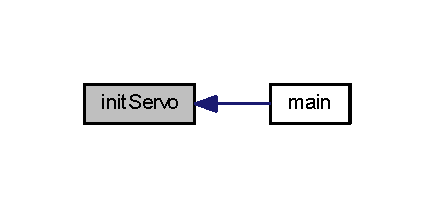
\includegraphics[width=208pt]{_satellite_8c_a7f03a61277bace0b0331e42497e0b69c_icgraph}
\end{center}
\end{figure}


\hypertarget{_satellite_8c_a9c4665742c6b6eb1f0bb9dde41f7cba3}{\index{Satellite.\-c@{Satellite.\-c}!I\-S\-R@{I\-S\-R}}
\index{I\-S\-R@{I\-S\-R}!Satellite.c@{Satellite.\-c}}
\subsubsection[{I\-S\-R}]{\setlength{\rightskip}{0pt plus 5cm}{\bf I\-S\-R} (
\begin{DoxyParamCaption}
\item[{P\-C\-I\-N\-T2\-\_\-vect}]{}
\end{DoxyParamCaption}
)}}\label{_satellite_8c_a9c4665742c6b6eb1f0bb9dde41f7cba3}


Light to Frequency Detection If the L2\-F sensor has pulsed high, we increment the Num\-Changes variable. 

\hypertarget{_satellite_8c_a09ce999e15ad60b8a3f07d08af1946f9}{\index{Satellite.\-c@{Satellite.\-c}!I\-S\-R@{I\-S\-R}}
\index{I\-S\-R@{I\-S\-R}!Satellite.c@{Satellite.\-c}}
\subsubsection[{I\-S\-R}]{\setlength{\rightskip}{0pt plus 5cm}{\bf I\-S\-R} (
\begin{DoxyParamCaption}
\item[{U\-S\-A\-R\-T\-\_\-\-R\-X\-\_\-vect}]{}
\end{DoxyParamCaption}
)}}\label{_satellite_8c_a09ce999e15ad60b8a3f07d08af1946f9}


Bluetooth Receive Receives a string from the Bluetooth module. Relies on ';' terminator. 



Here is the call graph for this function\-:\nopagebreak
\begin{figure}[H]
\begin{center}
\leavevmode
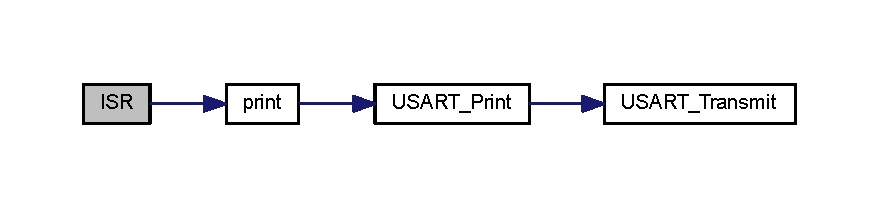
\includegraphics[width=350pt]{_satellite_8c_a09ce999e15ad60b8a3f07d08af1946f9_cgraph}
\end{center}
\end{figure}


\hypertarget{_satellite_8c_aec43762dc86e029b395d4e5819192c2d}{\index{Satellite.\-c@{Satellite.\-c}!I\-S\-R@{I\-S\-R}}
\index{I\-S\-R@{I\-S\-R}!Satellite.c@{Satellite.\-c}}
\subsubsection[{I\-S\-R}]{\setlength{\rightskip}{0pt plus 5cm}{\bf I\-S\-R} (
\begin{DoxyParamCaption}
\item[{T\-I\-M\-E\-R0\-\_\-\-C\-O\-M\-P\-A\-\_\-vect}]{}
\end{DoxyParamCaption}
)}}\label{_satellite_8c_aec43762dc86e029b395d4e5819192c2d}


A\-C Lighting Control C\-R\-E\-A\-T\-E\-D\-: 2/15/2012. 

\hypertarget{_satellite_8c_ad39420cdd896dd12c68e36313139d0a5}{\index{Satellite.\-c@{Satellite.\-c}!I\-S\-R@{I\-S\-R}}
\index{I\-S\-R@{I\-S\-R}!Satellite.c@{Satellite.\-c}}
\subsubsection[{I\-S\-R}]{\setlength{\rightskip}{0pt plus 5cm}{\bf I\-S\-R} (
\begin{DoxyParamCaption}
\item[{T\-I\-M\-E\-R1\-\_\-\-C\-O\-M\-P\-A\-\_\-vect}]{}
\end{DoxyParamCaption}
)}}\label{_satellite_8c_ad39420cdd896dd12c68e36313139d0a5}


1\-Hz Timer Every second, the microcontroller performs the Light to Frequency calculation. If the P\-I\-R sensor hasn't sensed any movement, the t\-Inactive variable is also incremented. 

\hypertarget{_satellite_8c_a5686c229bdef50123688ab6cb1404230}{\index{Satellite.\-c@{Satellite.\-c}!I\-S\-R@{I\-S\-R}}
\index{I\-S\-R@{I\-S\-R}!Satellite.c@{Satellite.\-c}}
\subsubsection[{I\-S\-R}]{\setlength{\rightskip}{0pt plus 5cm}{\bf I\-S\-R} (
\begin{DoxyParamCaption}
\item[{T\-I\-M\-E\-R2\-\_\-\-C\-O\-M\-P\-A\-\_\-vect}]{}
\end{DoxyParamCaption}
)}}\label{_satellite_8c_a5686c229bdef50123688ab6cb1404230}


Timer 2 Compare When the timer has achieved the proper P\-W\-M value, set the Servo data line low. 

\hypertarget{_satellite_8c_a7cfcbe42bd266750aeb6e5d71e5ea479}{\index{Satellite.\-c@{Satellite.\-c}!I\-S\-R@{I\-S\-R}}
\index{I\-S\-R@{I\-S\-R}!Satellite.c@{Satellite.\-c}}
\subsubsection[{I\-S\-R}]{\setlength{\rightskip}{0pt plus 5cm}{\bf I\-S\-R} (
\begin{DoxyParamCaption}
\item[{T\-I\-M\-E\-R2\-\_\-\-O\-V\-F\-\_\-vect}]{}
\end{DoxyParamCaption}
)}}\label{_satellite_8c_a7cfcbe42bd266750aeb6e5d71e5ea479}


Timer 2 Overflow for Servo Control Sets the Servo data pin high when timer has reverted to 0. 

\hypertarget{_satellite_8c_afea150fcd685610cb9f7672fce361e53}{\index{Satellite.\-c@{Satellite.\-c}!I\-S\-R@{I\-S\-R}}
\index{I\-S\-R@{I\-S\-R}!Satellite.c@{Satellite.\-c}}
\subsubsection[{I\-S\-R}]{\setlength{\rightskip}{0pt plus 5cm}{\bf I\-S\-R} (
\begin{DoxyParamCaption}
\item[{I\-N\-T0\-\_\-vect}]{}
\end{DoxyParamCaption}
)}}\label{_satellite_8c_afea150fcd685610cb9f7672fce361e53}


A\-C -\/ Zero Cross Detection. 

\hypertarget{_satellite_8c_a0c4271458583c66d6662599d7489194f}{\index{Satellite.\-c@{Satellite.\-c}!I\-S\-R@{I\-S\-R}}
\index{I\-S\-R@{I\-S\-R}!Satellite.c@{Satellite.\-c}}
\subsubsection[{I\-S\-R}]{\setlength{\rightskip}{0pt plus 5cm}{\bf I\-S\-R} (
\begin{DoxyParamCaption}
\item[{\-\_\-\-\_\-vector\-\_\-default}]{}
\end{DoxyParamCaption}
)}}\label{_satellite_8c_a0c4271458583c66d6662599d7489194f}


Prevents Microcontroller from resetting. 

\hypertarget{_satellite_8c_a840291bc02cba5474a4cb46a9b9566fe}{\index{Satellite.\-c@{Satellite.\-c}!main@{main}}
\index{main@{main}!Satellite.c@{Satellite.\-c}}
\subsubsection[{main}]{\setlength{\rightskip}{0pt plus 5cm}int {\bf main} (
\begin{DoxyParamCaption}
\item[{void}]{}
\end{DoxyParamCaption}
)}}\label{_satellite_8c_a840291bc02cba5474a4cb46a9b9566fe}


Here is the call graph for this function\-:\nopagebreak
\begin{figure}[H]
\begin{center}
\leavevmode
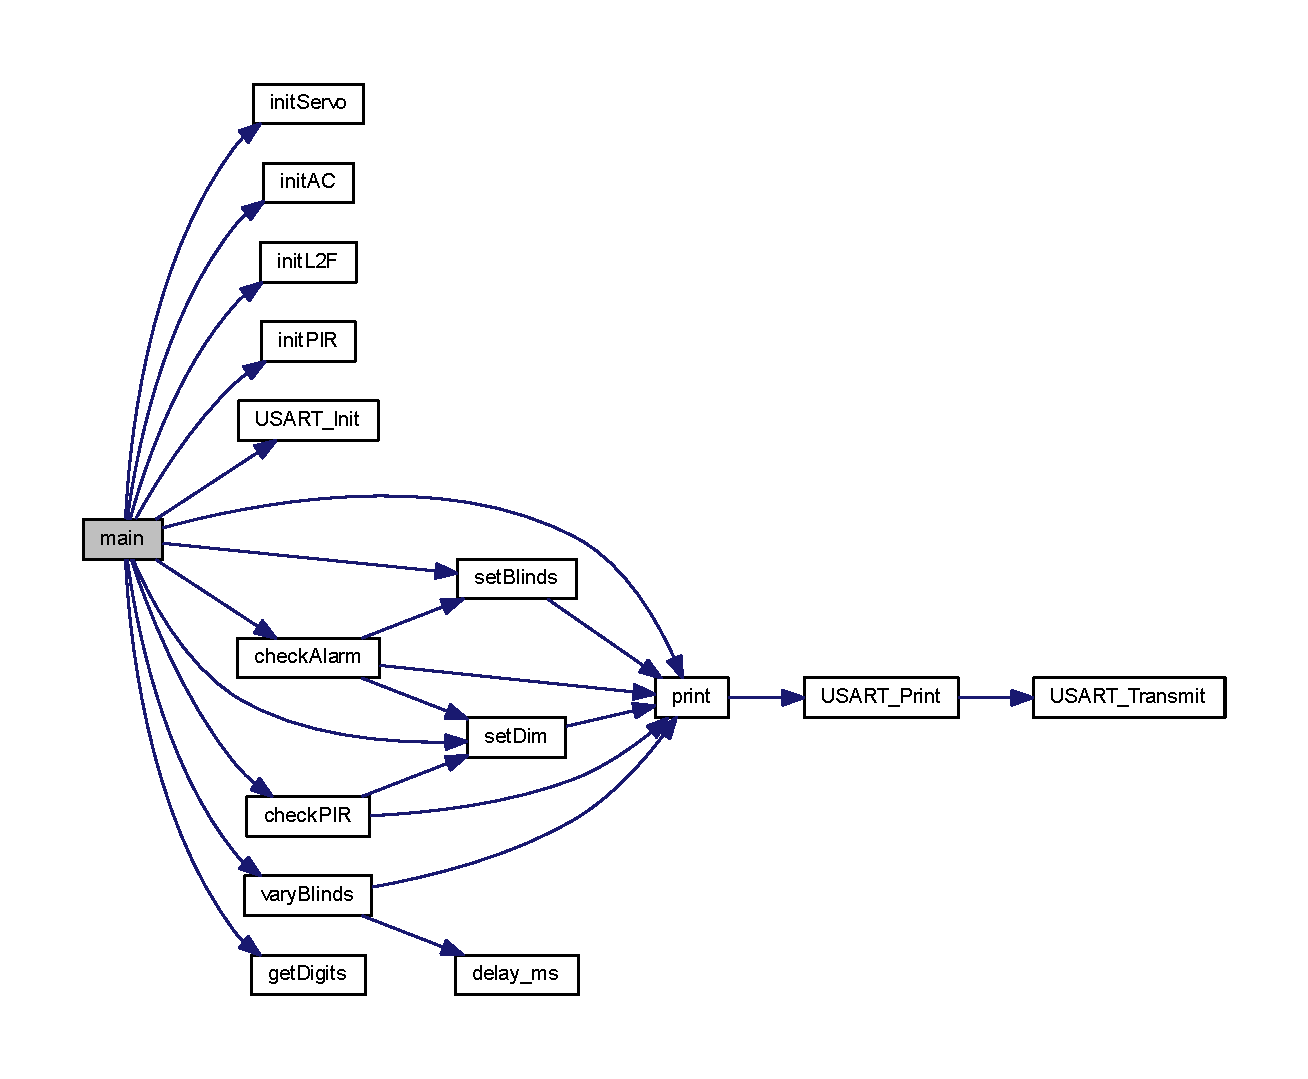
\includegraphics[width=350pt]{_satellite_8c_a840291bc02cba5474a4cb46a9b9566fe_cgraph}
\end{center}
\end{figure}


\hypertarget{_satellite_8c_a7fbfa2cedde30ed04396cc0a3f232f59}{\index{Satellite.\-c@{Satellite.\-c}!set\-Blinds@{set\-Blinds}}
\index{set\-Blinds@{set\-Blinds}!Satellite.c@{Satellite.\-c}}
\subsubsection[{set\-Blinds}]{\setlength{\rightskip}{0pt plus 5cm}void {\bf set\-Blinds} (
\begin{DoxyParamCaption}
\item[{int}]{arg}
\end{DoxyParamCaption}
)}}\label{_satellite_8c_a7fbfa2cedde30ed04396cc0a3f232f59}


Set current Blinds value Provides a central function to call in order to change the value. N\-O\-T\-E\-: Does {\bfseries not} change the blinds level. 


\begin{DoxyParams}{Parameters}
{\em arg} & Percent difference that blinds must be set to \\
\hline
\end{DoxyParams}
\begin{DoxyReturn}{Returns}
Whether the move has been performed 
\end{DoxyReturn}


Here is the call graph for this function\-:\nopagebreak
\begin{figure}[H]
\begin{center}
\leavevmode
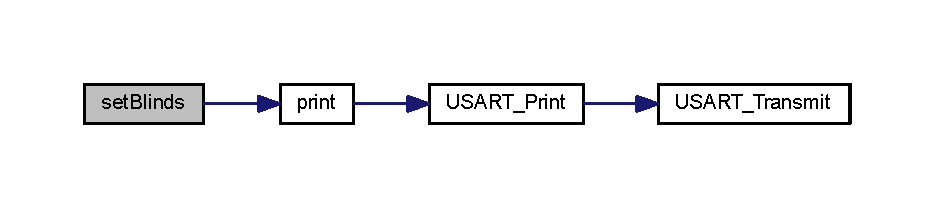
\includegraphics[width=350pt]{_satellite_8c_a7fbfa2cedde30ed04396cc0a3f232f59_cgraph}
\end{center}
\end{figure}




Here is the caller graph for this function\-:\nopagebreak
\begin{figure}[H]
\begin{center}
\leavevmode
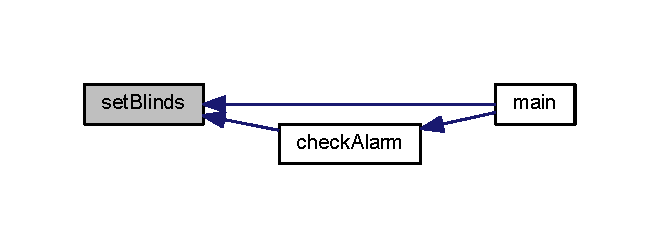
\includegraphics[width=316pt]{_satellite_8c_a7fbfa2cedde30ed04396cc0a3f232f59_icgraph}
\end{center}
\end{figure}


\hypertarget{_satellite_8c_a3f325a8aec708de6a186e6268f38d045}{\index{Satellite.\-c@{Satellite.\-c}!set\-Dim@{set\-Dim}}
\index{set\-Dim@{set\-Dim}!Satellite.c@{Satellite.\-c}}
\subsubsection[{set\-Dim}]{\setlength{\rightskip}{0pt plus 5cm}void {\bf set\-Dim} (
\begin{DoxyParamCaption}
\item[{int}]{arg}
\end{DoxyParamCaption}
)}}\label{_satellite_8c_a3f325a8aec708de6a186e6268f38d045}


Set current Dim Value Provides a central function to call in order to change the value. N\-O\-T\-E\-: This {\bfseries does} change the brightness level. 


\begin{DoxyParams}{Parameters}
{\em arg} & The new brightness level \\
\hline
\end{DoxyParams}
\begin{DoxyReturn}{Returns}
Whether the move has been performed 
\end{DoxyReturn}


Here is the call graph for this function\-:\nopagebreak
\begin{figure}[H]
\begin{center}
\leavevmode
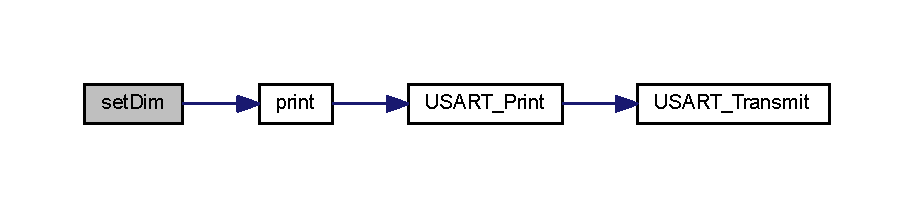
\includegraphics[width=350pt]{_satellite_8c_a3f325a8aec708de6a186e6268f38d045_cgraph}
\end{center}
\end{figure}




Here is the caller graph for this function\-:\nopagebreak
\begin{figure}[H]
\begin{center}
\leavevmode
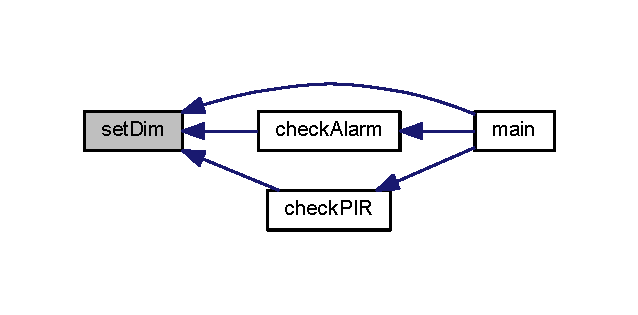
\includegraphics[width=306pt]{_satellite_8c_a3f325a8aec708de6a186e6268f38d045_icgraph}
\end{center}
\end{figure}


\hypertarget{_satellite_8c_a21eb55c2ad090fd3041505a5a09898e5}{\index{Satellite.\-c@{Satellite.\-c}!vary\-Blinds@{vary\-Blinds}}
\index{vary\-Blinds@{vary\-Blinds}!Satellite.c@{Satellite.\-c}}
\subsubsection[{vary\-Blinds}]{\setlength{\rightskip}{0pt plus 5cm}static void {\bf vary\-Blinds} (
\begin{DoxyParamCaption}
\item[{int8\-\_\-t}]{percent}
\end{DoxyParamCaption}
)\hspace{0.3cm}{\ttfamily  \mbox{[}static\mbox{]}}}}\label{_satellite_8c_a21eb55c2ad090fd3041505a5a09898e5}


Open/\-Close Blinds Calculates the amount of time to open or close the blinds. Sign value of the percentage decides servo direction. Positive percentage moves forward, negative backward. 


\begin{DoxyParams}{Parameters}
{\em percent} & Amount to open/close blinds \\
\hline
\end{DoxyParams}


Here is the call graph for this function\-:\nopagebreak
\begin{figure}[H]
\begin{center}
\leavevmode
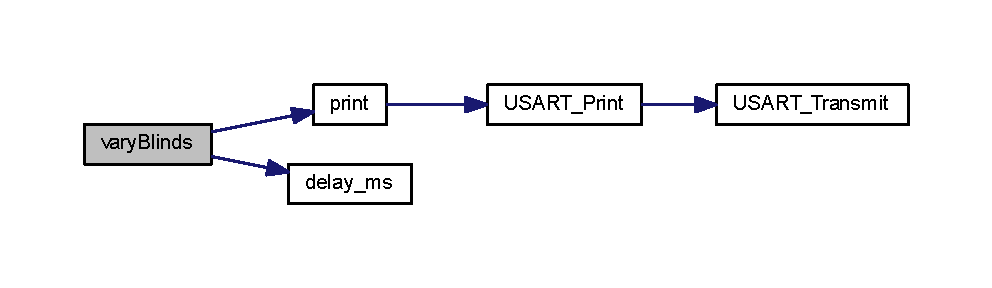
\includegraphics[width=350pt]{_satellite_8c_a21eb55c2ad090fd3041505a5a09898e5_cgraph}
\end{center}
\end{figure}




Here is the caller graph for this function\-:\nopagebreak
\begin{figure}[H]
\begin{center}
\leavevmode
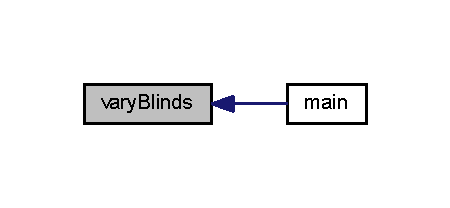
\includegraphics[width=216pt]{_satellite_8c_a21eb55c2ad090fd3041505a5a09898e5_icgraph}
\end{center}
\end{figure}




\subsection{Variable Documentation}
\hypertarget{_satellite_8c_aaca88a07087bab2b9d497ead6054f9e2}{\index{Satellite.\-c@{Satellite.\-c}!active@{active}}
\index{active@{active}!Satellite.c@{Satellite.\-c}}
\subsubsection[{active}]{\setlength{\rightskip}{0pt plus 5cm}volatile uint8\-\_\-t {\bf active} = 1}}\label{_satellite_8c_aaca88a07087bab2b9d497ead6054f9e2}
Flag to indicate if system is active \hypertarget{_satellite_8c_a1bf7d853caa0838f152723bfe86a953a}{\index{Satellite.\-c@{Satellite.\-c}!blinds@{blinds}}
\index{blinds@{blinds}!Satellite.c@{Satellite.\-c}}
\subsubsection[{blinds}]{\setlength{\rightskip}{0pt plus 5cm}volatile int8\-\_\-t {\bf blinds}}}\label{_satellite_8c_a1bf7d853caa0838f152723bfe86a953a}
Blinds open level \hypertarget{_satellite_8c_ad6a84f4aa9d151edcaa73ee23c0974f2}{\index{Satellite.\-c@{Satellite.\-c}!chour@{chour}}
\index{chour@{chour}!Satellite.c@{Satellite.\-c}}
\subsubsection[{chour}]{\setlength{\rightskip}{0pt plus 5cm}uint8\-\_\-t {\bf chour} = 8}}\label{_satellite_8c_ad6a84f4aa9d151edcaa73ee23c0974f2}
Current Hour \hypertarget{_satellite_8c_ac4aa070aa10b8e9b4030f4180b583a7d}{\index{Satellite.\-c@{Satellite.\-c}!cmin@{cmin}}
\index{cmin@{cmin}!Satellite.c@{Satellite.\-c}}
\subsubsection[{cmin}]{\setlength{\rightskip}{0pt plus 5cm}uint8\-\_\-t {\bf cmin} = 00}}\label{_satellite_8c_ac4aa070aa10b8e9b4030f4180b583a7d}
Current Minutes \hypertarget{_satellite_8c_a26575f218c319e03f9e581961d0db951}{\index{Satellite.\-c@{Satellite.\-c}!command@{command}}
\index{command@{command}!Satellite.c@{Satellite.\-c}}
\subsubsection[{command}]{\setlength{\rightskip}{0pt plus 5cm}volatile char {\bf command}\mbox{[}15\mbox{]}}}\label{_satellite_8c_a26575f218c319e03f9e581961d0db951}
Full Command string from Android \hypertarget{_satellite_8c_a77fea233825d3ea077bf940956640746}{\index{Satellite.\-c@{Satellite.\-c}!count@{count}}
\index{count@{count}!Satellite.c@{Satellite.\-c}}
\subsubsection[{count}]{\setlength{\rightskip}{0pt plus 5cm}volatile unsigned int {\bf count} = 0}}\label{_satellite_8c_a77fea233825d3ea077bf940956640746}
Compares this value vs dim to achieve proper delay \hypertarget{_satellite_8c_a35012c650dea927c17f796823e3ae55f}{\index{Satellite.\-c@{Satellite.\-c}!csec@{csec}}
\index{csec@{csec}!Satellite.c@{Satellite.\-c}}
\subsubsection[{csec}]{\setlength{\rightskip}{0pt plus 5cm}uint8\-\_\-t {\bf csec} = 00}}\label{_satellite_8c_a35012c650dea927c17f796823e3ae55f}
Current Seconds \hypertarget{_satellite_8c_af7bb98cfb642794e39ce4069aaa8de27}{\index{Satellite.\-c@{Satellite.\-c}!d1@{d1}}
\index{d1@{d1}!Satellite.c@{Satellite.\-c}}
\subsubsection[{d1}]{\setlength{\rightskip}{0pt plus 5cm}volatile int {\bf d1}}}\label{_satellite_8c_af7bb98cfb642794e39ce4069aaa8de27}
Thousands of Num\-Changes \hypertarget{_satellite_8c_a3262002a0b06dd6387fb8944fd89daa0}{\index{Satellite.\-c@{Satellite.\-c}!d2@{d2}}
\index{d2@{d2}!Satellite.c@{Satellite.\-c}}
\subsubsection[{d2}]{\setlength{\rightskip}{0pt plus 5cm}volatile int {\bf d2}}}\label{_satellite_8c_a3262002a0b06dd6387fb8944fd89daa0}
Hundreds of Num\-Changes \hypertarget{_satellite_8c_a2f56caf41aa76b051430902e2fa4ed0a}{\index{Satellite.\-c@{Satellite.\-c}!dim@{dim}}
\index{dim@{dim}!Satellite.c@{Satellite.\-c}}
\subsubsection[{dim}]{\setlength{\rightskip}{0pt plus 5cm}volatile int {\bf dim}}}\label{_satellite_8c_a2f56caf41aa76b051430902e2fa4ed0a}
A\-C Lighting brightness \hypertarget{_satellite_8c_abb0c4079531ec692220077cfa80e1c68}{\index{Satellite.\-c@{Satellite.\-c}!Freq@{Freq}}
\index{Freq@{Freq}!Satellite.c@{Satellite.\-c}}
\subsubsection[{Freq}]{\setlength{\rightskip}{0pt plus 5cm}volatile float {\bf Freq} = 0}}\label{_satellite_8c_abb0c4079531ec692220077cfa80e1c68}
Store the Frequency \hypertarget{_satellite_8c_a44ab544c3240a2ef9c9e450af43920c8}{\index{Satellite.\-c@{Satellite.\-c}!leave@{leave}}
\index{leave@{leave}!Satellite.c@{Satellite.\-c}}
\subsubsection[{leave}]{\setlength{\rightskip}{0pt plus 5cm}{\bf Pref} E\-E\-M\-E\-M {\bf leave}}}\label{_satellite_8c_a44ab544c3240a2ef9c9e450af43920c8}
Leave preferences \hypertarget{_satellite_8c_aa91412b6d4211cd461707df577a1b5ef}{\index{Satellite.\-c@{Satellite.\-c}!Num\-Changes@{Num\-Changes}}
\index{Num\-Changes@{Num\-Changes}!Satellite.c@{Satellite.\-c}}
\subsubsection[{Num\-Changes}]{\setlength{\rightskip}{0pt plus 5cm}volatile unsigned long {\bf Num\-Changes} = 0}}\label{_satellite_8c_aa91412b6d4211cd461707df577a1b5ef}
Counter of Pulses in Each Measurement Period \hypertarget{_satellite_8c_aae650fce085d4bfa870f43ff053964ae}{\index{Satellite.\-c@{Satellite.\-c}!received@{received}}
\index{received@{received}!Satellite.c@{Satellite.\-c}}
\subsubsection[{received}]{\setlength{\rightskip}{0pt plus 5cm}volatile uint8\-\_\-t {\bf received} = 0}}\label{_satellite_8c_aae650fce085d4bfa870f43ff053964ae}
Byte received from buffer \hypertarget{_satellite_8c_af3ec09938eae73bb89a737cf21f8df84}{\index{Satellite.\-c@{Satellite.\-c}!ret@{ret}}
\index{ret@{ret}!Satellite.c@{Satellite.\-c}}
\subsubsection[{ret}]{\setlength{\rightskip}{0pt plus 5cm}{\bf Pref} E\-E\-M\-E\-M {\bf ret}}}\label{_satellite_8c_af3ec09938eae73bb89a737cf21f8df84}
Return preferences \hypertarget{_satellite_8c_a236f770a65f752918757c3958cf5f204}{\index{Satellite.\-c@{Satellite.\-c}!rxflag@{rxflag}}
\index{rxflag@{rxflag}!Satellite.c@{Satellite.\-c}}
\subsubsection[{rxflag}]{\setlength{\rightskip}{0pt plus 5cm}volatile uint8\-\_\-t {\bf rxflag} = 0}}\label{_satellite_8c_a236f770a65f752918757c3958cf5f204}
Flag to indicate command received \hypertarget{_satellite_8c_a45b83f9bb83b05404aef1d255b8e7beb}{\index{Satellite.\-c@{Satellite.\-c}!s\-Active@{s\-Active}}
\index{s\-Active@{s\-Active}!Satellite.c@{Satellite.\-c}}
\subsubsection[{s\-Active}]{\setlength{\rightskip}{0pt plus 5cm}volatile uint8\-\_\-t {\bf s\-Active} = 0}}\label{_satellite_8c_a45b83f9bb83b05404aef1d255b8e7beb}
Flag to prevent Servo from moving while system is inactive \hypertarget{_satellite_8c_add9b652df57b49cbba197653f59e4229}{\index{Satellite.\-c@{Satellite.\-c}!s\-Blinds@{s\-Blinds}}
\index{s\-Blinds@{s\-Blinds}!Satellite.c@{Satellite.\-c}}
\subsubsection[{s\-Blinds}]{\setlength{\rightskip}{0pt plus 5cm}uint8\-\_\-t E\-E\-M\-E\-M {\bf s\-Blinds} = 0}}\label{_satellite_8c_add9b652df57b49cbba197653f59e4229}
Saved Blinds open level \hypertarget{_satellite_8c_abaf22b1154093cac603e7ceba1f9803d}{\index{Satellite.\-c@{Satellite.\-c}!s\-Dim@{s\-Dim}}
\index{s\-Dim@{s\-Dim}!Satellite.c@{Satellite.\-c}}
\subsubsection[{s\-Dim}]{\setlength{\rightskip}{0pt plus 5cm}uint8\-\_\-t E\-E\-M\-E\-M {\bf s\-Dim} = 0}}\label{_satellite_8c_abaf22b1154093cac603e7ceba1f9803d}
Saved brightness level \hypertarget{_satellite_8c_abd869966ad1fb32842901995c490a5c1}{\index{Satellite.\-c@{Satellite.\-c}!set@{set}}
\index{set@{set}!Satellite.c@{Satellite.\-c}}
\subsubsection[{set}]{\setlength{\rightskip}{0pt plus 5cm}volatile uint8\-\_\-t {\bf set} = 1}}\label{_satellite_8c_abd869966ad1fb32842901995c490a5c1}
Flag to indicate if command has been set \hypertarget{_satellite_8c_a233d61594d9ce03f4c281f689824ba9d}{\index{Satellite.\-c@{Satellite.\-c}!sleep@{sleep}}
\index{sleep@{sleep}!Satellite.c@{Satellite.\-c}}
\subsubsection[{sleep}]{\setlength{\rightskip}{0pt plus 5cm}{\bf Pref} E\-E\-M\-E\-M {\bf sleep}}}\label{_satellite_8c_a233d61594d9ce03f4c281f689824ba9d}
Sleep preferences \hypertarget{_satellite_8c_a22c9b1ebd8f3dc707066230c17527163}{\index{Satellite.\-c@{Satellite.\-c}!tdim@{tdim}}
\index{tdim@{tdim}!Satellite.c@{Satellite.\-c}}
\subsubsection[{tdim}]{\setlength{\rightskip}{0pt plus 5cm}volatile int {\bf tdim}}}\label{_satellite_8c_a22c9b1ebd8f3dc707066230c17527163}
\char`\"{}\-Temp Dim\char`\"{} or the previous brightness level \hypertarget{_satellite_8c_ab319800be110c80687e8dabcd09f411c}{\index{Satellite.\-c@{Satellite.\-c}!t\-Inactive@{t\-Inactive}}
\index{t\-Inactive@{t\-Inactive}!Satellite.c@{Satellite.\-c}}
\subsubsection[{t\-Inactive}]{\setlength{\rightskip}{0pt plus 5cm}volatile uint8\-\_\-t {\bf t\-Inactive} = 0}}\label{_satellite_8c_ab319800be110c80687e8dabcd09f411c}
The amount of time the system has been inactive in seconds \hypertarget{_satellite_8c_a5af3723c41140b2caccbf79a50051919}{\index{Satellite.\-c@{Satellite.\-c}!wake@{wake}}
\index{wake@{wake}!Satellite.c@{Satellite.\-c}}
\subsubsection[{wake}]{\setlength{\rightskip}{0pt plus 5cm}{\bf Pref} E\-E\-M\-E\-M {\bf wake}}}\label{_satellite_8c_a5af3723c41140b2caccbf79a50051919}
Wake preferences \hypertarget{_satellite_8c_a44a37c71a87f51f50552afb1c9a858a0}{\index{Satellite.\-c@{Satellite.\-c}!zerocross@{zerocross}}
\index{zerocross@{zerocross}!Satellite.c@{Satellite.\-c}}
\subsubsection[{zerocross}]{\setlength{\rightskip}{0pt plus 5cm}volatile uint8\-\_\-t {\bf zerocross} = 0}}\label{_satellite_8c_a44a37c71a87f51f50552afb1c9a858a0}
Flag to indicate a zero cross on A\-C line 
\hypertarget{_satellite_8h}{\section{Satellite/\-Satellite.h File Reference}
\label{_satellite_8h}\index{Satellite/\-Satellite.\-h@{Satellite/\-Satellite.\-h}}
}
\subsection*{Data Structures}
\begin{DoxyCompactItemize}
\item 
struct \hyperlink{struct_pref}{Pref}
\item 
struct \hyperlink{struct_time}{Time}
\end{DoxyCompactItemize}
\subsection*{Defines}
\begin{DoxyCompactItemize}
\item 
\#define \hyperlink{_satellite_8h_ad72dbcf6d0153db1b8d8a58001feed83}{D\-E\-B\-U\-G}~0
\item 
\#define \hyperlink{_satellite_8h_afb004735ca38de9210e8b8e9e84fcacb}{S\-E\-R\-V\-O\-\_\-\-P\-E\-R\-I\-O\-D}~312
\item 
\#define \hyperlink{_satellite_8h_a496d0a0c60b8d9cb6f759577c310f217}{S\-E\-R\-V\-O\-\_\-\-F\-W\-D}~0x0\-A
\item 
\#define \hyperlink{_satellite_8h_a8c35450502e6060e9b1617139e745883}{S\-E\-R\-V\-O\-\_\-\-R\-E\-V}~0x2\-F
\item 
\#define \hyperlink{_satellite_8h_a1f1b7bda7db3f5e87e41ea51d048224c}{C\-L\-O\-S\-E\-\_\-\-T\-I\-M\-E}~7000
\item 
\#define \hyperlink{_satellite_8h_a392fb874e547e582e9c66a08a1f23326}{M\-A\-X}~25
\item 
\#define \hyperlink{_satellite_8h_a29e413f6725b2ba32d165ffaa35b01e5}{O\-F\-F}~-\/1
\end{DoxyCompactItemize}
\subsection*{Functions}
\begin{DoxyCompactItemize}
\item 
void \hyperlink{_satellite_8h_af0309a165c5eb3e860fd75ce362b8529}{init\-A\-C} (int dutycycle)
\item 
void \hyperlink{_satellite_8h_a2f78b3f3318ab9a0a24a164f24256268}{init\-L2\-F} ()
\item 
void \hyperlink{_satellite_8h_a228ca26c149b48d0fa6a9e3c2c7975d0}{init\-P\-I\-R} ()
\item 
void \hyperlink{_satellite_8h_a1f576ee1d06e908fc16330a4506780a9}{check\-Alarm} ()
\item 
void \hyperlink{_satellite_8h_a3f325a8aec708de6a186e6268f38d045}{set\-Dim} (int arg)
\item 
void \hyperlink{_satellite_8h_a7fbfa2cedde30ed04396cc0a3f232f59}{set\-Blinds} (int arg)
\item 
void \hyperlink{_satellite_8h_ac3f87e7d8ba1b0dbacfd1bc1674cb92c}{check\-P\-I\-R} ()
\item 
void \hyperlink{_satellite_8h_a7f03a61277bace0b0331e42497e0b69c}{init\-Servo} ()
\item 
void \hyperlink{_satellite_8h_a065adbd131fc5f61263a53739d642766}{init\-Timer} (int dutycycle)
\item 
void \hyperlink{_satellite_8h_afd9b09f58917f0e2d14c61b956eba214}{S\-P\-I\-\_\-init} (void)
\item 
char \hyperlink{_satellite_8h_ae7e64ca53a04fe609757c9260dc3791d}{S\-P\-I\-\_\-\-Transmit} (char c\-Data)
\item 
void \hyperlink{_satellite_8h_a478a022a994b38488f713e1a30107b70}{get\-Time} (uint8\-\_\-t $\ast$hours, uint8\-\_\-t $\ast$minutes, uint8\-\_\-t $\ast$seconds)
\item 
uint8\-\_\-t \hyperlink{_satellite_8h_a11e0fd7642e9f27565483c004bfbadd7}{get\-Digits} (char $\ast$cmd, uint8\-\_\-t $\ast$\hyperlink{_light_controller_8c_af27e3188294c2df66d975b74a09c001d}{i})
\end{DoxyCompactItemize}


\subsection{Define Documentation}
\hypertarget{_satellite_8h_a1f1b7bda7db3f5e87e41ea51d048224c}{\index{Satellite.\-h@{Satellite.\-h}!C\-L\-O\-S\-E\-\_\-\-T\-I\-M\-E@{C\-L\-O\-S\-E\-\_\-\-T\-I\-M\-E}}
\index{C\-L\-O\-S\-E\-\_\-\-T\-I\-M\-E@{C\-L\-O\-S\-E\-\_\-\-T\-I\-M\-E}!Satellite.h@{Satellite.\-h}}
\subsubsection[{C\-L\-O\-S\-E\-\_\-\-T\-I\-M\-E}]{\setlength{\rightskip}{0pt plus 5cm}\#define {\bf C\-L\-O\-S\-E\-\_\-\-T\-I\-M\-E}~7000}}\label{_satellite_8h_a1f1b7bda7db3f5e87e41ea51d048224c}
\hypertarget{_satellite_8h_ad72dbcf6d0153db1b8d8a58001feed83}{\index{Satellite.\-h@{Satellite.\-h}!D\-E\-B\-U\-G@{D\-E\-B\-U\-G}}
\index{D\-E\-B\-U\-G@{D\-E\-B\-U\-G}!Satellite.h@{Satellite.\-h}}
\subsubsection[{D\-E\-B\-U\-G}]{\setlength{\rightskip}{0pt plus 5cm}\#define {\bf D\-E\-B\-U\-G}~0}}\label{_satellite_8h_ad72dbcf6d0153db1b8d8a58001feed83}
\hypertarget{_satellite_8h_a392fb874e547e582e9c66a08a1f23326}{\index{Satellite.\-h@{Satellite.\-h}!M\-A\-X@{M\-A\-X}}
\index{M\-A\-X@{M\-A\-X}!Satellite.h@{Satellite.\-h}}
\subsubsection[{M\-A\-X}]{\setlength{\rightskip}{0pt plus 5cm}\#define {\bf M\-A\-X}~25}}\label{_satellite_8h_a392fb874e547e582e9c66a08a1f23326}
\hypertarget{_satellite_8h_a29e413f6725b2ba32d165ffaa35b01e5}{\index{Satellite.\-h@{Satellite.\-h}!O\-F\-F@{O\-F\-F}}
\index{O\-F\-F@{O\-F\-F}!Satellite.h@{Satellite.\-h}}
\subsubsection[{O\-F\-F}]{\setlength{\rightskip}{0pt plus 5cm}\#define {\bf O\-F\-F}~-\/1}}\label{_satellite_8h_a29e413f6725b2ba32d165ffaa35b01e5}
\hypertarget{_satellite_8h_a496d0a0c60b8d9cb6f759577c310f217}{\index{Satellite.\-h@{Satellite.\-h}!S\-E\-R\-V\-O\-\_\-\-F\-W\-D@{S\-E\-R\-V\-O\-\_\-\-F\-W\-D}}
\index{S\-E\-R\-V\-O\-\_\-\-F\-W\-D@{S\-E\-R\-V\-O\-\_\-\-F\-W\-D}!Satellite.h@{Satellite.\-h}}
\subsubsection[{S\-E\-R\-V\-O\-\_\-\-F\-W\-D}]{\setlength{\rightskip}{0pt plus 5cm}\#define {\bf S\-E\-R\-V\-O\-\_\-\-F\-W\-D}~0x0\-A}}\label{_satellite_8h_a496d0a0c60b8d9cb6f759577c310f217}
\hypertarget{_satellite_8h_afb004735ca38de9210e8b8e9e84fcacb}{\index{Satellite.\-h@{Satellite.\-h}!S\-E\-R\-V\-O\-\_\-\-P\-E\-R\-I\-O\-D@{S\-E\-R\-V\-O\-\_\-\-P\-E\-R\-I\-O\-D}}
\index{S\-E\-R\-V\-O\-\_\-\-P\-E\-R\-I\-O\-D@{S\-E\-R\-V\-O\-\_\-\-P\-E\-R\-I\-O\-D}!Satellite.h@{Satellite.\-h}}
\subsubsection[{S\-E\-R\-V\-O\-\_\-\-P\-E\-R\-I\-O\-D}]{\setlength{\rightskip}{0pt plus 5cm}\#define {\bf S\-E\-R\-V\-O\-\_\-\-P\-E\-R\-I\-O\-D}~312}}\label{_satellite_8h_afb004735ca38de9210e8b8e9e84fcacb}
\hypertarget{_satellite_8h_a8c35450502e6060e9b1617139e745883}{\index{Satellite.\-h@{Satellite.\-h}!S\-E\-R\-V\-O\-\_\-\-R\-E\-V@{S\-E\-R\-V\-O\-\_\-\-R\-E\-V}}
\index{S\-E\-R\-V\-O\-\_\-\-R\-E\-V@{S\-E\-R\-V\-O\-\_\-\-R\-E\-V}!Satellite.h@{Satellite.\-h}}
\subsubsection[{S\-E\-R\-V\-O\-\_\-\-R\-E\-V}]{\setlength{\rightskip}{0pt plus 5cm}\#define {\bf S\-E\-R\-V\-O\-\_\-\-R\-E\-V}~0x2\-F}}\label{_satellite_8h_a8c35450502e6060e9b1617139e745883}


\subsection{Function Documentation}
\hypertarget{_satellite_8h_a1f576ee1d06e908fc16330a4506780a9}{\index{Satellite.\-h@{Satellite.\-h}!check\-Alarm@{check\-Alarm}}
\index{check\-Alarm@{check\-Alarm}!Satellite.h@{Satellite.\-h}}
\subsubsection[{check\-Alarm}]{\setlength{\rightskip}{0pt plus 5cm}void {\bf check\-Alarm} (
\begin{DoxyParamCaption}
{}
\end{DoxyParamCaption}
)}}\label{_satellite_8h_a1f576ee1d06e908fc16330a4506780a9}
\hypertarget{_satellite_8h_ac3f87e7d8ba1b0dbacfd1bc1674cb92c}{\index{Satellite.\-h@{Satellite.\-h}!check\-P\-I\-R@{check\-P\-I\-R}}
\index{check\-P\-I\-R@{check\-P\-I\-R}!Satellite.h@{Satellite.\-h}}
\subsubsection[{check\-P\-I\-R}]{\setlength{\rightskip}{0pt plus 5cm}void {\bf check\-P\-I\-R} (
\begin{DoxyParamCaption}
{}
\end{DoxyParamCaption}
)}}\label{_satellite_8h_ac3f87e7d8ba1b0dbacfd1bc1674cb92c}
\hypertarget{_satellite_8h_a11e0fd7642e9f27565483c004bfbadd7}{\index{Satellite.\-h@{Satellite.\-h}!get\-Digits@{get\-Digits}}
\index{get\-Digits@{get\-Digits}!Satellite.h@{Satellite.\-h}}
\subsubsection[{get\-Digits}]{\setlength{\rightskip}{0pt plus 5cm}uint8\-\_\-t {\bf get\-Digits} (
\begin{DoxyParamCaption}
\item[{char $\ast$}]{cmd, }
\item[{uint8\-\_\-t $\ast$}]{i}
\end{DoxyParamCaption}
)}}\label{_satellite_8h_a11e0fd7642e9f27565483c004bfbadd7}
\hypertarget{_satellite_8h_a478a022a994b38488f713e1a30107b70}{\index{Satellite.\-h@{Satellite.\-h}!get\-Time@{get\-Time}}
\index{get\-Time@{get\-Time}!Satellite.h@{Satellite.\-h}}
\subsubsection[{get\-Time}]{\setlength{\rightskip}{0pt plus 5cm}void {\bf get\-Time} (
\begin{DoxyParamCaption}
\item[{uint8\-\_\-t $\ast$}]{hours, }
\item[{uint8\-\_\-t $\ast$}]{minutes, }
\item[{uint8\-\_\-t $\ast$}]{seconds}
\end{DoxyParamCaption}
)}}\label{_satellite_8h_a478a022a994b38488f713e1a30107b70}
\hypertarget{_satellite_8h_af0309a165c5eb3e860fd75ce362b8529}{\index{Satellite.\-h@{Satellite.\-h}!init\-A\-C@{init\-A\-C}}
\index{init\-A\-C@{init\-A\-C}!Satellite.h@{Satellite.\-h}}
\subsubsection[{init\-A\-C}]{\setlength{\rightskip}{0pt plus 5cm}void {\bf init\-A\-C} (
\begin{DoxyParamCaption}
\item[{int}]{dutycycle}
\end{DoxyParamCaption}
)}}\label{_satellite_8h_af0309a165c5eb3e860fd75ce362b8529}
\hypertarget{_satellite_8h_a2f78b3f3318ab9a0a24a164f24256268}{\index{Satellite.\-h@{Satellite.\-h}!init\-L2\-F@{init\-L2\-F}}
\index{init\-L2\-F@{init\-L2\-F}!Satellite.h@{Satellite.\-h}}
\subsubsection[{init\-L2\-F}]{\setlength{\rightskip}{0pt plus 5cm}void {\bf init\-L2\-F} (
\begin{DoxyParamCaption}
{}
\end{DoxyParamCaption}
)}}\label{_satellite_8h_a2f78b3f3318ab9a0a24a164f24256268}
\hypertarget{_satellite_8h_a228ca26c149b48d0fa6a9e3c2c7975d0}{\index{Satellite.\-h@{Satellite.\-h}!init\-P\-I\-R@{init\-P\-I\-R}}
\index{init\-P\-I\-R@{init\-P\-I\-R}!Satellite.h@{Satellite.\-h}}
\subsubsection[{init\-P\-I\-R}]{\setlength{\rightskip}{0pt plus 5cm}void {\bf init\-P\-I\-R} (
\begin{DoxyParamCaption}
{}
\end{DoxyParamCaption}
)}}\label{_satellite_8h_a228ca26c149b48d0fa6a9e3c2c7975d0}
\hypertarget{_satellite_8h_a7f03a61277bace0b0331e42497e0b69c}{\index{Satellite.\-h@{Satellite.\-h}!init\-Servo@{init\-Servo}}
\index{init\-Servo@{init\-Servo}!Satellite.h@{Satellite.\-h}}
\subsubsection[{init\-Servo}]{\setlength{\rightskip}{0pt plus 5cm}void {\bf init\-Servo} (
\begin{DoxyParamCaption}
{}
\end{DoxyParamCaption}
)}}\label{_satellite_8h_a7f03a61277bace0b0331e42497e0b69c}
\hypertarget{_satellite_8h_a065adbd131fc5f61263a53739d642766}{\index{Satellite.\-h@{Satellite.\-h}!init\-Timer@{init\-Timer}}
\index{init\-Timer@{init\-Timer}!Satellite.h@{Satellite.\-h}}
\subsubsection[{init\-Timer}]{\setlength{\rightskip}{0pt plus 5cm}void {\bf init\-Timer} (
\begin{DoxyParamCaption}
\item[{int}]{dutycycle}
\end{DoxyParamCaption}
)}}\label{_satellite_8h_a065adbd131fc5f61263a53739d642766}
\hypertarget{_satellite_8h_a7fbfa2cedde30ed04396cc0a3f232f59}{\index{Satellite.\-h@{Satellite.\-h}!set\-Blinds@{set\-Blinds}}
\index{set\-Blinds@{set\-Blinds}!Satellite.h@{Satellite.\-h}}
\subsubsection[{set\-Blinds}]{\setlength{\rightskip}{0pt plus 5cm}void {\bf set\-Blinds} (
\begin{DoxyParamCaption}
\item[{int}]{arg}
\end{DoxyParamCaption}
)}}\label{_satellite_8h_a7fbfa2cedde30ed04396cc0a3f232f59}
\hypertarget{_satellite_8h_a3f325a8aec708de6a186e6268f38d045}{\index{Satellite.\-h@{Satellite.\-h}!set\-Dim@{set\-Dim}}
\index{set\-Dim@{set\-Dim}!Satellite.h@{Satellite.\-h}}
\subsubsection[{set\-Dim}]{\setlength{\rightskip}{0pt plus 5cm}void {\bf set\-Dim} (
\begin{DoxyParamCaption}
\item[{int}]{arg}
\end{DoxyParamCaption}
)}}\label{_satellite_8h_a3f325a8aec708de6a186e6268f38d045}
\hypertarget{_satellite_8h_afd9b09f58917f0e2d14c61b956eba214}{\index{Satellite.\-h@{Satellite.\-h}!S\-P\-I\-\_\-init@{S\-P\-I\-\_\-init}}
\index{S\-P\-I\-\_\-init@{S\-P\-I\-\_\-init}!Satellite.h@{Satellite.\-h}}
\subsubsection[{S\-P\-I\-\_\-init}]{\setlength{\rightskip}{0pt plus 5cm}void {\bf S\-P\-I\-\_\-init} (
\begin{DoxyParamCaption}
\item[{void}]{}
\end{DoxyParamCaption}
)}}\label{_satellite_8h_afd9b09f58917f0e2d14c61b956eba214}
\hypertarget{_satellite_8h_ae7e64ca53a04fe609757c9260dc3791d}{\index{Satellite.\-h@{Satellite.\-h}!S\-P\-I\-\_\-\-Transmit@{S\-P\-I\-\_\-\-Transmit}}
\index{S\-P\-I\-\_\-\-Transmit@{S\-P\-I\-\_\-\-Transmit}!Satellite.h@{Satellite.\-h}}
\subsubsection[{S\-P\-I\-\_\-\-Transmit}]{\setlength{\rightskip}{0pt plus 5cm}char {\bf S\-P\-I\-\_\-\-Transmit} (
\begin{DoxyParamCaption}
\item[{char}]{c\-Data}
\end{DoxyParamCaption}
)}}\label{_satellite_8h_ae7e64ca53a04fe609757c9260dc3791d}

\hypertarget{_u_s_a_r_t_8c}{\section{Satellite/\-U\-S\-A\-R\-T/\-U\-S\-A\-R\-T.c File Reference}
\label{_u_s_a_r_t_8c}\index{Satellite/\-U\-S\-A\-R\-T/\-U\-S\-A\-R\-T.\-c@{Satellite/\-U\-S\-A\-R\-T/\-U\-S\-A\-R\-T.\-c}}
}
{\ttfamily \#include $<$avr/io.\-h$>$}\\*
{\ttfamily \#include $<$stdio.\-h$>$}\\*
{\ttfamily \#include $<$stdarg.\-h$>$}\\*
{\ttfamily \#include $<$string.\-h$>$}\\*
{\ttfamily \#include \char`\"{}U\-S\-A\-R\-T.\-h\char`\"{}}\\*
\subsection*{Functions}
\begin{DoxyCompactItemize}
\item 
void \hyperlink{_u_s_a_r_t_8c_a99f79737b2f8bf945b4c169c69e3e3eb}{U\-S\-A\-R\-T\-\_\-\-Init} (unsigned int ubrr)
\item 
void \hyperlink{_u_s_a_r_t_8c_ab8c416106cf1aff4ccdb3da4860fc179}{U\-S\-A\-R\-T\-\_\-\-Transmit} (unsigned char data)
\item 
unsigned char \hyperlink{_u_s_a_r_t_8c_a48435142a44158906915a0de70dcab5c}{U\-S\-A\-R\-T\-\_\-\-Receive} (void)
\item 
void \hyperlink{_u_s_a_r_t_8c_a5d4e4ef222bf80183d31cf81b30d9c69}{U\-S\-A\-R\-T\-\_\-\-Print} (char $\ast$input, int n)
\item 
int \hyperlink{_u_s_a_r_t_8c_afbee8ed7c48bd35c6f88a5eb6de189eb}{print} (char $\ast$format,...)
\end{DoxyCompactItemize}


\subsection{Function Documentation}
\hypertarget{_u_s_a_r_t_8c_afbee8ed7c48bd35c6f88a5eb6de189eb}{\index{U\-S\-A\-R\-T.\-c@{U\-S\-A\-R\-T.\-c}!print@{print}}
\index{print@{print}!USART.c@{U\-S\-A\-R\-T.\-c}}
\subsubsection[{print}]{\setlength{\rightskip}{0pt plus 5cm}int {\bf print} (
\begin{DoxyParamCaption}
\item[{char $\ast$}]{format, }
\item[{}]{...}
\end{DoxyParamCaption}
)}}\label{_u_s_a_r_t_8c_afbee8ed7c48bd35c6f88a5eb6de189eb}
\hypertarget{_u_s_a_r_t_8c_a99f79737b2f8bf945b4c169c69e3e3eb}{\index{U\-S\-A\-R\-T.\-c@{U\-S\-A\-R\-T.\-c}!U\-S\-A\-R\-T\-\_\-\-Init@{U\-S\-A\-R\-T\-\_\-\-Init}}
\index{U\-S\-A\-R\-T\-\_\-\-Init@{U\-S\-A\-R\-T\-\_\-\-Init}!USART.c@{U\-S\-A\-R\-T.\-c}}
\subsubsection[{U\-S\-A\-R\-T\-\_\-\-Init}]{\setlength{\rightskip}{0pt plus 5cm}void {\bf U\-S\-A\-R\-T\-\_\-\-Init} (
\begin{DoxyParamCaption}
\item[{unsigned int}]{ubrr}
\end{DoxyParamCaption}
)}}\label{_u_s_a_r_t_8c_a99f79737b2f8bf945b4c169c69e3e3eb}
\hypertarget{_u_s_a_r_t_8c_a5d4e4ef222bf80183d31cf81b30d9c69}{\index{U\-S\-A\-R\-T.\-c@{U\-S\-A\-R\-T.\-c}!U\-S\-A\-R\-T\-\_\-\-Print@{U\-S\-A\-R\-T\-\_\-\-Print}}
\index{U\-S\-A\-R\-T\-\_\-\-Print@{U\-S\-A\-R\-T\-\_\-\-Print}!USART.c@{U\-S\-A\-R\-T.\-c}}
\subsubsection[{U\-S\-A\-R\-T\-\_\-\-Print}]{\setlength{\rightskip}{0pt plus 5cm}void {\bf U\-S\-A\-R\-T\-\_\-\-Print} (
\begin{DoxyParamCaption}
\item[{char $\ast$}]{input, }
\item[{int}]{n}
\end{DoxyParamCaption}
)}}\label{_u_s_a_r_t_8c_a5d4e4ef222bf80183d31cf81b30d9c69}
\hypertarget{_u_s_a_r_t_8c_a48435142a44158906915a0de70dcab5c}{\index{U\-S\-A\-R\-T.\-c@{U\-S\-A\-R\-T.\-c}!U\-S\-A\-R\-T\-\_\-\-Receive@{U\-S\-A\-R\-T\-\_\-\-Receive}}
\index{U\-S\-A\-R\-T\-\_\-\-Receive@{U\-S\-A\-R\-T\-\_\-\-Receive}!USART.c@{U\-S\-A\-R\-T.\-c}}
\subsubsection[{U\-S\-A\-R\-T\-\_\-\-Receive}]{\setlength{\rightskip}{0pt plus 5cm}unsigned char {\bf U\-S\-A\-R\-T\-\_\-\-Receive} (
\begin{DoxyParamCaption}
\item[{void}]{}
\end{DoxyParamCaption}
)}}\label{_u_s_a_r_t_8c_a48435142a44158906915a0de70dcab5c}
\hypertarget{_u_s_a_r_t_8c_ab8c416106cf1aff4ccdb3da4860fc179}{\index{U\-S\-A\-R\-T.\-c@{U\-S\-A\-R\-T.\-c}!U\-S\-A\-R\-T\-\_\-\-Transmit@{U\-S\-A\-R\-T\-\_\-\-Transmit}}
\index{U\-S\-A\-R\-T\-\_\-\-Transmit@{U\-S\-A\-R\-T\-\_\-\-Transmit}!USART.c@{U\-S\-A\-R\-T.\-c}}
\subsubsection[{U\-S\-A\-R\-T\-\_\-\-Transmit}]{\setlength{\rightskip}{0pt plus 5cm}void {\bf U\-S\-A\-R\-T\-\_\-\-Transmit} (
\begin{DoxyParamCaption}
\item[{unsigned char}]{data}
\end{DoxyParamCaption}
)}}\label{_u_s_a_r_t_8c_ab8c416106cf1aff4ccdb3da4860fc179}

\hypertarget{_u_s_a_r_t_8h}{\section{Satellite/\-U\-S\-A\-R\-T/\-U\-S\-A\-R\-T.h File Reference}
\label{_u_s_a_r_t_8h}\index{Satellite/\-U\-S\-A\-R\-T/\-U\-S\-A\-R\-T.\-h@{Satellite/\-U\-S\-A\-R\-T/\-U\-S\-A\-R\-T.\-h}}
}
\subsection*{Defines}
\begin{DoxyCompactItemize}
\item 
\#define \hyperlink{_u_s_a_r_t_8h_a802b2b582b121e4632aa9a491d503720}{F\-O\-S\-C}~\hyperlink{_light_controller_8c_a43bafb28b29491ec7f871319b5a3b2f8}{F\-\_\-\-C\-P\-U}
\item 
\#define \hyperlink{_u_s_a_r_t_8h_a62634036639f88eece6fbf226b45f84b}{B\-A\-U\-D}~38400ul
\item 
\#define \hyperlink{_u_s_a_r_t_8h_a711e9130c825a7269c8c87dbb57a85e0}{M\-Y\-U\-B\-R\-R}~0x0019
\end{DoxyCompactItemize}
\subsection*{Functions}
\begin{DoxyCompactItemize}
\item 
void \hyperlink{_u_s_a_r_t_8h_a99f79737b2f8bf945b4c169c69e3e3eb}{U\-S\-A\-R\-T\-\_\-\-Init} (unsigned int ubrr)
\item 
void \hyperlink{_u_s_a_r_t_8h_ab8c416106cf1aff4ccdb3da4860fc179}{U\-S\-A\-R\-T\-\_\-\-Transmit} (unsigned char data)
\item 
unsigned char \hyperlink{_u_s_a_r_t_8h_a48435142a44158906915a0de70dcab5c}{U\-S\-A\-R\-T\-\_\-\-Receive} (void)
\item 
void \hyperlink{_u_s_a_r_t_8h_a5d4e4ef222bf80183d31cf81b30d9c69}{U\-S\-A\-R\-T\-\_\-\-Print} (char $\ast$input, int n)
\item 
int \hyperlink{_u_s_a_r_t_8h_afbee8ed7c48bd35c6f88a5eb6de189eb}{print} (char $\ast$format,...)
\end{DoxyCompactItemize}


\subsection{Define Documentation}
\hypertarget{_u_s_a_r_t_8h_a62634036639f88eece6fbf226b45f84b}{\index{U\-S\-A\-R\-T.\-h@{U\-S\-A\-R\-T.\-h}!B\-A\-U\-D@{B\-A\-U\-D}}
\index{B\-A\-U\-D@{B\-A\-U\-D}!USART.h@{U\-S\-A\-R\-T.\-h}}
\subsubsection[{B\-A\-U\-D}]{\setlength{\rightskip}{0pt plus 5cm}\#define {\bf B\-A\-U\-D}~38400ul}}\label{_u_s_a_r_t_8h_a62634036639f88eece6fbf226b45f84b}
\hypertarget{_u_s_a_r_t_8h_a802b2b582b121e4632aa9a491d503720}{\index{U\-S\-A\-R\-T.\-h@{U\-S\-A\-R\-T.\-h}!F\-O\-S\-C@{F\-O\-S\-C}}
\index{F\-O\-S\-C@{F\-O\-S\-C}!USART.h@{U\-S\-A\-R\-T.\-h}}
\subsubsection[{F\-O\-S\-C}]{\setlength{\rightskip}{0pt plus 5cm}\#define {\bf F\-O\-S\-C}~{\bf F\-\_\-\-C\-P\-U}}}\label{_u_s_a_r_t_8h_a802b2b582b121e4632aa9a491d503720}
\hypertarget{_u_s_a_r_t_8h_a711e9130c825a7269c8c87dbb57a85e0}{\index{U\-S\-A\-R\-T.\-h@{U\-S\-A\-R\-T.\-h}!M\-Y\-U\-B\-R\-R@{M\-Y\-U\-B\-R\-R}}
\index{M\-Y\-U\-B\-R\-R@{M\-Y\-U\-B\-R\-R}!USART.h@{U\-S\-A\-R\-T.\-h}}
\subsubsection[{M\-Y\-U\-B\-R\-R}]{\setlength{\rightskip}{0pt plus 5cm}\#define {\bf M\-Y\-U\-B\-R\-R}~0x0019}}\label{_u_s_a_r_t_8h_a711e9130c825a7269c8c87dbb57a85e0}


\subsection{Function Documentation}
\hypertarget{_u_s_a_r_t_8h_afbee8ed7c48bd35c6f88a5eb6de189eb}{\index{U\-S\-A\-R\-T.\-h@{U\-S\-A\-R\-T.\-h}!print@{print}}
\index{print@{print}!USART.h@{U\-S\-A\-R\-T.\-h}}
\subsubsection[{print}]{\setlength{\rightskip}{0pt plus 5cm}int {\bf print} (
\begin{DoxyParamCaption}
\item[{char $\ast$}]{format, }
\item[{}]{...}
\end{DoxyParamCaption}
)}}\label{_u_s_a_r_t_8h_afbee8ed7c48bd35c6f88a5eb6de189eb}
\hypertarget{_u_s_a_r_t_8h_a99f79737b2f8bf945b4c169c69e3e3eb}{\index{U\-S\-A\-R\-T.\-h@{U\-S\-A\-R\-T.\-h}!U\-S\-A\-R\-T\-\_\-\-Init@{U\-S\-A\-R\-T\-\_\-\-Init}}
\index{U\-S\-A\-R\-T\-\_\-\-Init@{U\-S\-A\-R\-T\-\_\-\-Init}!USART.h@{U\-S\-A\-R\-T.\-h}}
\subsubsection[{U\-S\-A\-R\-T\-\_\-\-Init}]{\setlength{\rightskip}{0pt plus 5cm}void {\bf U\-S\-A\-R\-T\-\_\-\-Init} (
\begin{DoxyParamCaption}
\item[{unsigned int}]{ubrr}
\end{DoxyParamCaption}
)}}\label{_u_s_a_r_t_8h_a99f79737b2f8bf945b4c169c69e3e3eb}
\hypertarget{_u_s_a_r_t_8h_a5d4e4ef222bf80183d31cf81b30d9c69}{\index{U\-S\-A\-R\-T.\-h@{U\-S\-A\-R\-T.\-h}!U\-S\-A\-R\-T\-\_\-\-Print@{U\-S\-A\-R\-T\-\_\-\-Print}}
\index{U\-S\-A\-R\-T\-\_\-\-Print@{U\-S\-A\-R\-T\-\_\-\-Print}!USART.h@{U\-S\-A\-R\-T.\-h}}
\subsubsection[{U\-S\-A\-R\-T\-\_\-\-Print}]{\setlength{\rightskip}{0pt plus 5cm}void {\bf U\-S\-A\-R\-T\-\_\-\-Print} (
\begin{DoxyParamCaption}
\item[{char $\ast$}]{input, }
\item[{int}]{n}
\end{DoxyParamCaption}
)}}\label{_u_s_a_r_t_8h_a5d4e4ef222bf80183d31cf81b30d9c69}
\hypertarget{_u_s_a_r_t_8h_a48435142a44158906915a0de70dcab5c}{\index{U\-S\-A\-R\-T.\-h@{U\-S\-A\-R\-T.\-h}!U\-S\-A\-R\-T\-\_\-\-Receive@{U\-S\-A\-R\-T\-\_\-\-Receive}}
\index{U\-S\-A\-R\-T\-\_\-\-Receive@{U\-S\-A\-R\-T\-\_\-\-Receive}!USART.h@{U\-S\-A\-R\-T.\-h}}
\subsubsection[{U\-S\-A\-R\-T\-\_\-\-Receive}]{\setlength{\rightskip}{0pt plus 5cm}unsigned char {\bf U\-S\-A\-R\-T\-\_\-\-Receive} (
\begin{DoxyParamCaption}
\item[{void}]{}
\end{DoxyParamCaption}
)}}\label{_u_s_a_r_t_8h_a48435142a44158906915a0de70dcab5c}
\hypertarget{_u_s_a_r_t_8h_ab8c416106cf1aff4ccdb3da4860fc179}{\index{U\-S\-A\-R\-T.\-h@{U\-S\-A\-R\-T.\-h}!U\-S\-A\-R\-T\-\_\-\-Transmit@{U\-S\-A\-R\-T\-\_\-\-Transmit}}
\index{U\-S\-A\-R\-T\-\_\-\-Transmit@{U\-S\-A\-R\-T\-\_\-\-Transmit}!USART.h@{U\-S\-A\-R\-T.\-h}}
\subsubsection[{U\-S\-A\-R\-T\-\_\-\-Transmit}]{\setlength{\rightskip}{0pt plus 5cm}void {\bf U\-S\-A\-R\-T\-\_\-\-Transmit} (
\begin{DoxyParamCaption}
\item[{unsigned char}]{data}
\end{DoxyParamCaption}
)}}\label{_u_s_a_r_t_8h_ab8c416106cf1aff4ccdb3da4860fc179}

\printindex
\end{document}
